\documentclass[a4paper, 12pt, twoside, openright]{report}
\usepackage[utf8]{inputenc}
\usepackage[italian,english]{babel}

% Metadata packages
\usepackage{datetime}
\usepackage{ifpdf}
\ifpdf
\pdfinfo{
   /Author (Alex Badan)
   /Title (Estimate of an uncertainty of a laser-camera triangulation measurement systems. Development of a model and evaluation on a profile measurement system and diameter for railway wheels)
   /Keywords (modelling; laser triangulation; wheel profile measurement system:)
   /CreationDate (D:\pdfdate)
}
\fi

% --- Text Layout packages
\usepackage{multicol}
\usepackage{subcaption}
% Following lines are needed to move page number and section title on the page header
\usepackage{fancyhdr}
  \pagestyle{fancy}
  \fancyhf{}
  \fancyhead[L]{\rightmark}
  \fancyhead[R]{\thepage}
  \renewcommand{\headrulewidth}{0pt}
\usepackage[nottoc]{tocbibind} % numbibx

% --- Images management packages
\usepackage{graphics, amsfonts}
\usepackage[pdftex]{graphicx}
\usepackage{wrapfig}
\usepackage{wallpaper} % This is needed for image in background in the alternative title page

% --- Tables management packages
\usepackage{longtable}
\usepackage{booktabs}
\usepackage{multirow}
% \usepackage[table,xcdraw]{xcolor}

% --- Math utils packages
\usepackage{amssymb} % N
\usepackage{amsmath} % matrix
\usepackage{dsfont}
\usepackage{gensymb} % to use \degree in math mode for the ° symbol

% --- Text components packages
\usepackage[final]{pdfpages}
\usepackage{acronym}
\usepackage[sort,compress]{cite}
\usepackage[titletoc]{appendix}
% \usepackage[toc,page]{appendix} % to add a page before appendixes
\usepackage{hyperref}
  \hypersetup{ colorlinks=false, pdfborder = {0 0 0}, }

\begin{document}  
  
\includepdf[pages=-]{./src/0_titlepage.pdf}
  \pagenumbering{gobble}
  \begin{abstract}
In this work, we want to study the problem of prototyping and requirements analysis for laser triangulation-based machinery, in the field of railway wheels measurement systems. To reach this goal, we will focus on developing a complete mathematical model, which will consider all the components of interest. In particular, we will center on the improvements on the system, given by the use of precise laser spots detector in the images. Finally, we will study the error propagation on complex measures, such as the diameter.
\end{abstract}

\clearpage
\begin{center}
  \textit{This page is intentionally left blank}
\end{center}
\clearpage

\selectlanguage{italian}
\begin{abstract}
In questa tesi analizziamo il problema della prototipazione e studio dei requisiti per un sistema a triangolazione laser, con particolare attenzione ai sistemi di misura di ruote ferroviarie. Per raggiungere questo obiettivo, ci concentreremo sullo sviluppo di un modello matematico completo, che permetta di considerare tutti gli elementi di interesse. In particolare ci focalizzaremo sull'estrazione precisa dello spot laser da un'immagine, e sui loro effetti sulle prestazioni finali del sistema. Infine, analizzeremo come gli errori di misura si propagano a misure complesse, come quella del diametro.
\end{abstract}

\clearpage
\begin{center}
  \textit{This page is intentionally left blank}
\end{center}
\clearpage

\selectlanguage{english}

  
  \clearpage \pagenumbering{roman}
  \tableofcontents
  
  %%% Sections out of table of contents
  % \addtocontents{toc}{\edef\protect\SavedTocDepth{\protect\the\protect\value{tocdepth}}}
  % \addtocontents{toc}{\protect\setcounter{tocdepth}{-10}}
  \listoffigures
  \listoftables
  % \addtocontents{toc}{\protect\setcounter{tocdepth}{\protect\SavedTocDepth}}
  
  \cleardoublepage
  \chapter*{List of acronyms}
  \addcontentsline{toc}{chapter}{List of acronyms}
  \begin{acronym}
  \acro{CCD}[CCD]{Charge-Coupled Device}
  \acro{CEI}[CEI]{Comitato Elettrotecnico Italiano}
  \acro{CFA}[CFA]{Colour Filter Array}
  \acro{CMOS}[CMOS]{Complementary Metal-Oxide Semiconductor}
  \acro{CNC}[CNC]{Computer Numerical Control}
  \acro{COM}[COM]{Center of Mass}
  \acro{COG}[COG]{Center of Gravity}
  \acro{DLT}[DLT]{Direct Linear Transformation}
  \acro{DOF}[DOF]{Depth Of Field}
  \acro{FOV}[FOV]{Field Of View}
  \acro{LASER}[LASER]{Light Amplification by Stimulated Emission of Radiation}
  \acro{LIDAR}[LIDAR]{Light Imaging Detection and Ranging}
  \acro{LMA}[LMA]{Levenberg Marquardt Algorithm}
  \acro{MPE}[MPE]{Maximum Permissible Exposure}
  \acro{NCE}[NCE]{Normalized Calibration Error}
  \acro{ROI}[ROI]{Region Of Interest}
  \acro{SNR}[SNR]{Signal to Noise Ratio}
  \acro{SOL}[SOL]{Sheet of Light}
  \acro{TOF}[TOF]{Time of Flight}
  \acro{WPMS}[WPMS]{Wheel Profile Measurement System}
\end{acronym}
  % \clearpage
  
  
  %%% Sections in the table of contents
  \chapter{Introduction}
\pagenumbering{arabic}

Over the last decades, the exponential growth of robots and automate measuring and handling systems has pushed heavily towards the development of computer vision systems, for the 3D reconstruction of the world: when these systems are used to make very precise measures, it is fundamental to estimate how much performing a system is. Today, there aren't complete mathematical models, for laser triangulation based systems, that allow to analyse how a negligible error, made locating the spot laser in the image, influences the correct estimation of the same in the world, and furthermore, how this error is propagated while we estimate the measures of interest. Regarding complex systems, such as railway \textit{wheel profile measurements systems} (\acs{WPMS}), we have also to consider some derived measures (e.g. the diameter of the wheel), heavily affected by the errors above. If we will be able to control all the sources of noise during the design phase of a new product, we will be able to improve the performance of our measurement systems. From the point of view of a large company, this results in a saving of resources, and a reduction in the time required for the product to propose to the market, with an increase in earnings for the company itself. In addition, a model like this, would allow us to know the lower performance limits of our systems.

In this work, we will study all the details that characterize a laser triangulation system, in particular we will focus on sub-pixel laser detectors, and on their improvements on final measures. Then, we will develop and validate a mathematical model, useful during the design of a new product. In the end, we will focus on the problem of optimizing the accuracy of the diameter measurement.

The study was done on behalf of MER MEC S.p.A.\footnote{\url{http://www.mermecgroup.com/}}, which holds the ownership of data used in experiments.

% --- Structure of the thesis
\section{Thesis structure}
In Chapter \ref{ch:technology}, we will review the literature about the components of interest for the systems under analysis, and for each components we will analyse the properties useful for our project.

In Chapter \ref{ch:sys_cmp}, we will introduce the theory behind the wheel profile in rail systems, discussing how this system are made. Furthermore, we will present some different mathematical models, used in products available on the market.

In Chapter \ref{ch::model}, we will present our work, discussing a proposed mathematical model that avers to take into account all the aspect of interest in laser triangulation based systems.

In Chapter \ref{ch:experimets}, we will discuss the results reached with the model above, and we will try to validate it. 

In Chapter \ref{ch::diameter}, we complete the model, introducing the problem of the evaluation of the diameter of the wheel. Furthermore, we will discuss some results reached with it.

Finally, in Chapter \ref{ch:conclusions}, we will report our conclusions.


  % % ----------------------------------------------------------------------
\section{Analisi comparativa delle soluzioni esistenti per la misura del profilo del diametro delle ruote ferroviarie}
\section{La tecnologia di misura per la triangolazione laser-telecamera}
\section{Modello del sistema di misura per triangolazione laser-telecamera e sua caratterizzazione}
\section{Verifica del modello tramite acquisizioni in laboratorio}
\section{Modello del sistema per la misura del diametro e sua caratterizzazione}
\section{Tecniche alternative di misura basate su visione 3D (luce strutturata, ToF, ...)}
% ----------------------------------------------------------------------


  \chapter{Measurement technology for laser-camera triangulation}
\label{ch:technology}
%
% Original title:
%  La tecnologia di misura per la triangolazione laser-telecamera
%

\textit{In this chapter we will introduce the laser-camera triangulation technology, with particular attention to its details, components and problems. We will also present the camera calibration problem and conclude with a comparison with the main stereo vision technologies.}

% The laser-camera triangulation technology
  \section{Laser-camera triangulation technology}
\label{sec:lctt}
In computer vision, the term \textit{triangulation} refers to the ability to determine a 3D point in the world, through its projections in two or more image planes. Usually the expression ``laser triangulation'' has become a synonym for a system that measures distances using a sensor and a laser. In this thesis, the terms \textit{laser triangulation}, ``\textit{Sheet Of Light}'' (\acs{SOL}), or \textit{light stripe triangulation} will be used as synonyms even though this is not entirely correct, because of the type of laser projector used. Afterwords we will consider only laser stripes. \\

In a 3D triangulation system the three main components are:
\begin{itemize}
  \item a camera (typically based on CCD or C-MOS sensors);
  \item a laser projector (typically a collimated laser);
  \item a software to process images and accurately translate pixel offsets to height differences.
\end{itemize}
In this systems a laser beam is projected against a target object, while one or more acquisition sensors collect images of scene, as in Figure \ref{fig::triang_config}. The analysis of the laser shape on the images allows to reconstruct the object and make measures on it.
\begin{figure}[t!]
  \centering
  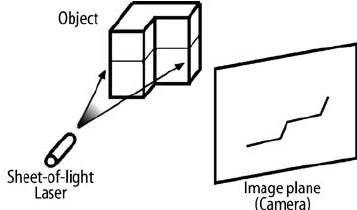
\includegraphics[width=0.5\textwidth]{./images/tech/triang_model_2.png}
  \caption{Example of laser-camera triangulation system}
  \label{fig::triang_config}
\end{figure} \\
Camera and laser are fixed each other and, at the same time, they are rotated at a known angle. In Figure \ref{fig::triang_geoms} the most common system configurations are shown. Each of them has its own pros and cons. \\

\begin{figure}[!b]
  \centering
  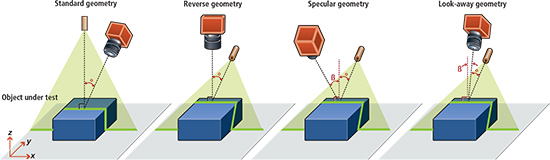
\includegraphics[width=\textwidth]{./images/tech/tech_geometry.jpg}
  \caption{Typical laser-camera configurations}
  \label{fig::triang_geoms}
\end{figure}

\noindent
In the \textit{standard geometry}, the laser line is projected perpendicularly to the $\left( x, y \right)$ nominal plane. This is the simplest configuration because the variation in the target height does not change the coordinate $y$ in the nominal plane. If on the one hand this simplifies system calibration and target shape analysis, resulting in a very fast and accurate system, on the other the camera views the object from a corner by changing the depth of field of the camera. The accommodation of the camera is needed, in order to keep the focus at the height of the object, moreover a test object must be calibrated for accurate measurement results from the system. \\

\noindent
If we switch the positions of projector and camera, we produce the \textit{reverse geometry}. In this case the system is more sensitive to the change in the height of the target, because the laser inclination causes a large shift in the position of the laser line. However these shifts change the value of the $y$ coordinate in the nominal plane, causing a more complex analysis.\\

\noindent
In \textit{specular geometry} configurations, both the projector and camera are placed at non-normal angles compared to the target surface. The placement allows a greater height resolution than the previous configurations, but the camera could see laser specular reflections. This causes noisy effect when acquiring images, such as saturation or blooming. As it happened in reverse geometry, laser inclination caused changes in $y$ coordinates when varying the height of the object. \\

\noindent
The \textit{look-away geometry} was introduced to reduce the laser specular reflections, by placing the projector and the camera at the same side of the target. However, this geometry also reduces height resolution because the camera point of view is very similar to that of the projector. \\

The \textit{standard geometry} is the most used in general purpose systems, thanks to its simplicity of implementation, calibration and use. The \textit{reverse geometry} is typically used in high resolution measurement systems, because of its performances. \textit{Specular geometry} is used, instead, when the accuracy of the system is crucial for the application of interest (such as \acs{WPMS}s), but it can be used only when the surface of the target is dark, highly textured or anyway it is a Lambert's surface. Finally, the \textit{look-away geometry} is suggested any time the target has highly reflective surfaces, such as glass or lucid metals. \\

A common issue of all these configurations is the presence of occlusions. An occlusion occurs when a non-planar target prevents the camera from seeing the laser beam. In Figures \ref{fig:occlusions} the occlusion can be seen from the point of view of the laser (Figure \ref{fig:occlusions_laser}) or from point of view of the camera (Figure \ref{fig:occlusions_camera}). This situation prevents from reconstructing the object properly, so it is often necessary to add one or more cameras or laser-camera pair to have a complete view around the object. In railway wheel analysis occlusions are a common situation to consider.
\begin{figure}[h!]
  \centering
  \begin{minipage}[c]{.50\textwidth}
  	\centering
    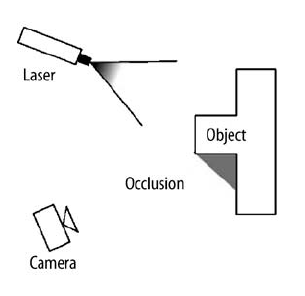
\includegraphics[width=.6\textwidth]{./images/tech/occlusion1.png}
    \subcaption{Laser occlusion}
    \label{fig:occlusions_laser}
  \end{minipage}%
  \begin{minipage}[c]{.50\textwidth}
  	\centering
    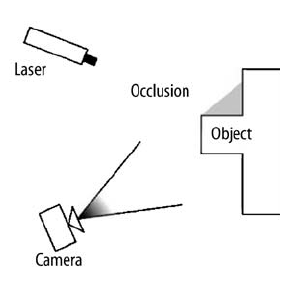
\includegraphics[width=.6\textwidth]{./images/tech/occlusion2.png}
    \subcaption{Camera occlusion}
    \label{fig:occlusions_camera}
  \end{minipage}
  \caption{Examples of different types of occlusions}
  \label{fig:occlusions}
\end{figure}

Another issue due by laser and camera relative positions, is the resolution of the camera. In 2D computer vision, the camera resolution is given by the pixel, according with the relation $resolution = \frac{Field \: of \: view}{sensor \: size}$. This is true only if the entire scene is focusable. In \acs{SOL} systems the angle between camera and laser plane prevents the focus of the entire field of view, that depends on the distance from the lens. We can distinguish three different resolutions described below. Typically, this variance in camera resolution is called \textit{trapezoidal camera resolution}. \\

\noindent
The \textit{depth resolution} is the minimum variation in the target depth appreciable by the camera. It strongly depends on the target distance from the lens and, in particular, on the angle between the projector and the camera. The greater the angle is, the greater is the variation observed in the image plane, caused by the same variation in the 3D space (in metric units). Furthermore it depends also on laser stripe thickness. Many sub-pixel approximation algorithms was developed to reduce the weight of this last factor, and some of this algorithms will be discussed later. \\

\noindent
The \textit{resolution along the laser line} is the ratio between the length of the laser line observed in the camera and the corresponding length in millimeters. As the depth resolution and because of the perspective distortion, this last resolution depends by the object distance from the camera, and it is greater close to the lens. \\

\noindent
The last is the \textit{step between consecutive frames}.
%The last is the \textit{resolution on the motion direction}.
It is present in systems that take many frames of the same object in different positions, using the same laser-camera pair. This ``resolution'' is related to the camera frame-rate and the system motion speed. \\

\noindent
The differences between them will be clearer in the Chapter \ref{ch::model}, where a complete geometric laser-camera triangulation systems model will be presented. However, we can get an idea of these differences by looking at the Figure \ref{fig:tech:resolutions}: the \textit{depth of field} is defined by the extent of the details of the focus areas. \textit{Resolution along the laser line} is given by the details appreciable by the laser itself. Finally, the tape speed and the number of captured images of the same object, define the \textit{capture step}.
  \begin{figure}[t!]
    \centering
    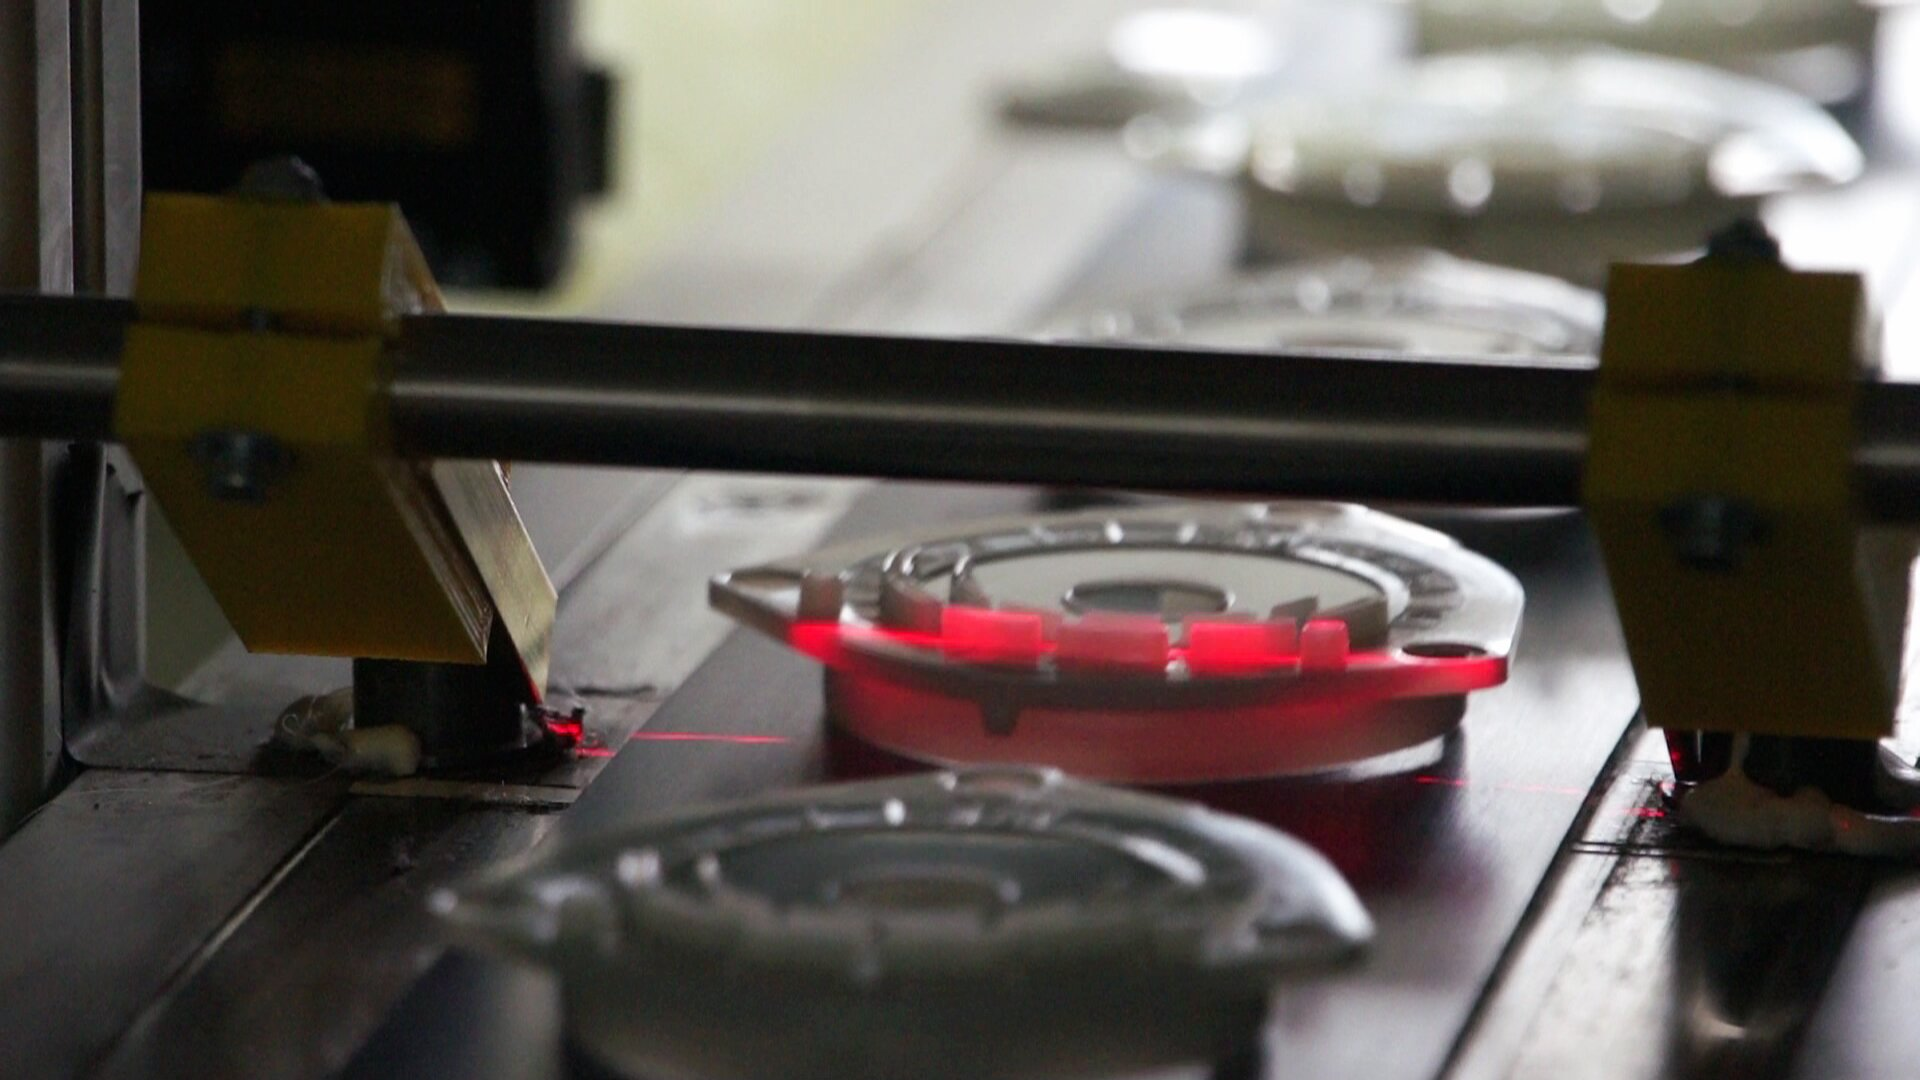
\includegraphics[width=0.8\textwidth]{./images/tech/resolutions.JPG}
    \caption{Representation of the different resolutions of a laser triangular system (property of \url{www.stemmer-imaging.co.uk}).}
    \label{fig:tech:resolutions}
  \end{figure}


% Siti di riferimento:
% http://www.vision-systems.com/articles/print/volume-20/issue-6/features/understanding-laser-based-3d-triangulation-methods.html
% http://www.aqsense.com/docs/docu_3dexpress/limits3D.html
% http://www.aqsense.com/docs/theory3D.pdf
% http://pages.stemmer-imaging.de/techforum-download/pdf/Aqsense_Understanding-and-solving-challenges-in-3D-laser-triangulation-systems_EN.pdf
% http://www.imaginasrl.it/scanner-laser.html


% Pinhole camera
  \section{Pinhole camera}
\label{sec:pinhole_camera}
Pinhole camera is the simplest camera model, where light passes through a tiny hole (from which the name \textit{pinhole camera}) of a box: an inverted image of the scene is projected on the opposite side of the box itself. This effect, known as \textit{camera obscura effect}, was studied since 500 BC (the first writings are back to the chinese Mozi) and it is the underlying principle of the $19^{th}$ century cameras. An example of the geometry of this camera is shown in Figure \ref{fig::pinhole}: as it can be seen, for each 3D point there is only one ray of light that passes through the pinhole. This is an ideal condition which allows to neglect distortions, such as blurring. Furthermore it is free of lenses, a condition that accords you to neglect distortions such as vignetting or radial and tangential distortions.
\begin{figure}[t!]
  \centering
  \begin{minipage}[c]{.48\textwidth}
  	\centering
    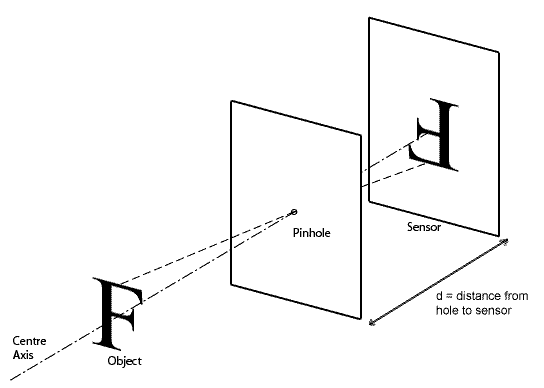
\includegraphics[width=\textwidth]{./images/tech/pinhole.png}
    \caption{The geometry of a \\ pinhole camera}
    \label{fig::pinhole}
  \end{minipage}
  \hfill
  \begin{minipage}[c]{.48\textwidth}
  	\centering
    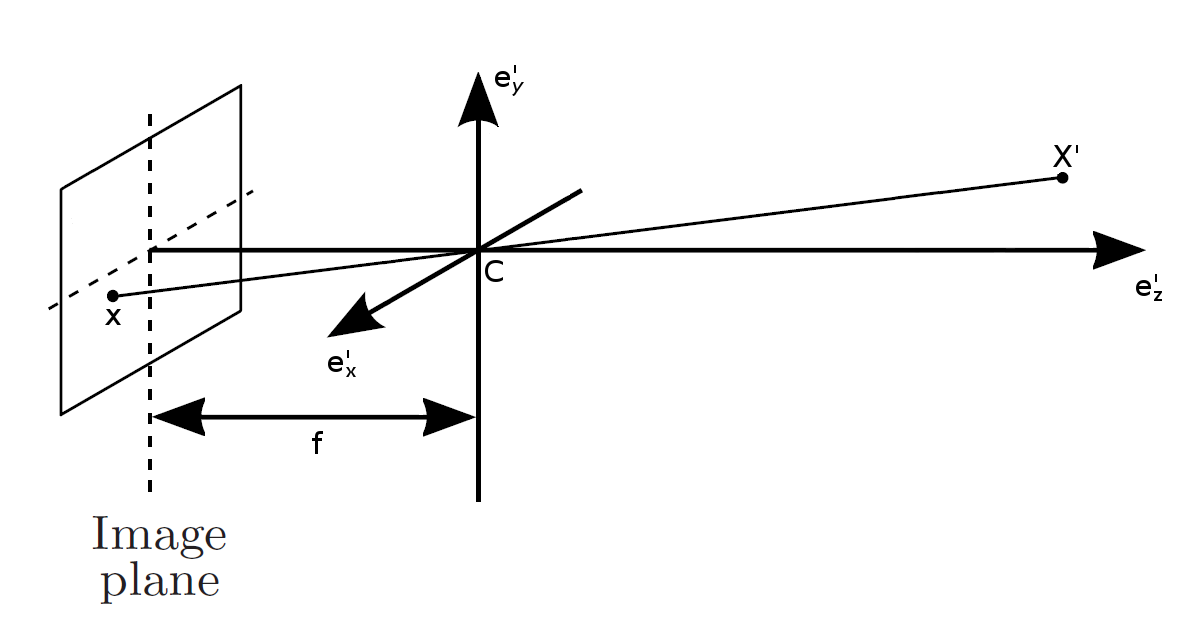
\includegraphics[width=\textwidth]{./images/tech/image_plane.png}
    \caption{Mathematical model}
    \label{fig:math_model}
  \end{minipage}
  %\caption{Examples of different types of occlusions}
  %\label{fig:occlusions}
\end{figure}

Thanks to these simplifications, the mathematical model that describes the relations between the 3D world points and their projections in the image, is very simple. Let's look at the Figure \ref{fig:math_model}. 
% Let us define the \textit{camera coordinate system} $\left(e_x', e_y', e_z' \right)$: the origin $c = \left(0,0,0 \right)$ will represent the so called camera center (i.e. the pinhole).
% We form the line between $X = \left( X_1^w, X_2^w, X_3^w \right)$ and $c$ and intersect it with the plane $z = k$ called \textit{image plane}, to generate a projection $x = (x_1, x_2, k)$ of a scene point $X$. We will refer to $e_Z$ as the \textit{viewing direction}.
% Note that if $k > 0$, the image plane is placed in front of the camera center and the image will not appear upside down. In this case we talk about \textit{virtual image}, but in real models we put $k < 0$. \\
% Since $Xc$ is a direction vector of the viewing ray we can parametrize it by the expression
%  \begin{equation*}
%    c + s(X - c) = sX \qquad s \in \mathds{R}
%  \end{equation*}
% where $sX_3^w = k$ (intersection with the plane $z = k$). Note that this model does not take into account the scene projection from the image plane to the sensor plane. \\
Let $\left(e_x', e_y', e_z' \right)$ be the \textit{camera coordinate system}, centered in $C = \left(0,0,0 \right)$, and let $C$ be the camera center (i.e. the pinhole). Then, let us define the \textit{image plane} as the 2D plane in the world in which the sensor lies. The point 2D $x = (x_1, x_2)$ in the image plane, is related to the 3D world point $X' = (X'_1, X'_2, X'_3)$ through a linear pathway for point $C$. We can parametrize this transformation with the expression:
  \begin{equation}
    \begin{pmatrix} x_1 \\ x_2 \end{pmatrix} = - \frac{f}{X'_3} \begin{pmatrix} X'_1 \\ X'_2 \end{pmatrix}
    \label{eq:image-plane}
  \end{equation}
where $f$ is the \textit{focal length} (the distance from the pinhole to which the rays are focused) of the ideal camera. This is a very simple model, but a point in the image plane does not correspond to a unique point in the world as there are three unknowns on the right hand side. Thanks to the collinearity condition from the points $X'$, $x$ and $C$, the \acs{DLT} (Direct Linear Transformation, an algorithm used to determine a set of variables from a set of similarity relations) is used: it is simple to solve this intersection and to determine this last projection. \\

However, this case is unrealistically simple, because the object and image plane are parallel. In real applications, the point $X$ can lie on a plane that have an arbitrary position and rotation, with respect to the image plane. Let us put this new plane into a \textit{global coordinate reference system} $\left( e_x, e_y, e_z \right)$; all points in the 3D world and all the camera movements will be related to this system.
% In Figure \ref{fig:math_model} we can see how point $X$ is projected in the image plane, but a questions arise: how we can locate $X$ in the world and where image plane is located respecting to the world? To answer to these questions we have to introduce a new \textit{global coordinate reference system} $\left( e_x, e_y, e_z \right)$; all points in the 3D world and all the camera movements will be related to this system.
In this way the projection of the point $X$ in the camera reference system $\left( e_x', e_y', e_z' \right)$ is a simple rotation and translation, that in \textit{homogeneous coordinates} is:
  \begin{equation}
    \label{eq:extrinsic}
    \begin{pmatrix}
      X'_1 \\ X'_2 \\ X'_3
    \end{pmatrix}
    =
    \begin{bmatrix}
      R & t
    \end{bmatrix}
    \begin{pmatrix}
      X_1 \\ X_2 \\ X_3 \\ 1
    \end{pmatrix}
    =
    H
    \begin{pmatrix}
      X_1 \\ X_2 \\ X_3 \\ 1
    \end{pmatrix}
  \end{equation}
where $R$ is a $3 \times 3$ rotation matrix and $t$ a $3 \times 1$ translation vector, and they are referred to as \textit{extrinsic parameters}, while the matrix $H$ is called \textit{homography matrix}. This is the first projection shown in Figure \ref{fig:perspective_projection}.
\begin{figure}[t!]
  \centering
  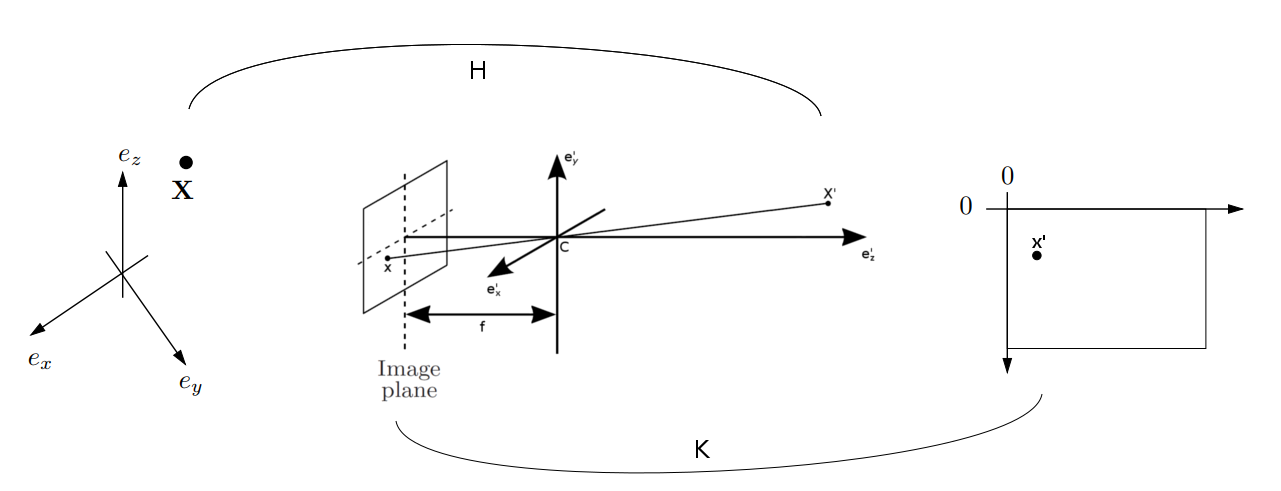
\includegraphics[width=\textwidth]{./images/tech/perspective_projection.PNG}
  \caption{Projection chain from the point $X$ in the world reference system, to $x'$ in the sensor reference system.}
  \label{fig:perspective_projection}
\end{figure} \\

The Equation \ref{eq:image-plane} shown us that the image plane is embedded in $\mathds{R}^3$, so we need to project the point $x'$ in the $\mathds{N}^2$ sensor coordinate system (in pixel unit). This is possible using a $3 \times 3$ matrix $K$ of the \textit{intrinsic parameters}
  \begin{equation*}
    \label{eq:intrinsic_matrix}
    K =
    \begin{pmatrix}
      \gamma_1	& s			& c_x \\
      0			& \gamma_2	& c_y \\
      0			& 0				& 1
    \end{pmatrix}
  \end{equation*}
where $\left( c_x, c_y \right)$ are the coordinates of the point $C$ in the sensor reference system. The pair $\left( \gamma_1, \gamma_2 \right)$ are scale factors that translate the image plane unit ($mm$) into sensor unit ($pixel$). Finally, $s$ is called skew factors, and it forces sensor rows and columns to be perpendicular. These are properties of the used camera and are related to non-ideality of camera construction. The projection (the second in Figure \ref{fig:perspective_projection}) is performed as follow:
  \begin{equation}
    \label{eq:intrinsic}
    \begin{pmatrix}
      x'_1 \\ x'_2 \\ 1
    \end{pmatrix}
    = K 
    \begin{pmatrix}
      x_1 \\ x_2 \\ 1
    \end{pmatrix}
  \end{equation} \\

The chain of all these projections, shown in Figure \ref{fig:perspective_projection}, is called \textit{perspective projection}. A common way to indicate Equations \ref{eq:extrinsic} and \ref{eq:intrinsic} in a single formula through the \textit{homogeneous coordinates} is
  \begin{equation}
    \label{eq:perspective_projection}
    \lambda
    \begin{pmatrix}
      x_1 \\ x_2 \\ 1
    \end{pmatrix}
    = KH
    \begin{pmatrix}
      X_1 \\ X_2 \\ X_3 \\ 1
    \end{pmatrix}
  \end{equation}
where the parameter $\lambda$ takes into account the projection in Equation \ref{eq:image-plane}.

%--------------------------------------------------%
\subsection{Lenses}
\label{subsec:lenses}
As mentioned above, Equation \ref{eq:perspective_projection} does not consider many non-ideality that affect the quality of images acquisitions. 

In Section \ref{sec:pinhole_camera} we introduced the fact that, ideally, only one ray per point passes through the pinhole. If on the one hand this guarantees focus, on the other the impression of the scene in the sensor requires too much time. The increasing of the size of the pinhole allows the passage of light, reducing sensor exposure time. However, in this case the projection of the point on the sensor is the result of the mixing of many light rays, condition that reduces the image sharpness until becomes a continuous smear. Lenses are used to solve this problem.

The role of the lenses is the same as the pinhole: in fact, it allows the passage of light. Their advantage compared to the pinhole is the ability to converge many light rays on a specific point, allowing much more light, and reducing film exposure times. Lens models can be quite complex, so a common practice is considered: the \textit{thin lens approximation}. A thin lens is a lens with a negligible thickness compared to the radii of curvature of its surface. In this way Equation \ref{eq:perspective_projection} remains the same. Despite this, the use of lenses introduces some other issues. \\

The amount of light that impresses the sensors is proportional to the lens diameter. The bigger the diameter is, the more light enters in the camera, but we have to consider also the \textit{magnification}. Magnification is the process of enlarging (factor greater than one) or decreasing (factor less than one, this situation is also called ``minification'') appearance of something. In this case magnification refers to the ability to see more details of the world in a single image. That said, the brightness of the image depends inversely on magnification. A simple way to indicate \textit{aperture} of a lens (the opening through which light travels), is using the \textit{f-number} $K$, defined as
  \begin{equation}
    K = \frac{f}{d}
    \label{eq:fnumber}
  \end{equation}
where $f$ is the lens focal length and $d$ the aperture diameter. As we can see in Equation \ref{eq:fnumber}, $K$ decreasing at increasing of $d$. Thanks to $K$, it is possible to compare lenses, considering image luminosity, focal length and magnification. Note that this is a simple rule with no effects on the Equation \ref{eq:perspective_projection}. \\
  
Another problem is the focus of the lens. While a pinhole camera is permanently on-focus (ideal condition), this is not always valid for a lens. In reality a lens is on focus only at a specific distance: this means that only the point at that distance will be perfectly sharp. All the other points that are out-of-focus are projected on film as circles, called \textit{circles of confusion}. The blur spot shape is due by the aperture shape (that typical is a circle from which the name) and its size increases with the distance from the focus plane. Differently from chemical film, digital sensor are made as a matrix of photosensitive elements (pixels) that convert light in electrical signals; this means that sensors resolution is not infinite. If the circle of confusion is smaller than pixels sizes, we can consider that point on focus. The space range, around the focus plane in which the scene looks reasonably sharp, is called \textit{depth of field} (\acs{DOF}). An example of these effects, common in literature, is shown in Figure \ref{fig:dof}.
%  \begin{wrapfigure}{L}{0.5\textwidth}
%    \centering
%    \includegraphics[width=0.5\textwidth]{./images/dof_txt.jpg}
%    \caption{Example of a very shallow \acs{DOF}.}
%    \label{fig:dof}
%  \end{wrapfigure} \\
  \begin{figure}[t!]
    \centering
    \begin{minipage}[c]{.48\textwidth}
      \centering
 \includegraphics[width=\textwidth]{./images/tech/dof_txt.jpg}
      \caption{Example of a very shallow \acs{DOF}.}
      \label{fig:dof}
    \end{minipage}
    \hfill
    \begin{minipage}[c]{.48\textwidth}
      \centering
 
\includegraphics[width=0.74\textwidth]{./images/tech/airydisk.jpg}
      \caption{Example of an \textit{airy disk}.\\ ~}
      \label{fig:airy-disk}
    \end{minipage}
  \end{figure} \\

The second big advantage of lenses against the pinhole, is the reduction of the diffraction. Diffraction is an effect generated by the interferences of light waves, when the light finds an obstacle or a hole, similar to the size of its wavelength. As the divergent rays now travel to different distances, some of them move out of phase and begin to interfere with each other, adding in some places and partially or completely canceling out in others. This effect, well known in many fields of interest, from electromagnetic to sound, in photography is known as \textit{airy disk} (by his discoverer, George Airy) and it is shown in Figure \ref{fig:airy-disk}. As for \acs{DOF}, even diffraction is negligible if it is smaller than the size of pixels. Diffraction could be present also in the \acs{DOF} of the camera, and depends only by the $f$-number, not by focal length. Lenses reduce this noise on the image, setting their aperture up appropriately. \\

Regardless of the lens model chosen (i.e. thin or thick lenses), their use introduces distortions due to the nature of the lens itself. In geometric optics, a distortion is a deviation from rectilinear projection, caused by small blemishes in the lenses and their alignment. The main optical aberration are two: \textit{radial distortion} and \textit{tangential distortion}. \\
Almost all of the deformation is radial in nature, this is the reason why distortion are more apparent from the center toward the edges of the image. This particular type of distortion is able to change the direction of straight lines, and it is evident during 3D calibration phases, when straight reference objects are seen from the camera as curve. Furthermore, it is often due to the need to expand the field of vision using a camera with short focal distance. Some example of its effects can be seen in Figure \ref{fig:teo-distorsions}. \\
Vice versa, tangential distortion is typically negligible than radial one, then it is ignored in most mathematical models.
  \begin{figure}[h!]
    \centering
 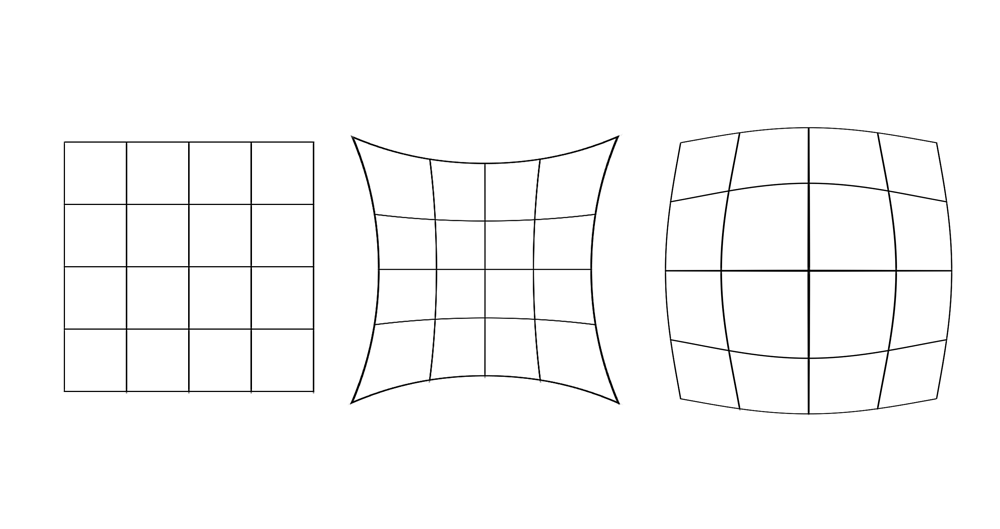
\includegraphics[width=0.9\textwidth]{./images/tech/distorsions.png}
    \caption{Example of radial distortions: on the left distortions free image is shown; in center a \textit{pincushion} aberration; on the right a \textit{barrel} aberration.}
    \label{fig:teo-distorsions}
  \end{figure}

%--------------------------------------------------%
\subsection{Scheimpflug principle}
In the previous subsection we talked about \acs{DOF} and the problem to maintain focus on the whole scene. Furthermore, we dealt with the Figure \ref{fig:dof} to show the result. Anyway, in the figure we can see that the subject lies on a plane not parallel with the sensor plane. Typical cameras and lenses are designed so that sensor plane, lens plane and subject plane are parallel to each other. This makes the focus of the camera very simple but, as said in Subsection \ref{subsec:lenses} talking about the rectilinear projection, the effective focal length depends by the position of the target with respect to the sensor itself. \\

Since the early $20^{th}$ century, the study of rotating the lens with respect to the sensor, and its effects on image acquisition, has been a widespread practice. In $1901$, Carpenter (one of the fathers of cinema) patented the first prototype of the so called ``view camera'' \cite{pat:carpentier}. From these studies, the Captain T. Scheimpflug patented \cite{pat:scheimpflug} in 1904. With his patent, Scheimpflug was the first to formulate the mathematical problem. The \textit{Scheimpflug principle} is a geometric rule that describes the relations between the sensor plane, then lens plane and the plane of focus when the lens plane is not parallel to the image plane. To achieve this situation, some cameras, such as view cameras, allow to tilt either the lens and the film, relative to the other. \\
  \begin{figure}[b!]
    \centering
    \begin{minipage}[c]{0.49\textwidth}
      \centering
      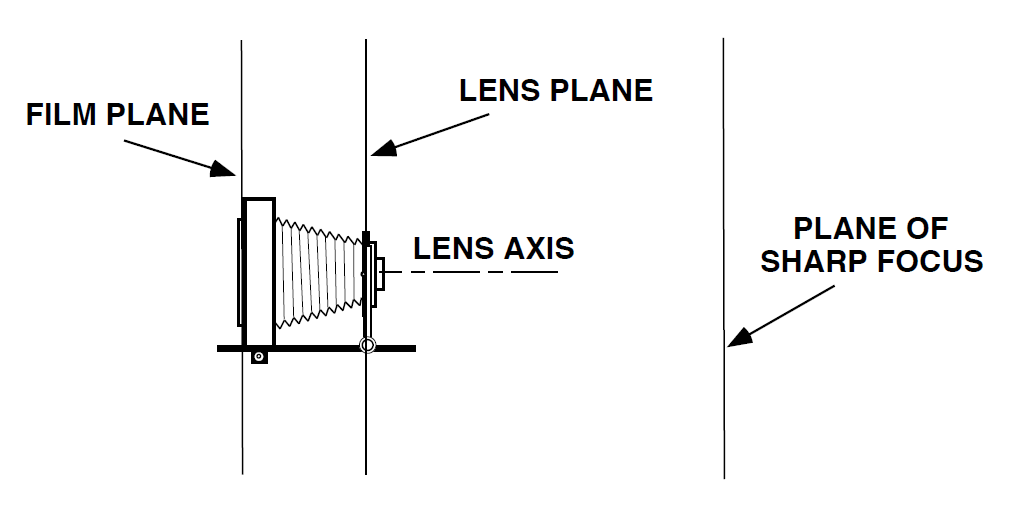
\includegraphics[width=\textwidth]{./images/tech/sch_par.png}
    \end{minipage}
    \hfill\
    \begin{minipage}[c]{0.49\textwidth}
      \centering
      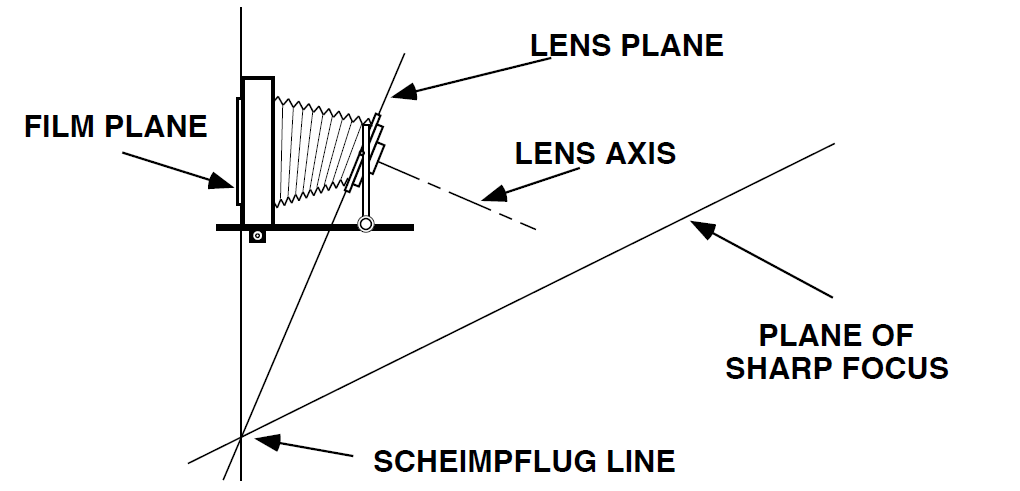
\includegraphics[width=\textwidth]{./images/tech/sch_tilt.png}
    \end{minipage}
    \caption{(On the left) For standard cameras, the sensor, lens and focus planes are parallel to one another. (On the right) For a view camera, tilting lens causes the plane of sharp focus to tilt as well.}
    \label{fig:scheimpflug}
  \end{figure}

This principle asserts that when the lens is tilted, lens plane, image plane and the plane of focus all intersects in a line, called \textit{Scheimpflug line}, as illustrated in Figure \ref{fig:scheimpflug}. In this way, a subject that is not parallel to the sensor can be completely in focus. Nevertheless, this first relation does not give any information about how to tilt the lens to achieve the intended position for the plane of focus. This information arises from the laws of optics, thanks to the \textit{hinge rule}, similar to Scheimpflug one. The required amount of lens tilt is given by the expression:
  \begin{equation*}
    \alpha = \arcsin \left( \frac{f}{J} \right)
  \end{equation*}
where $f$ is the focal length of the lens, and $J$ is the distance from the lens and the \textit{hinge line}. The hinge line is the intersection between a plane parallel with the sensor and passing through the lens one, and the plane of focus. \\
From this principle we can also determine the \acs{DOF} of the camera. It can be demonstrated that the limits of the \acs{DOF} are also planes, that passes through the hinge line, and symmetrical compared to the plane of focus. To be precise, these planes lies at a distance $J$ from the plane of focus, distance measured at the \textit{hyperfocal distance} $H$ from the hinge line \cite{book:ftvc}. The scenario is illustrated in Figure \ref{fig:sch_dof}.
  \begin{figure}[h!]
    \centering
    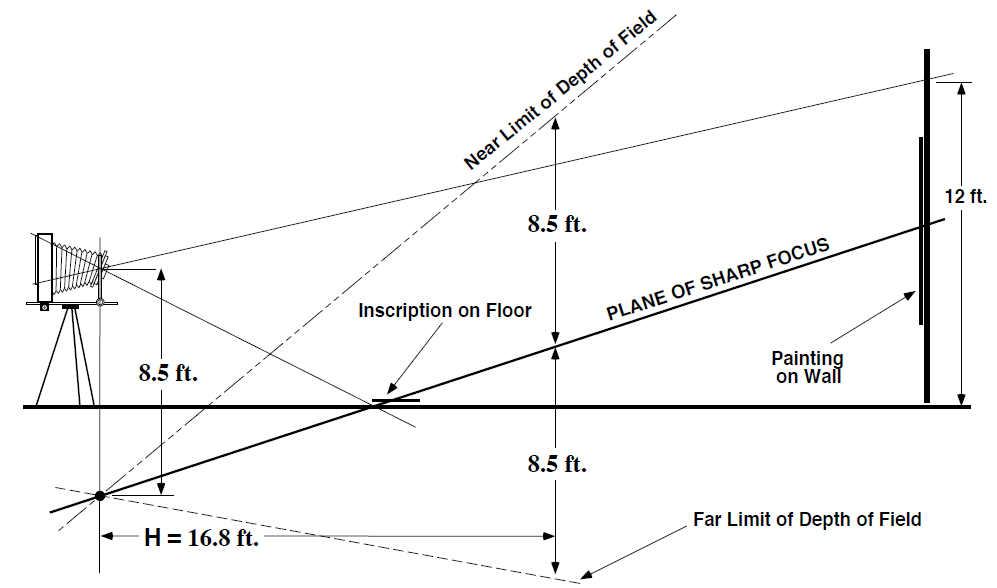
\includegraphics[width=0.8\textwidth]{./images/tech/sch_dof.png}
    \caption{Depth of field in view cameras, with tilted lenses.}
    \label{fig:sch_dof}
  \end{figure}

%--------------------------------------------------%
\subsection{Overview on digital cameras}
\label{subsec:overview-cameras}
To complete the introduction on digital camera we think that it could be useful to linger over some practical aspects, in particular about what concerns manufacturing of the sensor and image acquisitions. \\

In Subsection \ref{subsec:lenses} we introduced the quantization effect due by pixels. If it relaxes the problem of the lens focus, on the other hand it introduces noise in light to image conversion. We briefly analyse the two most popular sensor types on the market: \acs{CMOS} and \acs{CCD} (Charge-Coupled Device).

In \acs{CMOS} sensors, each element has its own signal amplifier: this allows to improve the camera frame rate and to isolate regions of interests via hardware. On the contrary, pixels haven't the same sizes neither the same doping, which reduces the quality of the sensor itself. The latest CMOS sensors on the market are good enough to be used in computer vision, achieving excellent results.

\acs{CCD} are high-scale integration sensors that use only one signal amplifier, ensuring the same amplification constant for each element. However, this requires that sensor rows are converted one by one, by lowering the camera frame rate. Furthermore these sensors give a very small, but non-zero response to a zero input and they saturate for very bright stimuli. In spite of that, they are much less noisy than the CMOS.

These differences are very delicate, specially considering the fields of application of the camera. For example, in laser triangulation systems, the acquired images are dark to highlight the laser light. In situation like this, when the brightness of the image is very low\footnote{In this case we consider source of light with brightness near to the base noise level of the sensor.}, signals amplification offsets are meaningful. The mono-pixel amplifiers in \acs{CMOS} are more noisy and generate less uniform values than \acs{CCD}, resulting in a more homogeneous output. This source of noise is known as \textit{thermal noise}. High quality systems provide different solutions to reduce this effect as much as possible. In Figure \ref{fig:thermal-noise} an example of the noise is shown.
  \begin{figure}[h!]
    \centering
    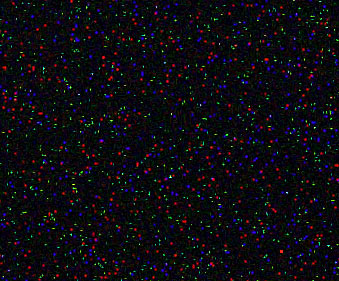
\includegraphics[width=0.5\textwidth]{./images/tech/dark-example.jpg}
    \caption{Example of uncontrolled dark noise in astronomical photography.}
    \label{fig:thermal-noise}
  \end{figure} \\

Another problem due to sensor quantization, is colours acquisition. Each pixel is able to acquire only light signals, resulting in grey scale acquisitions. For this reason sensors needed filters to encode colours. The most widespread is \textit{Bayer's color filter array} (Bayer's \acs{CFA}). A \acs{CFA} is an array in which passband filters are placed, according to a known pattern. In this way each pixel is able to encode only a specific colour. Many algorithms are used to reconstruct the scene; they interpolate signals collected by near pixels and extract the correct colour for each pixel. To perform measures, this is a waste of pixels: the presence of the filter reduces the sensor surface useful to collect world details. For these reasons, grey scale cameras are often used.


% Active light sources
  \section{Active light sources}
% According to Scott Palmer in his book Light (2013), passive and active light were at the core of Adolphe Appia's creative vision. 'The passive or diffused light refers to the general light of the stage area usually from footlights and border lights, which were common to existing stage practices at the end of the nineteenth century and were principally concerned with the widespread illumination of the stage space. In contrast, active light refers to intense, focused light that crucially allows distinct shadows to be created.
In 3D machine vision, there are many sources of light, used by the cameras to collect the information of interest. We can group these sources into two sets: \textit{passive} and \textit{active} sources. The first set refers to reflected light (typically used in photography), that is ``the general light of the stage area [\ldots] and were principally concerned with the widespread illumination of the stage space'' \cite{palmer2013light}. The second set refers to all intense and focused lights that create distinct shadows on the scene.
% Per quanto riguarda i sistemi basati su triangolazione ...
As far as triangulation-based systems are concerned, we are only interested in active sources, in particular in \acs{LASER}. \\

A \acs{LASER} is a device that emits a coherent light beam, and originally its name was the acronym of \textit{Light Amplification by Stimulated Emission of Radiation}. It comes from the physical processes used to generate the light beam: when an incoming photon (at a specific frequency) interacts with an excited electron, the electron changes its energy level. The energy liberated when it returns to its initial state, generates a new photon, completely identical to the first one. Now, the four main parts that compose this device are:
  \begin{itemize}
    \item The \textit{active medium} is the source of optical gain.
    \item The \textit{pumping system}, that provides the energy needed to excite photons.
    \item The \textit{cavity resonator}, where the photons are reflected back and forth between the cavity's walls.
    \item The \textit{collimator}.
  \end{itemize}
As far as the last point is concerned, it is not a fundamental element from the point of view of the \acs{LASER} itself, but for its use in measuring systems. In fact, as we will describe later, the emitted light has the shape of a spot. To spread it along a line, a collimator is needed. A collimator is a particular curved lens, putted in front of the \acs{LASER}, that filters the stream of rays so that only those travelling parallel to a specified direction are allowed through. In this way, it is possible to spread the light power on a plane and to obtain a \acs{LASER} line on the target.\\

The main properties of the \acs{LASER}s are their temporal and spatial coherences. The spatial coherence allows the \acs{LASER} to be collimated: this means that the rays of light are all parallel to each other, generating the typical shape of a spot. For this reason, in \acs{SOL} systems it is common to put a \textit{collimator} in front of the \acs{LASER}, in this way the energy of the collimated spot is spread to a plane, that is a line when it hits a target object. \\
Temporal coherence, instead, allows the \acs{LASER} to emit light with a very narrow spectrum, i.e. they are monochromatic. \\
Thanks to their coherencies, the \acs{LASER}s can focus a great amount of energy on a very small areas, allowing their use in a wide range of applications. Depending on the field of application, we can find \acs{LASER}s with different wavelengths, both in visible and invisible spectrum. \\

  \begin{table}[b!]
  \begin{tabular}{|c|p{12cm}|}
  \hline
  \multicolumn{1}{|c|}{\textbf{Class}} & \multicolumn{1}{c|}{\textbf{Description}} \\
  \hline
  
  1  &
  \acs{LASER}s that belong to this class are always safe for the human health. Generally the emitted power is $P < 0.04 mW$, but in this class there are also that \acs{LASER}s that prevents the direct interaction of the operator (such as laser printers). No protection is required. \\
  \hline
  
  1M &
  This class differs from the previous one because these are dangerous \acs{LASER}s, if used in pair with optical instruments. Typically, their works in the range $\left[302.5, 4000\right] nm$. \\
  \hline
  
  2  &
  These are low-power \acs{LASER}s $\left( P < 1 mW\right)$ that emit in the visible spectrum $\left( 400, 700 \right) nm$. This type of \acs{LASER}s are not inherently safe, but the eyelid is enough to protect eyes from incidental reflections. It is important not to look them directly. \\
  \hline
  
  2M &
  Like the class 1M, \acs{LASER}s belonging to this class refer to class 2 too, but are dangerous if used in pair with optical instruments. \\
  \hline
  
  3R &
  This is the first class of \acs{LASER}s that are really dangerous for humans. Here we find \acs{LASER}s that emit in the visible spectrum $\left(302.5, 106\right) nm$. They can injure eyes even if viewed indirectly. \\
  \hline
  
  3B &
  Like the class 3R, we can find \acs{LASER}s dangerous both for eyes and skin. They emit beams with power under $500 mW$. \\
  \hline
  
  4  &
  Like the class 3B, \acs{LASER}s that belong to this class are dangerous for eyes and skin, even in diffuse radiation, and they can cause fires. Another source of danger are their very high working voltage and current. We have to be very careful when we use this class. \\
  \hline
  \end{tabular}
    
  \caption{Classes of \acs{LASER}s and their regulations} 
  \label{tab:laser-classes}
\end{table}
Nevertheless, lasers coherence can be a risk factor for the health of users. Because of their differences in wavelength, emitted power and pulse frequencies, it has been necessary to rule their use, and to group them, accordingly with their properties. \acs{CEI} grouped \acs{LASER}s in five classes, accordingly with regulations \cite{cei:76-2}, in order to define the \acs{MPE} (Maximum Permissible Exposure) for each category, i.e. the maximum exposure time in which the damage for the health is negligible. These classes are described in Table \ref{tab:laser-classes}. The choice of the correct class needed in our project is very important, in particular in industrial systems. For our tests, described later, we used \acs{LASER}s belonging to classes 1 and 2. \\

% --------------------------- %
\subsection{Peak detection}
\label{subsec:peak-detection}
An important aspect of lasers is their mathematical modelling. The accuracy of triangulation-based systems, and in general of laser-based systems, is significantly determined by the detection of the laser stripe. \\

In literature there are many models that try to describe laser stripes, but the most used is the \textit{Gaussian} shape that, accordingly with \cite{saleh2013fundamentals}, we can generalize as:
  \begin{equation}
    e^{-jkz}
    \label{eq:general-gauss-model}
  \end{equation}
where $k = \frac{2\pi}{\lambda}$ is the wavenumber with wavelength $\lambda$, and $z$ is the direction of propagation of the signal. This model is quite simple, because it approximates the spot laser with the point of maximum light intensity (peak of the Gaussian). Furthermore this model is symmetrical with respect to the center of the spot, guaranteeing the shape shown in Figure \ref{fig:laser-spot-gauss}. Like camera lenses, also lasers have to be focused. Since the beam has its minimum width at $z = 0$, this will be the best focus plane. Moving in both directions, the width of the beam grows ``out of focus''. When the width of the beam is $\sqrt{2}$ the initial width, we have reached the laser \textit{depth of focus}.
  \begin{figure}[t!]
  \centering
    \begin{minipage}[c]{.48\textwidth}
      \centering
      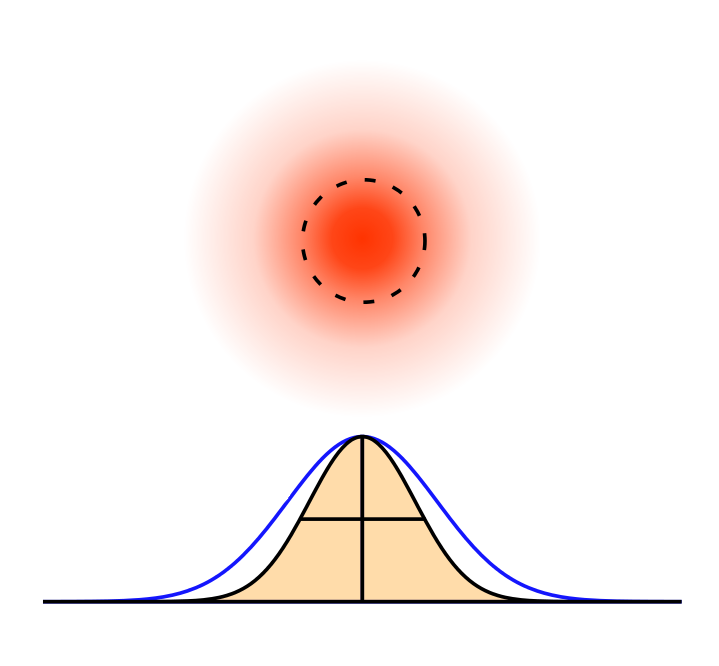
\includegraphics[width=0.8\textwidth]{./images/tech/laser-gauss.png}
      \subcaption{Gaussian model.}
      \label{fig:laser-spot-gauss}
    \end{minipage}
    \hfill
    \begin{minipage}[c]{.48\textwidth}
      \centering
      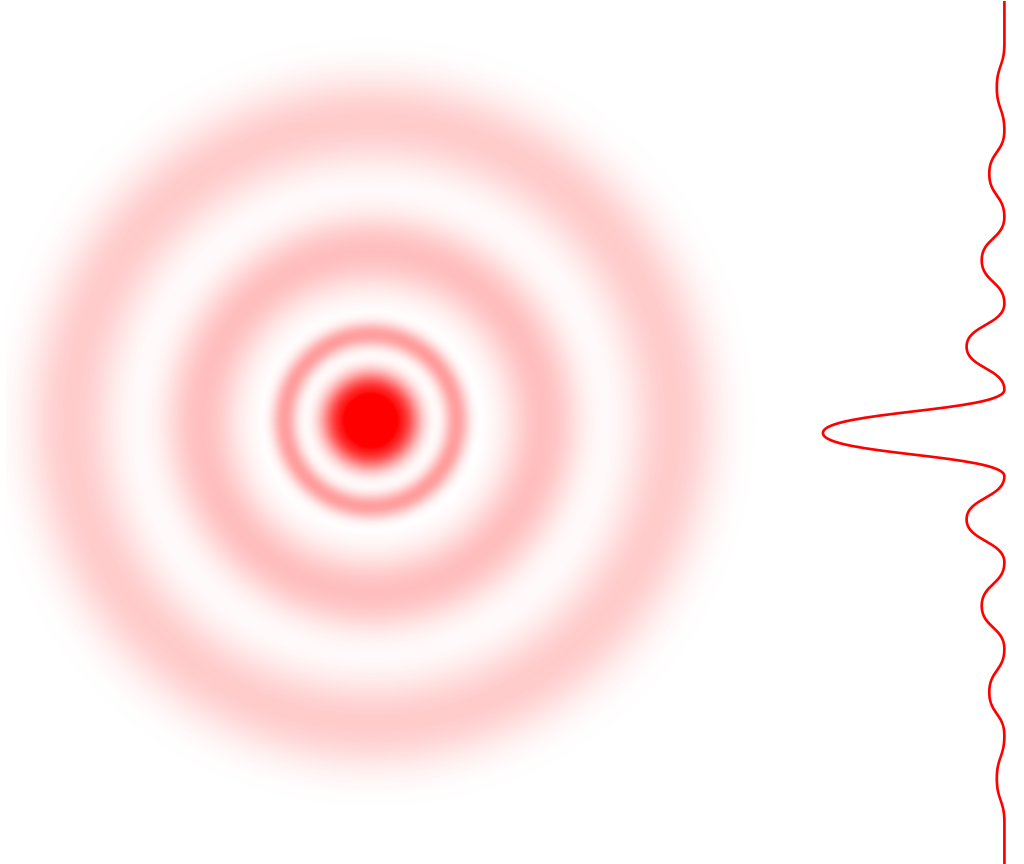
\includegraphics[angle=270, origin=c, width=0.64\textwidth]{./images/tech/laser-bessel.png}
      \subcaption{Bessel model.}
      \label{fig:laser-spot-bessel}
    \end{minipage}
    \caption{Models for lasers spots.}
    \label{fig:laser-spot-models}
  \end{figure}

Another solution, proposed in \cite{saleh2013fundamentals}, is the \textit{Bessel} laser model. As we can see in Figure \ref{fig:laser-spot-bessel}, this model is very similar to the Gaussian one: it has a global maximum and it is symmetrical with respect to its center. The interesting thing is the fact that it is diffraction free and has a bigger depth of field than the Gaussian model. \\

Before going deeper in the problem of laser extraction from an image, it is important to introduce the \textit{speckle noise}. Speckle noise is a granular noise that inherently exists in all coherent sources (lasers, radars, SAR, ...). It is generated when a coherent signal strikes a rough surface, spreading random radiation into space. Thanks to their coherence, the radiations are identical to the original signal, but some of them change their phase, interfering with each other. The interferences can be constructive or destructive, and what we see in the image plane is a dotted spot. The effects of this noise change if we vary the wavelength of the laser, the aperture of the lens and the setup of triangulation system, but the main important thing is that, accordingly with \cite{Baribeau:91},\cite{Dorsch:94} and \cite{Hausler:88}, this noise is a limit for the determination of the precise position of the spot in the image. \\

Once we have defined these models, the next step is to locate the laser position in the image. To do that, we can consider each row of the image as a Gaussian, defined by the value of the pixel belonging to that row, as shown in Figure \ref{fig:tech:laser-prof}. Thanks to shape and symmetry of the Gaussian distribution, it is common to look for the pixel of greatest light intensity, that ideally is located under the peak of the laser. Using this approach for each row of the same frame, we can obtain the results shown in Figure \ref{fig:tech:laser-example}.
%Once we have defined these models, the next step is to locate the laser position in the image. To do that, we can consider each row of the image as a Gaussian, defined by the value of the pixel belonging to that row. In Figure \ref{fig:tech:laser-prof} we shown a representation of this assumption. Thanks to shape and symmetry of the Gaussian distribution, it is common to look for the pixel of greatest light intensity, that ideally is located under the peak.
% Once we have defined these models, the next step is to locate the laser position in the image. Thanks to their shape and symmetry, it is common to look for the pixel of greatest light intensity, that ideally is located under the peak.
However, as we can see in Figure \ref{fig:gauss-discr} this is not completely correct: the discretization introduced by the physical structure of the sensor, forces the Gaussian to stay in the middle of the pixel, and in some cases (such as the one illustrated in Figure) if the peak is between two pixels, we make an error regardless of the pixel we choose. From the point of view of the accuracy of the measure, this approximations are too coarse to satisfy the typical industrial requirements. \\

  \begin{figure}[t!]
    \centering
    \begin{minipage}{\textwidth}
      \centering
      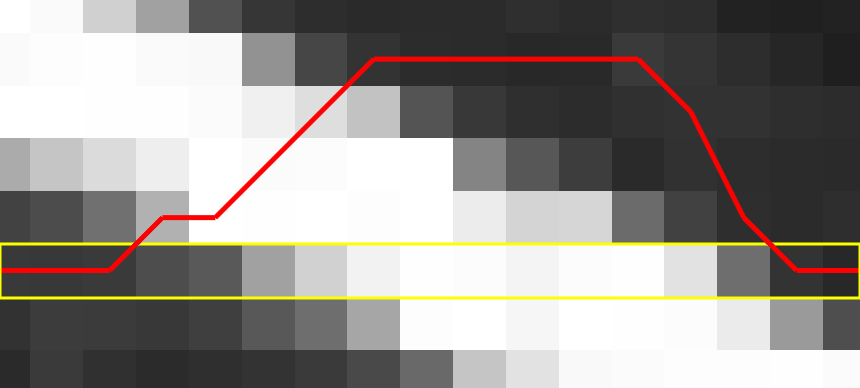
\includegraphics[width=0.8\textwidth]{./images/tech/laser_prof.png}
      \caption{Gaussian approximated distribution of the highlighted line.}
      \label{fig:tech:laser-prof}
    \end{minipage}
    \vfill
    \begin{minipage}{0.49\textwidth}
      \centering
      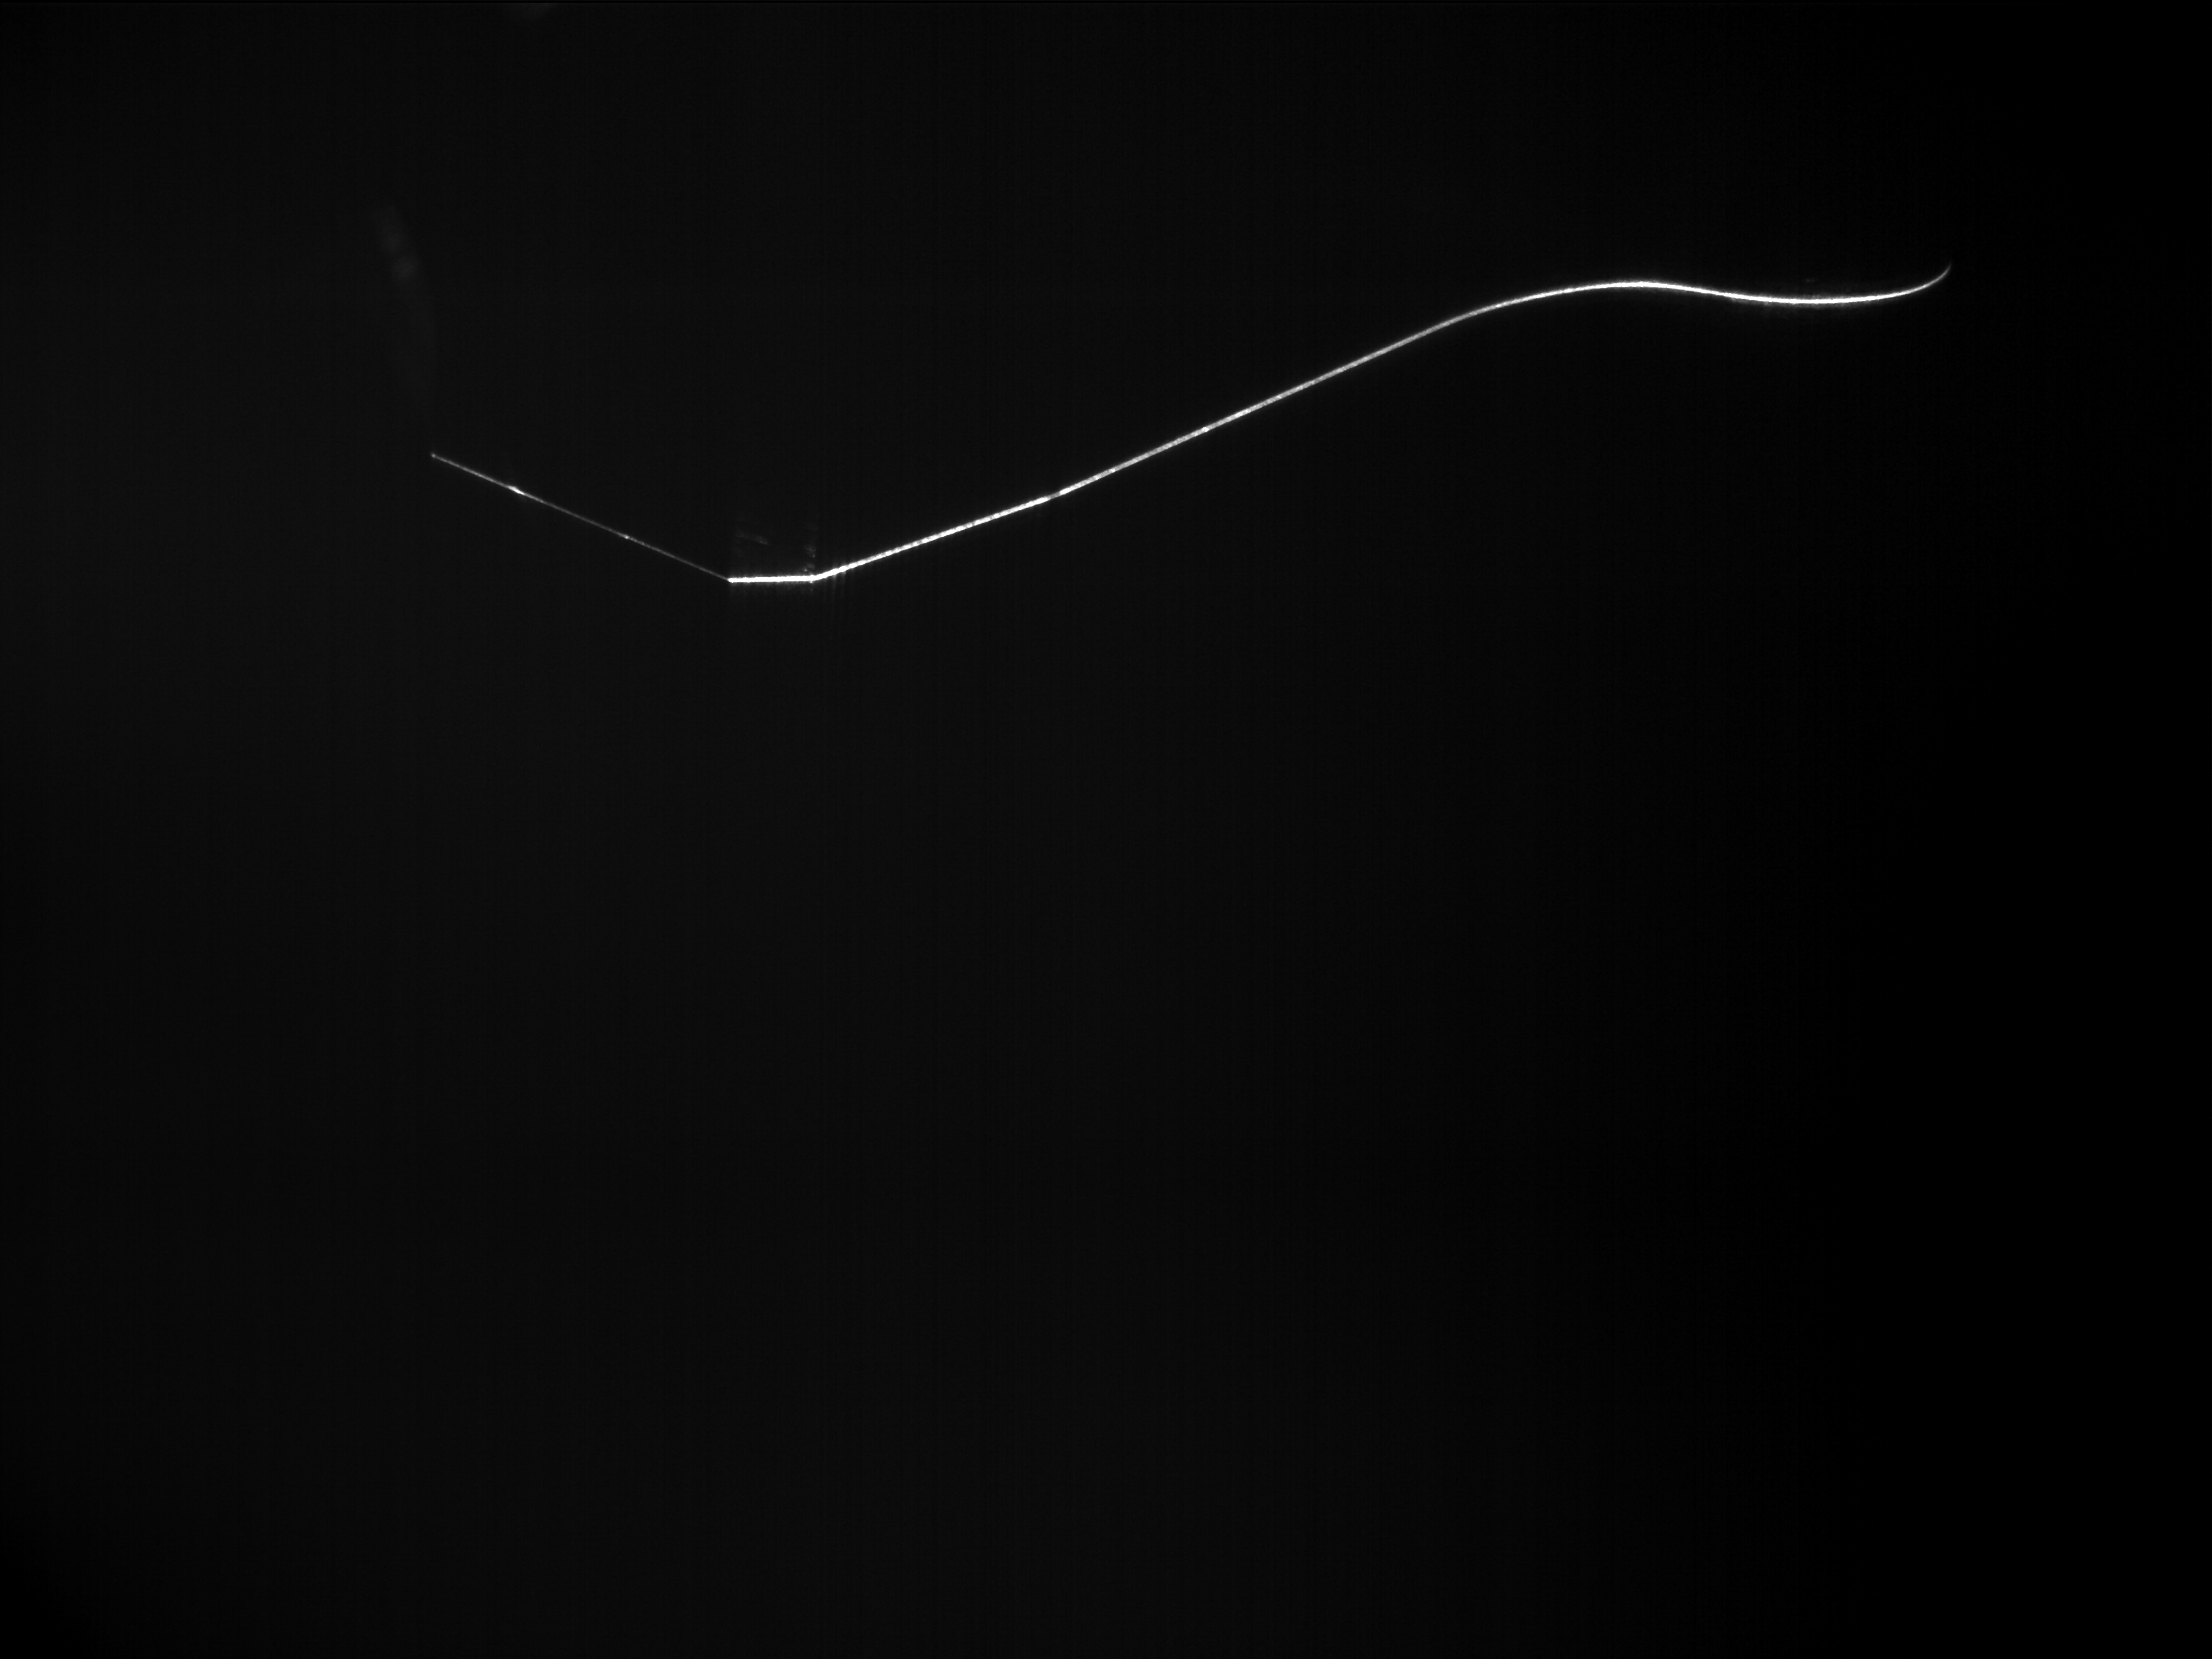
\includegraphics[width=\textwidth]{./images/tech/C0_p240_SD.png}
    \end{minipage}
    \hfill
    \begin{minipage}{0.49\textwidth}
      \centering
      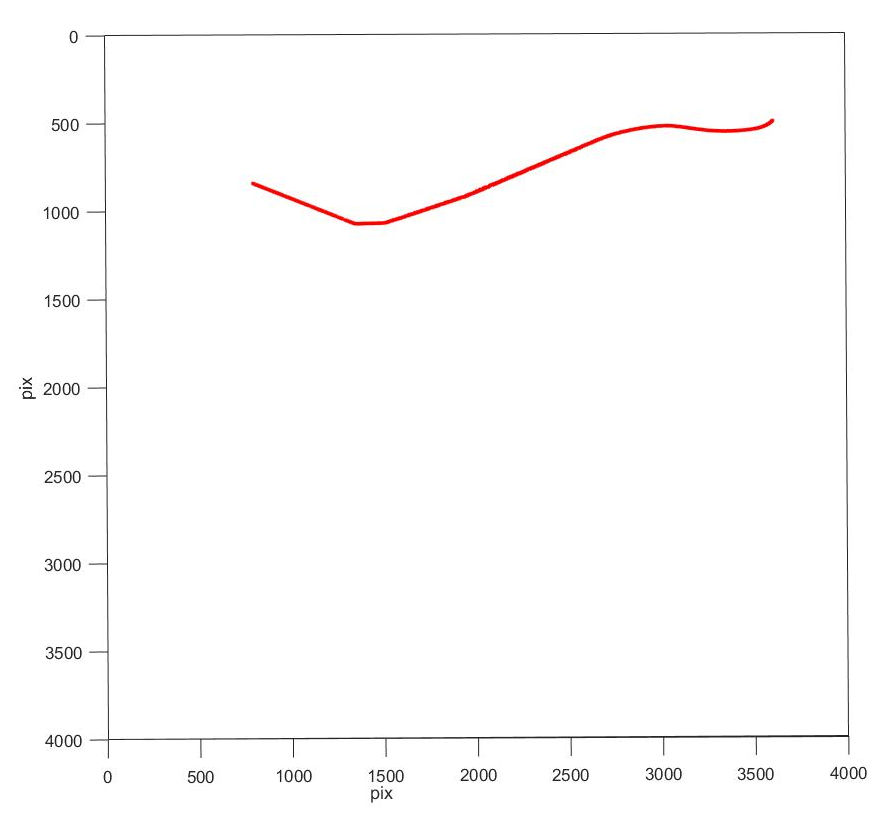
\includegraphics[width=0.9\textwidth]{./images/tech/profile_ex.jpg}
    \end{minipage}
    \caption{Example of profile extraction. On the left there is a live frame of a railway wheel, while, on the right, there is the extracted profile.}
    \label{fig:tech:laser-example}
  \end{figure}
\vfill
  \begin{figure}[t!]
    \centering
    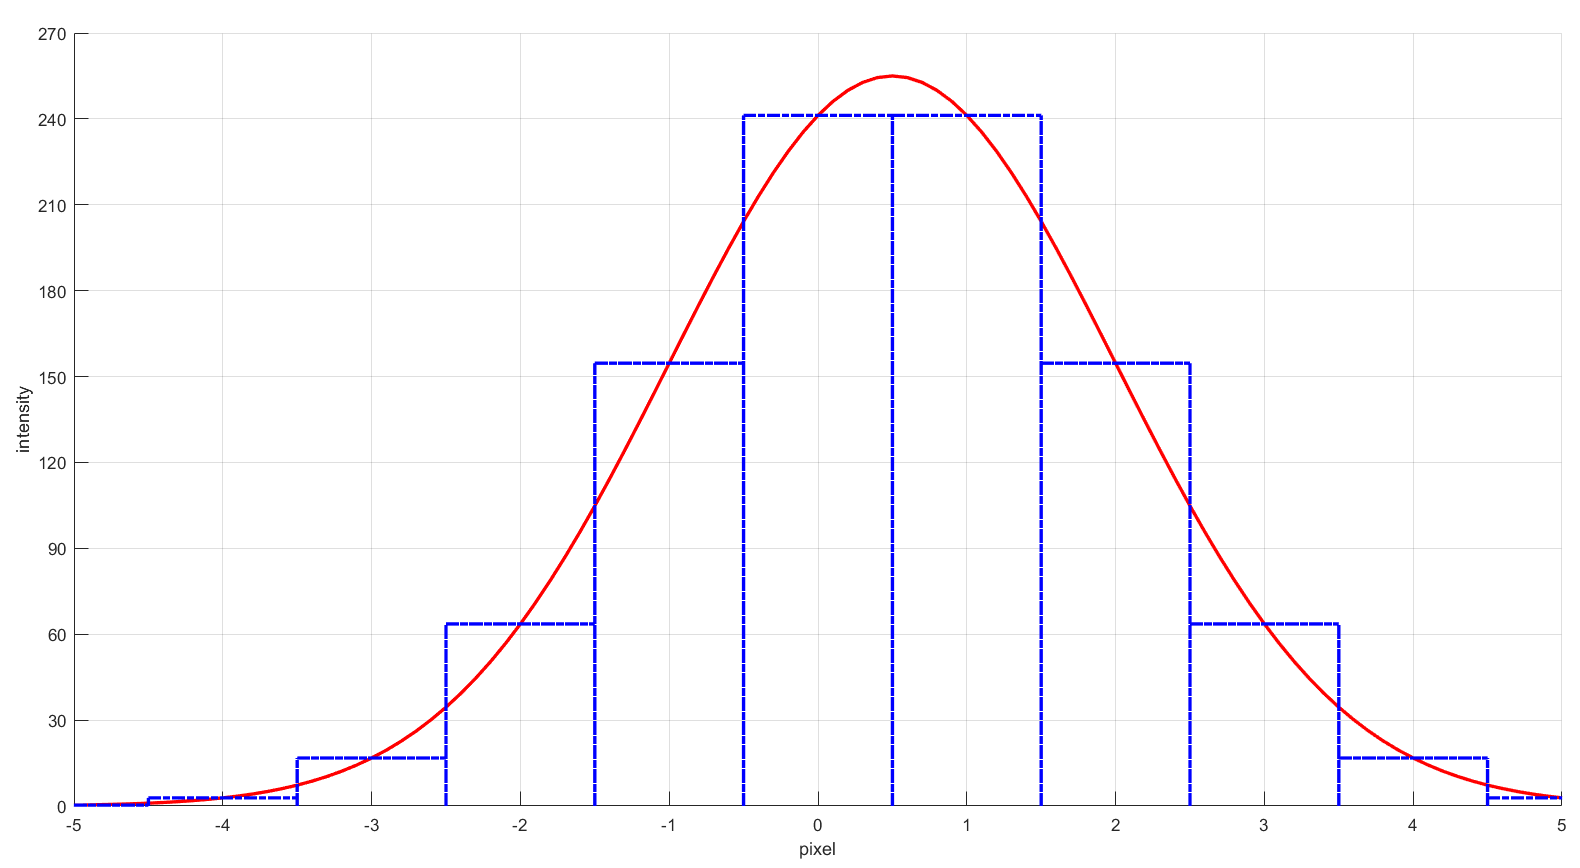
\includegraphics[width=0.79\textwidth]{./images/tech/gauss-discr.png}
    \caption{Gaussian distribution discretization because of pixels.}
    \label{fig:gauss-discr}
  \end{figure}

To try to solve these problems, in literature we can find a lot of solutions, such as in \cite{BLAIS1986145}\cite{Dorsch:94}\cite{1334612}\cite{Naidu1991}\cite{doi:10.1080/095119298130642}.
All of the proposed filters try to approximate the shape of the Gaussian model, starting from the light intensities collected by the pixels, and in this way the peak location with subpixel accuracy is improved. \\
To better understand how these filters works, we grouped them in two categories:
  \begin{itemize}
    \item the first one gathers all that filters that use mathematical relations to fit a Gaussian distribution over the pixels;
    \item the second one gathers all that filters that compute the discrete derivatives of the discrete signal, and use them to locate the global maxima.
  \end{itemize}
Given the pixel collected by the greatest amount of light intensity, all the filters described below locate the peak of the spot using only the pixels along the $y$ axis, consistently with the coordinate reference system used in Section \ref{sec:init-modelanalysis} (parallel to the direction of the laser beam).

In the following of this section, we will indicate with $y$ the coordinates of the pixel candidate to contain the peak of the spot laser, while with $b$ the light intensity collected by that pixel. Then we will indicate with $a$ and $c$ the light intensities collected by the pixels $y-1$ and $y+1$, respectively.

% --------- %
\subsubsection{Centre of Mass (\acs{COM})}
The \acs{COM} (known as \textit{Center of Gravity}, \acs{COG}) is probably the most used subpixel filter. It tries to determine the peak of a gaussian distribution implementing a sliding window mean. Given $a$, $b$ and $c$, we can write:
  \begin{equation}
    \hat{Y} = y +\frac{c - a}{a + b + c}
    \label{eq:sp-com}
  \end{equation}
In literature, it is known that this filter is very sensitive to the noise in the image, in particular it is sensitive to the thermal noise.

% --------- %
\subsubsection{Gaussian approximation}
This filter is based on the idea that the laser spot is similar enough to a Gaussian distribution: as we will see later, this condition is never satisfied because of the thermal noise of the camera. Mathematically, the peak is given by:
  \begin{equation}
    \hat{Y} = y - \frac{1}{2}\left( \frac{\ln{c} - \ln{a}}{\ln{a} - 2\ln{b} + \ln{c}} \right)
    \label{eq:sp-gauss}
  \end{equation}
As we can see, this filter uses only three pixel to determine the position of the peak.

% --------- %
\subsubsection{Linear Interpolation}
Linear interpolation filter simply assumes that a linear relation exists among the usual three points
  \begin{equation}
    \hat{Y} = \begin{cases}
      y - \frac{a - c}{2(b - a)} \qquad if \quad c > a \\
      y - \frac{a - c}{2(b - c)} \qquad otherwise \\
    \end{cases}
    \label{eq:sp-linear}
  \end{equation}

% --------- %
\subsubsection{Parabolic Estimator}
Unlike the previous filter, the parabolic estimator tries to use a continuous vision of the laser signal, so it derives from the Taylor decomposition of the light intensity near the peak.
Let $\delta \in \left[ -\frac{1}{2}, \frac{1}{2} \right]$ be the variation of the peak position with respect to the center of the pixel $y$, and let $f(y + \delta)$ the real value of the peak. Thus, we can write:
  \begin{equation}
  \delta = \frac{f'(y)}{f''(y)} = \frac{f(y+1) - f(y-1)}{2\left( f(y+1) - 2f(y) + f(y+1)\right)}
    \label{eq:sp-parabolic}
  \end{equation}

% --------- %
\subsubsection{Blais and Rioux Detectors}
This filter was originally proposed in \cite{BLAIS1986145}. The original idea was to use a linear interpolator in cascade on a finite impulse asymmetrical digital filter. The authors obtained a linear filter insensitive to laser spot amplitude and, at least theoretically, more robust with respect to the \acs{COM}. Let $f(y)$ be the same function defined for the parabolic estimator, and let $g_d(i)$ a function defined as:
  \begin{equation*}
    g_d(i) = \sum_{k=-d/2}^{-1} f(i + k) - \sum_{k=1}^{d/2} f(i + k)
  \end{equation*}
The estimation of the peak position is given by
  \begin{equation}
      \delta = \frac{g(y)}{g(y) - g(y+1)} 
    \label{eq:sp-br}
  \end{equation}
if $f(y+1) > f(y-1)$; otherwise we will write: $\delta = \frac{g(y-1)}{g(y-1) - g(y)}$.
  
% --------- %
\subsubsection{FIR filter approach}
The last filter we are interested in, is the FIR. As a FIR filter, this one tries to evaluate the discrete derivative of the Gaussian distribution, and looks for the point in which the derivative intersects the origin: that point will be the peak position. We can use the following relation to describe what said so far:
  \begin{equation}
    \hat{Y} = y_0 - \frac{I_0 \cdot \left( y_1 - y_ 0\right)}{I_1 - I_ 0}
    \label{eq:sp-fir}
  \end{equation}
where $I_i$ is the intensity of light collected by the sensor in the pixel; $(y_0, I_0)$ are the coordinate and the intensity of the last point before the origin, while $(y_1, I_1)$ are the coordinate and the intensity of the first point after the origin.

Also in this case, we assume that the error committed locating the peak position is at most half pixel. \\

\bigskip
As we can see, all the filters above are introduced using only three pixels. In real systems this could not be enough to reach a good precision in the measures, generally because of the depths of field of cameras and lasers. Moreover, laser beams can be as thick as $30$ pixels: in these cases, considering only three pixels makes the final approximation very partial, and in saturation conditions the problem is what pixels must be considered. Furthermore, as just mentioned, they are sensitive to the presence of noise in the image. In particular, the thermal noise (described in Subsection \ref{subsec:overview-cameras}) has to be removed before to exploit subpixels optimizations, for example subtracting the background noise of the camera.
Accordingly with \cite{1334612} and \cite{Naidu1991}, Filters \ref{eq:sp-gauss}, \ref{eq:sp-linear}, \ref{eq:sp-parabolic}, \ref{eq:sp-br} and \ref{eq:sp-fir} should be better than \ref{eq:sp-com}, but our analysis shown something different.


% The camera calibration problem
  \section{The camera calibration problem}
\label{sec:teo-calibration}
The \textit{geometric camera calibration} is a process that allows to determine all the parameters introduced with the Equation \ref{eq:perspective_projection}. When we calibrate a single camera, we are determining only its intrinsic parameters, instead if we calibrate a couple of cameras (or, as in this case, a laser-camera pair) we are able to locate the points in the 3D space, and we can determine the extrinsic parameters of the equation. Accordingly with what we said in Subsection \ref{subsec:lenses}, lens distortions are critic when we need to reconstruct the 3D world from an image, so they have to be considered by calibration algorithms that, generally, implement non-linear optimization methods (note that the general model for lens distortions is non-linear). Furthermore, some algorithms (such as \cite{SchCameraCalib} and \cite{hamrouni2012new}) try to consider the distortion due to the lens tilt caused by, in turn, the use of the Scheimpflug principle. \\

In literature there is a multitude of calibration algorithms, most developed for stereocamera systems. In this subsection we briefly introduced two algorithms that can be used to calibrate laser triangulation systems, proposed by Tsai \cite{TsaiTvLenses} (the pioneer of camera calibration algorithms) and Zhang \cite{Zhang-calib}. Both the algorithms are based on the pinhole projective model, described in Equation \ref{eq:perspective_projection}, and take in input a grid of points, both in image and world reference systems, and give in output the camera parameters. As we can understand, the origin of the world reference system could be arbitrary, but the system must be consistent with the world.

The choice of to use these algorithms was done by their interest in our filed of study and by the availability of data to compare. However, the use of non-linear optimizations made it difficult to estimate some parameters of interest for the next analysis.

\subsubsection{Tsai}
Roger Tsai proposed its algorithm in 1987 in order to improve the already existing algorithms, that lacked of many informations, such as lens distortions. Thus, he introduced a two-step process: in the first step he evaluated the intrinsic parameters starting from the grid took in input; in the second step he applied a non-linear optimization to correctly evaluate intrinsic parameters, with particular attention with focal length and lens distortions. As shown in his article, he developed a very accurate, fast and versatile algorithm to calibrate cameras. Furthermore, one of the advantages of this technique is the ability to calibrate using a single planar view of the reference target. \\

As we can read in the Reg Wilson's FAQ\footnote{\url{http://www.ius.cs.cmu.edu/IUS/usrp2/rgw/www/faq.txt}, no longer available now.} we have to be cautious when we set Tsai parameters. First of all, it assumes that some nominal values, such as pixel sizes, sensor size and frame grabber are correct. In this way he simplifies some passages of the algorithm. Second we have to pay attention on the choice of the world reference system: if we consider the coplanar procedure, the origin of our coordinate reference system must to be far from the center of the sensor, otherwise the algorithm could be not work. \\
Both in coplanar and non-coplanar procedure, the input grid must have at least $11$ point to calibrate correctly. Furthermore, the points have to be taken broadly across the \acs{FOV} to let the non-linear optimization work properly. \\

Note that, in order to separate the effects of $f$ and $T_z$ on the image, there needs to be perspective distortion effects in the calibration data. For useable perspective distortion, the distance between the calibration points nearest and farthest from the camera should be on the same scale as the distance between the calibration points and the camera. This applies both to coplanar and non-coplanar calibration:

For co-planar calibration the worst situation is to have the 3D points lied in a plane parallel to the camera's image plane (all points at   equal distance away). Simple geometry tells us we can't separate the effects of $f$ and $T_z$. A relative angle of $30$ degrees or more is recommended to give some effective depth to the data points.

For non-coplanar calibration the worst case is to have the 3D points lied in a volume of space that is relatively small compared to the volume's distance to the camera. From a distance the image formation process is closer to orthographic (not perspective) projection and the calibration problem becomes poorly conditioned.


\subsubsection{Zhang}
Zhang developed an hybrid process that combines self-calibration (a grid similar to that of Tsai) and traditional calibration techniques (match between the same point in different images), which enables the linear estimation of all intrinsic parameters. To do that at least three images of a well known planar pattern (or reasonably considered such) are needed, taken in different positions. The motion of the pattern should not necessarily be known. The steps needed to calibrate the system are the following, to:
  \begin{enumerate}
    \item Print a pattern and attach it to a planar surface.
    \item Take a few images of the model plane under different orientations by moving either the plane or the camera. In the scenarios we are interested in, we will move the pattern keeping fixed the camera.
    \item Detect the feature points in the images.
    \item Estimate the five intrinsic parameters and all the extrinsic parameters using the closed-form solution.
    \item Refine all parameters, including lens distortion parameters.
  \end{enumerate}
Unlike Tsai, Zhang tries to estimate the lens distortions until the fourth degree. As the author admitted in the original paper, his algorithm could degenerate if the pattern took in the different frames, lies in parallel planes.

\bigskip
Now we can understand the importance of planar calibration algorithm in laser-based triangulation systems: the laser forms a flat plane in the 3D world reference system. All points we will acquire lie on this plane. From this point of view, Tsai is preferable with respect to Zhang, because it used a single view of scene, taken on the laser plane. Note that if we use a known pattern (i.e. a checkboard), we must be sure that the pattern lies on the laser plane, otherwise the map that obtained will be incorrect.

  % \clearpage

% 3D computer vision overview
  \section{3D computer vision overview}
The laser-camera triangulation system is not the only way to perform 3D world reconstruction. The most commonly used technologies are:
\begin{itemize}
  \item \textsc{Stereo Vision} - The typical stereo vision system is a binocular system, composed by two cameras displaced horizontally, viewing the same scene at two slightly different angles. Thanks to the epipolar geometry it is possible to determine where a specific 3D world point is projected into the 2D planes of the two cameras. After determining these relations, the relative depth information can be obtained in the form of a disparity map, which encodes the differences in horizontal coordinates of corresponding image points. The values in this disparity map are inversely proportional to the scene depth at the corresponding pixel location.
  
  \item \textsc{Structured light} - Similarly to \acs{SOL} technology, structured light sensors are made by a camera and by a source of light (DLP-projector) that project know patterns, alternating bright and dark. Patterns are deformed because of the shape of the target as with \acs{SOL}, and triangulation is used for the 3D reconstruction. The main benefit of using a DLP-projector rather than a fixed light line is that the projection project the pattern over the whole scene, and mechanical translation or motion required by SOL is not required.

  \item \textsc{Time Of Flight (\acs{TOF})} - This technique is the youngest of the ones proposed. \acs{TOF} sensors estimate distances by measuring the time needed to a signal (light, electromagnetic, acoustic, ...) to reach an obstacle and come back to the sensor. One of the benefits of using this technique is the independence of the calculated distances for each pixel, allowing very high accuracy, but this type of sensors are very delicate and require a lot of handling. \acs{LIDAR} (Light Detection And Ranging) is the first example of \acs{TOF} technology.
  
\end{itemize}
Typically these names are also used to refer to sensors that exploit the specific technology.
		% Originally ch2
  \chapter{Measurement systems comparative analysis}
\label{ch:sys_cmp}
%
% Original title:
%   Analisi comparativa delle soluzioni esistenti per la misura del profilo del diametro delle ruote ferroviarie
% In English:
%   Railway wheel profile and diameter measurement systems comparative analysis
%
\textit{In this chapter we will introduce \acs{WPMS}s, their goals and main features. Furthermore we will discuss the importance of these systems in railway infrastructure. At the end, we will compare some industrial patents, in order to underline their advantages and disadvantages.}

% Wheel Profile Measurement Systems
  \section{Wheel Profile Measurement Systems}
\label{sec:sc-wpms}
The steady increasing in traffic and high-speed transit in railway lines, coupled with the increase of safety standards, requires frequent and precise monitoring of risk factors. The rolling stock wheels and their interaction with the rail, represent a key risk factor and therefore their parameters have to be measured with high accuracy and frequency. Furthermore, the high number of trains make difficult to control them periodically one by one. For these reasons the presence of autonomous measurement systems is of primary importance. System like these are called \textit{Wheel Profile Measurement Systems} (\acs{WPMS}). \\

To fully understand the importance of constantly observing the state of the wheels of a train, it is necessary to understand their geometry. Reference \cite{european-norm} is the current European standard that defines railway wheels profiles and parameters for wheels with diameter greater than or equal to $330 \, mm$. In Figure \ref{fig:uni-profile} a wheel tread profile is shown, including all the guidelines needed to produce a wheel that complies with the European regulations.
  \begin{figure}[t!]
    \centering
      \centering
      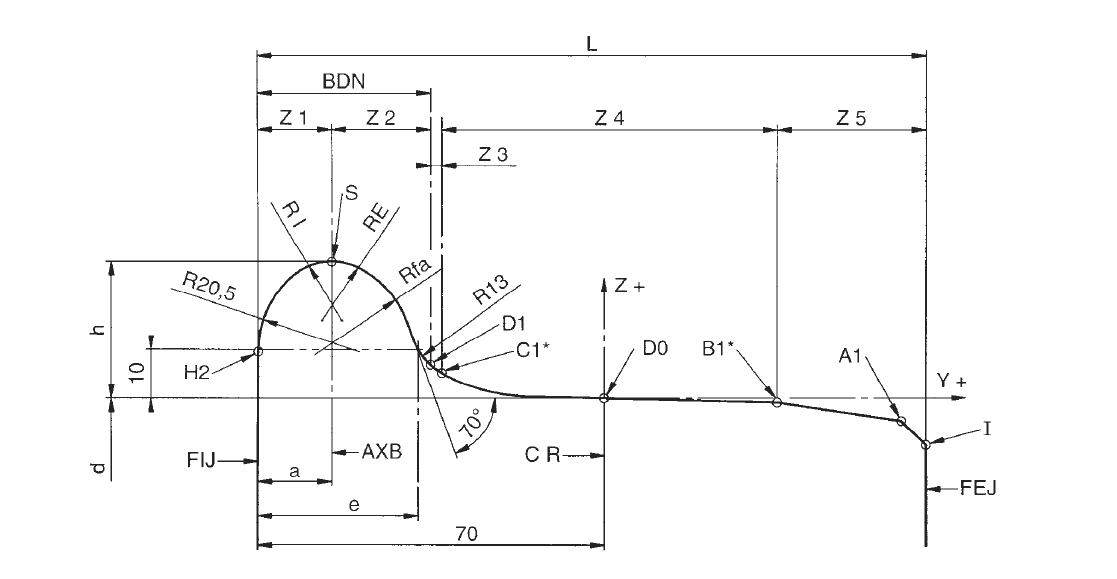
\includegraphics[width=\textwidth]{./images/wpms/uni_profile.png}
    \caption{Tread profile}
    \label{fig:uni-profile}
  \end{figure}

In the railway engineering is used to refer to wheels as \textit{wheelset}, that is a pair of wheels, fixed each other by an axle, obtaining a rotating solid (Figure \ref{fig:wheelset}). When a train is running, the two wheels belonging to the same wheelset rotate at the same speed: this is the reason why the flange is put in the inner side and the wheel is conical. During train's motion, it may happen that the wheelset is not perfectly centered with the rail, causing the wheel to hit the rail. In this case, the total motion of the wheelset is called ``winding motion''. Thanks to wheels geometry, this motion is damped gradually and rapidly, but the repeated hits wear out the profile of the wheel. The wider will be the oscillating motion, the stronger the damage to the wheel. \\
Another advantage of the conicity is when the train turns. In this case, centrifugal force pushes the wheelset to the outer side of the curve, allowing the inner wheel to rotate along a smaller diameter with respect to the outer wheel. Wheel measures reduce the number of crashing against the rail, which are, however, not null. Another way to decrease the number of these bumps is the rotation of the rails inwards. \\
All these effects greatly reduce safety during train travel, this is why an accurate and constant monitoring of the wheel status is fundamental. \\

Anyway, the great amount of detail makes the wheel reconstruction (from laser profile) a remarkably complex operation. To simplify the problem, some points of interest are usually identified (see Figures \ref{fig:uni-profile}, \ref{fig:keypoints} and \ref{fig:measures}), such as:  
  \begin{itemize}
    \item The rolling point $L_0$
    \item The flange top $S$
    \item The finishing point $H_0$ of the flange, on internal face of the wheel, and its symmetrical $Q_2$
    \item The finishing points of inner and outer faces
  \end{itemize}
Despite their simplicity, these points can provide all the measures reported in Table \ref{tab:measures}. In the same table will be also indicated some definition of interest, useful for our analysis. \\

  ~\\
  
  \begin{longtable}{|p{3cm}|c|p{8cm}|}
  \hline
  \multicolumn{1}{|c|}{\textbf{Element}}       & \textbf{Symbol} & \multicolumn{1}{c|}{\textbf{Definition}} \\
  \hline
  
  \textit{Active flange edge}                           &                 & Revolution surface comprised between two circumferences passing through the edge points $Q_1$ and $Q_2$. \\
  \hline
  \textit{Burr}                                         &                 & Metal outflow from the rolling surface to slide out. \\
  \hline
  \textit{External side of active flange edge}          & $Q_1$           & Point placed on the active face, at the radial distance of $2 mm$ from $S$ \\
  \hline
  \textit{Flange height}                                &  $h$            & Flange height, measured with respect to the tread.\\
  \hline
  \textit{Flange size}                                  & $S_d$           & Thickness measured at a radial distance of $10 mm$ from the tread.\\
  \hline
  \textit{Internal gauge}                               & $Si$            & Distance between the inner faces of the wheels of the same axle.\\
  \hline
  \textit{Internal side of the active flange edge}      & $Q_2$           & Point placed on the active face at the radial distance of $10 mm$ from the tread. \\
  \hline
  \textit{Nominal wheel diameter}                       &  $D$            & Design tread diameter. \\
  \hline
  \textit{Outboard gauge}                               & $Se$            & Distance between the active faces of the rims of the wheels of the same axle (reference points $Q_2$). \\
  \hline
  \textit{Qr quote}                                     & $Qr$            & Slope index of the active flange edge, i.e. the distance between the horizontal projections of the circumference passing from $Q_1$ and $Q_2$. \\
  \hline
  \textit{Thickness of the rim}                         & $Sc$            & Thickness measured at the rolling circle taking into account the surface roughness.\\
  \hline
  \textit{Tread}                                        &                 & Wheel circumference located at the intersection of an orthogonal plane to the wheel axis, at $70 mm$ distance from the inner face of the wheel. \\
  \hline
  \textit{Tread wear}                                   &                 & Crushing of the rolling surface, with material re-rolling towards the outer face. \\
  \hline
  \textit{Wheel diameter}                               &  $d$            & Tread diameter. \\
  \hline
  \textit{Width of rim}                                 &  $L$            & Distance between the vertical faces of the wheel rim or wheel crown. \\
  \hline
  
  \caption{Measures of interests and their definitions}
  \label{tab:measures}
\end{longtable}

  
  %\medskip
  \vfill
  
  \begin{figure}[h!]
    \centering
    \begin{minipage}[c]{.50\textwidth}
      \centering
      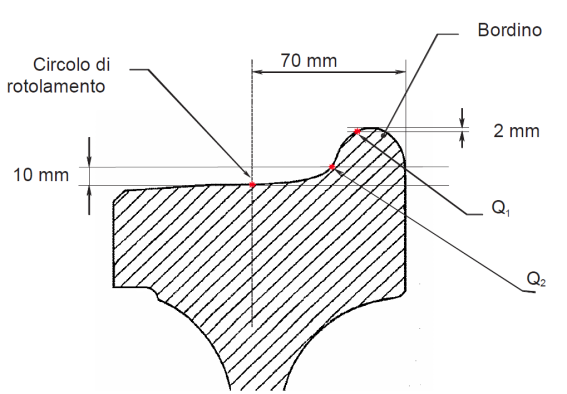
\includegraphics[width=0.95\textwidth]{./images/wpms/wheel-section.png}
        \caption{Wheel section keypoints}
    \label{fig:keypoints}
    \end{minipage}%
    \begin{minipage}[c]{.50\textwidth}
      \centering
      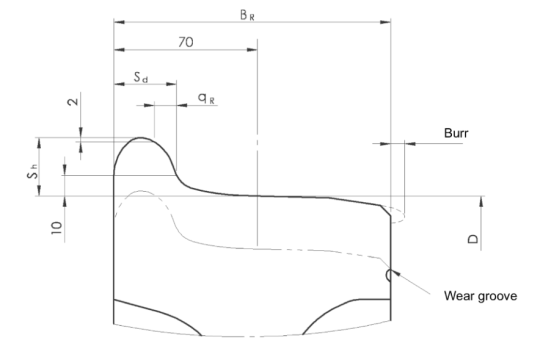
\includegraphics[width=1.05\textwidth]{./images/wpms/wheel_parameters.png}
      \caption{Wheel section measures}
      \label{fig:measures}
    \end{minipage}
  \end{figure}

  %\medskip
  \vfill

  \begin{figure}[h!]
    \centering
    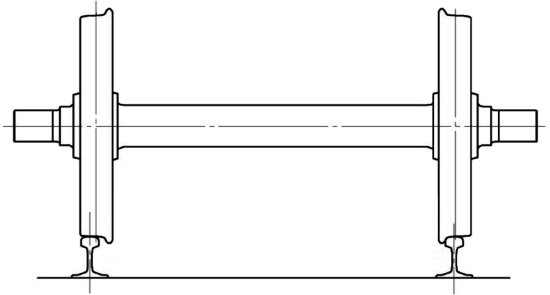
\includegraphics[width=0.7\textwidth]{./images/wpms/assile.jpg}
    \caption{Example of a wheelset}
    \label{fig:wheelset}
  \end{figure}

%  \begin{figure}[h!]
%    \centering
%    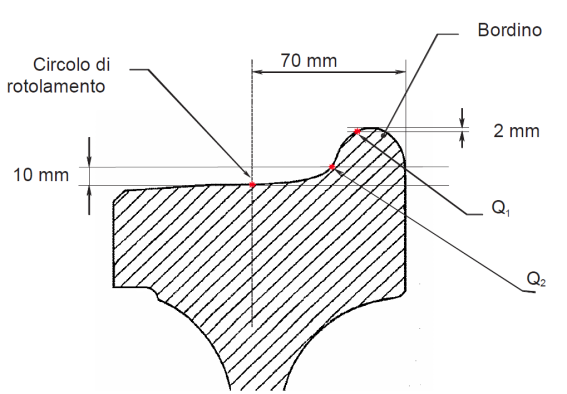
\includegraphics[width=0.6\textwidth]{./images/wpms/wheel-section.png}
%    \caption{Wheel section keypoints}
%    \label{fig:keypoints}
%  \end{figure}
%  \begin{figure}[h!]
%    \centering
%    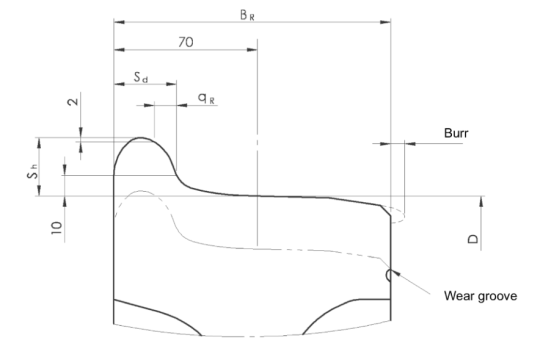
\includegraphics[width=0.6\textwidth]{./images/wpms/wheel_parameters.png}
%    \caption{Wheel section measures}
%    \label{fig:measures}
%  \end{figure}

% Needed to force next section to begin after figures
\clearpage

%%%%%%%%%%%%%%%%%%%%%%%%%%%

Wheel profile measurement system can be grouped into two categories, depending on the type of measurement, such as: \textit{static} measurement and \textit{dynamic} measurement.

In general, static measurement is performed in storage areas, during the maintenance of the train or of the wheel, when the train is stopped. This type of measures are done using mechanical calipers or optical methods: if we consider manual systems, the skill of the operator can influence seriously the results. Vice versa autonomous systems (typically based on optical sensors) are more precise and don't require any action of the operator. In both cases the main disadvantage is the fact that we have to disassemble the wheelset before performing the measures of interest, and as we said above, to achieve them periodically for each train is an impossible task.

Concerning dynamic systems, they allow to evaluate all the measures of interest while the train is running. These systems are typically based on contactless devices, such as electromagnetic or structured light sensors. Unlike mechanical sensors, these ones may also have a low resolution, but require a very good mathematical model that can process the collected data. In particular, structured light devices use at least two projector-camera pairs to avoid the problem of the occlusions. Furthermore, they need to collect at least three rolling points in different section of the profile to correctly evaluate the wheel diameter\cite{wpms-giuseppe}. Note that systems like these are more complex than the previous type: the high speeds of the trains and the serial acquisition of each axis need the presence of auxiliary technologies in order to detect the presence of a train, determine which axis is being analysed and pre-process collected data to reduce the transmission overhead. All this devices have to be synchronized if we want an high performance system. 


% Systems comparison
  \section{Systems comparison}
\label{sec:sys-cmp}
Nowadays, we can find several products on the market, developed by several companies around the world. Many of them are patented to protect the invention itself, some others are protected by corporate secrets, the remaining are available as academic publications. Commercial cameras and lasers are sufficiently powerful and accurate that the hardware could be considered negligible when we want to compare these systems. What really characterises each of them is the software, i.e. the mathematical model used to extract the wheel profile and to approximate the diameter. \\

In the following of this section, we will present some mathematical models used to evaluate the diameter of the wheels, starting from the rolling points determined by the wheels profiles. To avoid infringing patents, we will present the models without ever mentioning who the owners are. However, some of the corporations that are analysed are: % Beena Vision\footnote{ Corporation available at \url{http://www.beenavision.com/}}, Danobat\footnote{ Corporation available at \url{https://www.danobatgroup.com/en/danobat}}, Graw\footnote{ Corporation available at \url{http://www.graw.com/}}, IEM\footnote{ Corporation available at \url{http://www.iem.net/}}, KLD Labs\footnote{ Corporation available at \url{http://www.kldlabs.com/}}, MERMEC\footnote{ Corporation available at \url{http://www.mermecgroup.com/}} and MRX\footnote{ Corporation available at \url{http://www.mrxtech.com.au/}}.
  \begin{itemize}
    \item Beena Vision\footnote{\url{http://www.beenavision.com/}}
    \item Danobat\footnote{\url{https://www.danobatgroup.com/en/danobat}}
    \item Graw\footnote{\url{http://www.graw.com/en/}}
    \item IEM\footnote{\url{http://www.iem.net/}}
    \item KLD Labs\footnote{\url{http://www.kldlabs.com/}}
    \item MER MEC\footnote{\url{http://www.mermecgroup.com/}}
    \item MRX\footnote{\url{http://www.mrxtech.com.au/}}
  \end{itemize}


%%%%%%%%%%%%%%%%%%%%%%%%%%%
\subsubsection{System \#1} % BeenaVision
The first considered system uses an approach a bit different from the others. It is based on three laser-camera pairs: two are used to reconstruct the section of the wheel, while the third takes a section of the wheel parallel to its sides (perpendicular to the wheelset axis). The two sections visible from the outer side are shown in Figure \ref{fig:cmp-sys1}. In this way, line 28 allows to collect a number of points greater than three, as suggested in \cite{wpms-giuseppe}. To simplify the fitting of this last set of point on the wheel, its section is modelled as a cylinder of equation:
  \begin{equation}
    \left( y - y_0 \right) + \left( z - z_0 \right) = r^2
    \label{eq:cylinder}
  \end{equation}
instead as a cone, but this requires some corrections in order to get the exact wheel diameter. Equation \ref{eq:cylinder} is the same as a circle, whose axis passes through the center point $\left( y_0, z_0 \right)$. This equation can be solved using only three points, but it is more precise if the number of used points is greater.
  \begin{figure}[t!]
    \centering
    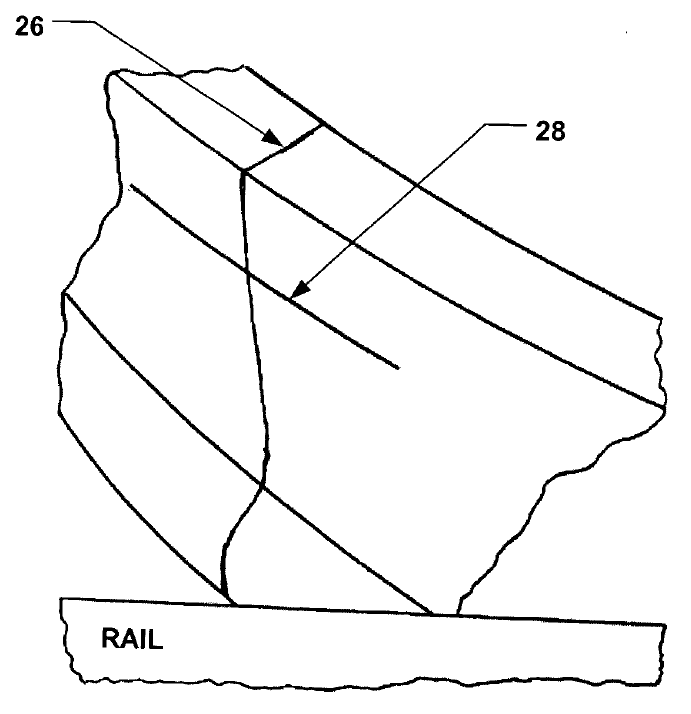
\includegraphics[width=0.6\textwidth]{./images/wpms/lasers1.png}
    \caption{System \#1, outer side collected sections}
    \label{fig:cmp-sys1}
  \end{figure}
Lasers lines are extracted from the (simultaneous) acquired images, after a preprocessing. This data elaboration consists of image resizing, laser spots detection, image equalization using threshold filters and rejection of noisy points. In particular, the detection of the laser spots is performed using edge-detection algorithms instead of subpixel filters; in this case the subpixel precision is guaranteed by the image resizing. Note that line 28 generally is not perpendicular to the axis of the wheel, because of the inclination of the same with respect to the rail. This situation introduces an error when we compute the diameter. Thus, the profile has to be projected in a plane perpendicular to the axis of the wheel, before compute the Equation \ref{eq:cylinder}. This correction is called \textit{radial compensation}. \\
The presentations of the commercial products of this corporation offer a precision greater of $96\%$ for each measure of interest (diameter, flange width and height, \ldots).

%%%
% If it is the case to do that, I've some other notes about BeenaVision
%%%


%%%%%%%%%%%%%%%%%%%%%%%%%%%
\subsubsection{System \#2} % Danobat
Differently from the previous system, this one proposes a method that can be used with many different structured light projectors, even if all proposed solutions are focused on laser stripes. This proposal basically uses at least two laser-camera pair in order to reconstruct the entire profile of the wheel, and solve the occlusion problem. \\
Once the laser spots are detected from the two different acquisitions, they are converted in a common 3D reference system, where $X$ is the longitudinal direction, $Y$ is the transverse direction and $Z$ the vertical direction. Converted data are then corrected, by aligning the profile with the ideal reference system: this corrects distortions due to the wheel inclination with respect to its axis (angle $\alpha$ and $\beta$, as shown in Figure \ref{fig:cmp-sys2}).
  \begin{figure}[t!]
    \centering
    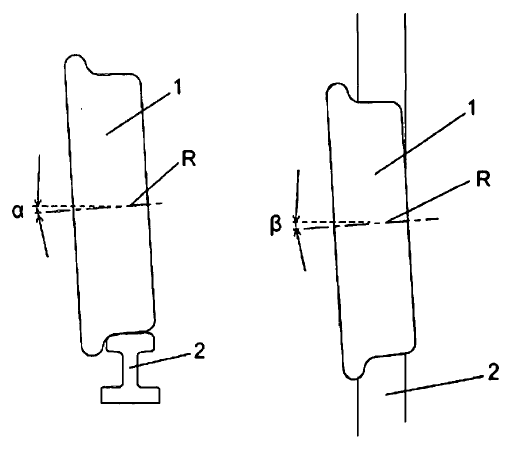
\includegraphics[width=0.7\textwidth]{./images/wpms/wheel-rotation.png}
    \caption{System \#2, wheel rotations with respect to ideal axis. $R$ is the ideal rotation axis, $1$ is the wheel and $2$ the rail.}
    \label{fig:cmp-sys2}
  \end{figure}
This is performed by correcting the rotation of the tensors parallel to the inner and outer side, with respect to the ideal ones. Furthermore this correction allows to analyse the profile in a well known position, regardless of how the profile is acquired by the camera (remember that the train is running on the sensor). At this point, for each detected laser spot, from the flange to the wheel contact surface, a radius is computed. Radius is understood as the distance between a point of light reflected on the section of the wheel and a transverse height $Y$ of the axis $R$ of the wheel, and it is computed using the equation:
  \begin{equation*}
    Radius = \sqrt{x^2 + z^2}
  \end{equation*}
where $x$ and $z$ are respectively the longitudinal and the transverse heights of each point of light of the laser line.
When all the parameters of interest are rough estimated, a Gauss-Newton algorithm is used in order to minimize the error on the computed radii, and in this way to refine the angles $\left( \alpha, \beta \right)$ and the position and orientation of each profile. At the end, the measures of interests are computed. The presentations of the commercial products of this corporation offer a precision around of $0.2 \, mm$ for measures concerning profile of the wheel (flange height and thickness, qR factor, \ldots) and a precision around of $1 \, mm$ for the diameter.
 
 
%%%%%%%%%%%%%%%%%%%%%%%%%%%
\subsubsection{System \#3} % IEM
Like the system \#2, also this approach is thought to be used both with laser beams and with structured light. Even the order with which the operations are performed is about the same:
  \begin{itemize}
    \item detection of the laser stripe;
    \item data conversion into the 3D $\left(XYZ\right)$ reference system and alignment to the ideal orientation;
    \item interpolation of the raw data using standard shape fitting algorithms;
    \item evaluation of the measures of interests.
  \end{itemize}
What distinguishes this system from others, is the approach used to detect the laser spot and to reconstruct the profile of the wheel. In fact, it uses standard geometric fitting algorithms to find each part that dial the profile, as flange, rim, wheel inner and outer sides, \ldots Once the entire profile is built from each acquired image (generally, one for each laser-camera pair used), the diameter of the wheel is determined using a standard circle fitting algorithm\footnote{Not specified in the patent} that allows to approximate the rolling circle. \\

Unfortunately, in the website of the manufacturer we have found only commercial description about the products, but no information about their precision, or accuracy. However, these informations could be meaningless. This corporation is the owner of many patents regarding laser-triangulation systems, each one of them proposes a different approach to the problem. For example, some of them are based on expert system or on neural network. Furthermore, different sensors are suggested, such as electromagnetic or acoustic devices. \\
All the patents analysed described a complete system, but avoid to study in details the algorithms used to process collected data, thus we can only speculate on how proposed systems really work.

%%%%%%%%%%%%%%%%%%%%%%%%%%%
\subsubsection{System \#4} % Mermec
Like the previous systems, also this last one is based on, at least, a couple of a laser-camera pair, that allow to reconstruct the entire profile of the wheel, similarly as shown in Figure \ref{fig:cmp-sys4}.
The laser beams are collected by the three cameras, and the spots are located using sup-pixel approximation algorithms, that increase the accuracy of the laser estimation, starting from the acquired images. Thus, the entire profile is rebuilt merging the inner and outer laser lines, and aligned to the ideal orientation. At this point, some keypoints are determined in order to evaluate the measures of interest. \\

One of the most meaningful points, is the rolling point: in fact it allows to estimate the diameter of the wheel. As in the previous case, this operation requires at least three points, taken from at least three synchronous acquisitions. Also in this case, a radial compensation is needed, in order to reduce the measurement error; if the system provides many triangulation groups, it is possible to estimate different diameters, and then average along this values. Note that, in this way it is possible to approximate the wheel circle, but it is not possible to consider wheel ovalization.
% Concerning the estimation of the diameter, given at least three different rolling points, belonging to the rebuilt profiles and taken in different positions, the Erone's formula is used:
%  \begin{equation*}
%    D = \frac{2\cdot a\cdot b\cdot c}{\sqrt{(a+b+c)(-a+b+c)(a-b+c)(a+b-c)}}
%  \end{equation*}
%where $a$, $b$ and $c$ are the sides of the triangle with vertexes the three point above. In this way it is possible to approximate the wheel circle, but it is not possible to consider wheel ovalizations.
  \begin{figure}[t!]
    \centering
    \begin{minipage}[c]{.49\textwidth}
      \centering
      %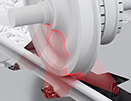
\includegraphics[width=\textwidth]{./images/wpms/mm-wpms.jpg}
      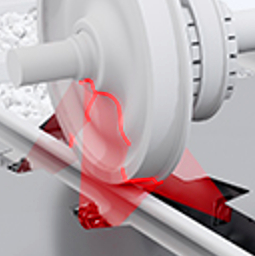
\includegraphics[width=0.8\textwidth]{./images/wpms/test2_cut.jpg}
    \end{minipage}%
    \hfill
    \begin{minipage}[c]{.49\textwidth}
      \centering
      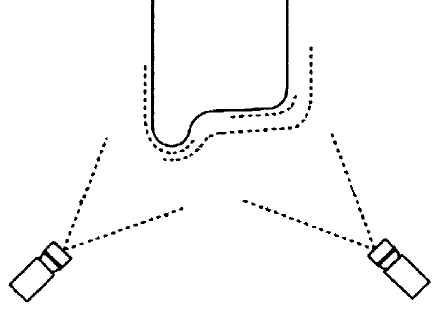
\includegraphics[width=\textwidth]{./images/wpms/laser_pts.png}
    \end{minipage}
    
    \caption{System \#4, example of system configuration.}
    \label{fig:cmp-sys4}
  \end{figure}

%%%%%%%%%%%%%%%%%%%%%%%%%%%
\subsubsection{System \#5} % \cite{wpms-giuseppe}
This last system proposes an alternative process to extract the laser stripe. Instead of improving the accuracy of the peak detection working on sub-pixel approximation, it uses an edge detector presented in \cite{chen2013efficient} and \cite{659930}. In this way, it is possible to detect the maximum of the second derivative of the grey level perpendicular to the laser stripe. Thus, it is possible to improve the peak detection even when the beam is not perpendicular to the pixel direction in the sensor, specially when the laser line bends (e.g. in the flange side). The system boast of reaching the precision of $0.1$ pieces of pixels, regardless of the variations in the width or light intensity (i.e. grey values) of the beam. Furthermore, the approach is more robust with respect to noise.

In order to correctly determine the diameter of the wheel, the system needs to rotate the profile, so that the rim plane segment can be parallel to the y-axis of the 2D coordinate frame on the laser plane. Hence, three rim plane segments can be determined, and using the 3D coordinates in the world reference system, it is possible to obtain the equation of the wheel rim plane by fitting all of the rim plane segments:
  \begin{equation}
    \pi_rim : a_rx + b_ry + c_rz + d_r = 0
    \label{eq:sys5-plane}
  \end{equation}
At the end, the diameter can be determined by projecting the flange vertexes and at least two contact points on the plane described in the Equation \ref{eq:sys5-plane}. Each of the point $p$ is projected in the rim plane accordingly with:
  \begin{equation*}
    p' = p + t\cdot\frac{N^T}{||N||}
  \end{equation*}
where $N = \begin{bmatrix} a_r, b_r, c_r \end{bmatrix}$, and $t$ is the distance from $p$ to the wheel rim plane. Thus, a maximum likelihood criterion is used against the noise, so as the approximation of the center of the wheel is improved, and a non-linear optimization method (e.g. Levenberg–Marquardt) can be performed to solve the problem. \\
The Levenberg–Marquardt algorithm (\acs{LMA} from the names of its inventors) is used to solve generic curve-fitting problems, and it always finds a local minima at least. This algorithm is slower that the Gauss-Newton one, but it is more precise. It is based on a least-squares method: given a set of $m$ empirical datum pairs $\left( x_i, y-i \right)$ of independent and dependent variables, find the parameters $\beta$ of the model curve $f(x,\beta)$ so that the sum of the squares of the deviations is minimized. \\

%%%%%%%%%%%%%%%%%%%%%%%%%%%
% Conclusion to the chapter
~\\

As we can see, the proposed systems are less than the number of the corporations analysed. As just mentioned before, many companies prefer to protect their products with corporation secrets instead using patents. Furthermore, many of the patents found are related to different systems or approaches (for example regarding static systems). These choices prevented us to comment all the products on the market. However, the systems discussed above, and summarised in Table \ref{tab:wpms:summaries}, are a good sample of the possible solutions for measuring the world using laser triangulation-based systems.
  % \caption{Summery of the systems above.}
% \label{tab:wpms:summaries}

\begin{table}[t!]
\footnotesize
\centering
\begin{tabular}{|l|p{4cm}|p{4cm}|l|}

\hline
\multicolumn{1}{|c|}{\textbf{\#}} & \multicolumn{1}{c|}{\textbf{Preprocessing}} & \multicolumn{1}{c|}{\textbf{Diameter}} & \multicolumn{1}{c|}{\textbf{Precision}} \\

\hline
\textit{1}  & * image resizing;                                                  & Profile radial                                                               & Higher than $96\%$  \\
            & * laser spots detection;                                           & compensation and                                                             &                     \\
            & * image equalization;                                              & approximation of the                                                         &                     \\
            & * rejection of noisy points.                                       & wheel to a cylinder                                                          &                     \\
			&                                                                    & instead of a cone.                                                           &                     \\
			&                                                                    &                                                                              &                     \\
			
\hline
\textit{2}  & * profiles extraction and                                          & Estimation of the center                                                     & $0.2 \, mm$ for measures \\
            & conversion in a common reference system;                           & of the wheel and computation of the radius for each                          & $1.0 \, mm$ for radius   \\
            & * profiles radial correction;                                      & rolling point. Application of a Gauss-Newton                                 &                          \\
            & * profiles merge.                                                  & algorithm to reduce the approximation error.                                 &                          \\
            &                                                                    &                                                                              &                          \\

\hline
\textit{3}  & * detection of the laser                                           & Standard circle fitting                                                      & $0.1 \, mm$ for measures \\
            & stripe;                                                            & algorithm                                                                    & $1.0 \, mm$ for radius   \\
            & * data conversion into the 3D reference system;                    &                                                                              &                          \\
            & * alignment to the ideal orientation;                              &                                                                              &                          \\
            & * data interpolation using shape fitting algorithms.               &                                                                              &                          \\
            &                                                                    &                                                                              &                          \\

\hline
\textit{4}  & * frame filtering;                                                 & Evaluation through                                                           & Not found           \\
            & * profile extraction;                                              & rolling points                                                               &                     \\
            & * conversion into 3D reference system;                             &                                                                              &                     \\
            & * profiles merge;                                                  &                                                                              &                     \\
            & * performing of radial compensation to the profile.                &                                                                              &                     \\
            &                                                                    &                                                                              &                     \\

\hline
\textit{5}  & * Profile extraction using edge detector algorithms.               & * Alignment of the profile to the reference system;                      & Not found               \\
            &                                                                    & * fitting of the wheel rim plane;                                        &                         \\
            &                                                                    & * projection of the flange on the plane;                                 &                         \\
            &                                                                    & * use of a maximum likelihood algorithm to reduce the error.             &                         \\
\hline
\end{tabular}

\caption{Summery of the systems above.}
\label{tab:wpms:summaries}
\end{table}
%  \begin{table}
%    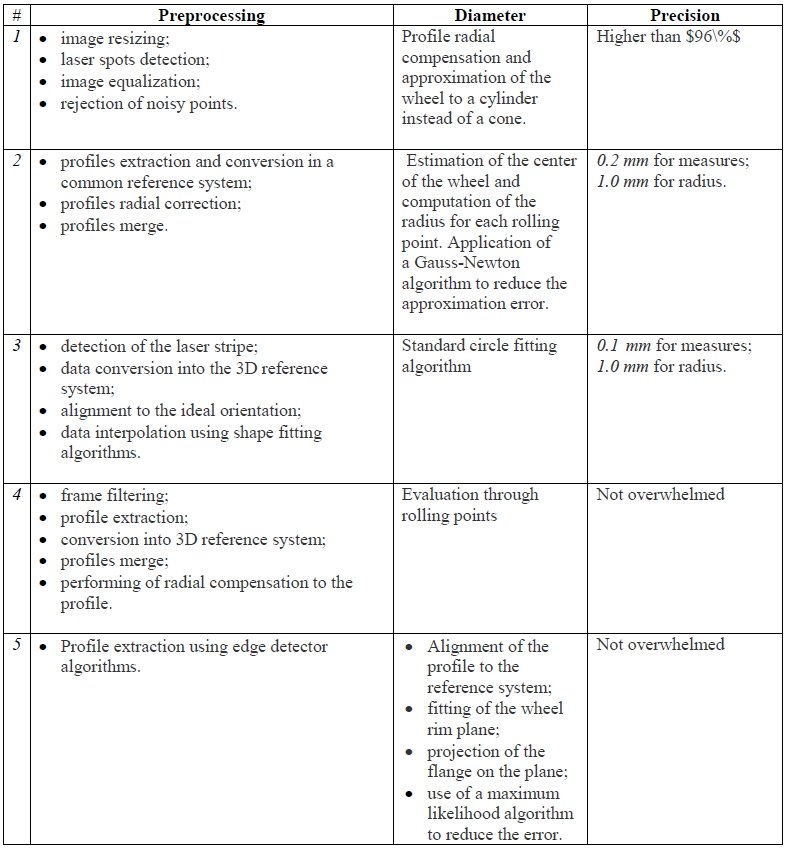
\includegraphics[width=\textwidth]{./images/wpms/tab.PNG}
%    \caption{Summery of the systems above.}
%    \label{tab:wpms:summaries}
%  \end{table}	    % Originally ch1
  \chapter{A complete error propagation model}
\label{ch::model}
%
% Original title:
%   Modello del sistema di misura per triangolazione laser-telecamera e sua caratterizzazione
% In English:
%   A complete error propagation model for laser-camera triangulation systems
%
% Presentation to the chapter
  \textit{In this chapter we will present a complete mathematical model for errors propagation in \acs{SOL} systems, and discuss its characterization and limits. Furthermore we briefly present some alternative solutions analysed.}

% Problem definition
  \section{Problem definition}
Designing a new product is a very delicate process in which we have to consider all the details of interest. The purpose of this process is to maximise the final result. The greater is the product complexity, the more this process is tricky. In the case of study, a \acs{WPMS} is rated as good if the measures made with it are close enough to the real ones. A question rises: what does ``close enough'' mean? \\

As described in Chapter \ref{ch:technology}, a \acs{SOL} system is made up of many components: cameras, sensors, lenses, laser projectors, laser-camera reciprocal positions, etc. All of these components are sources of noise. Accurately control these sources, allows to significantly increase the accuracy of the output measurement. Unfortunately this is not only a problem of noise. When we design a new system we decide how to put the elements, how to link them and which positions are the best to reach our goal, but when too many elements are taken into account at the same time, it is very difficult to estimate the effect of each single choice on the final result. When there are no models or virtual system that allow to simulate this chain of effects, the only way to evaluate the quality of the system is to build and to try it on real situation or in laboratory, with a waste of time and money in the case the system doesn't reach given requirements. Time and money are two fundamental aspects in a company, specially when products have to be customized on customer needs, or when a new product have to be designed within a deadline. \\

By combining what has just been said with \acs{WPMS}s description in Chapter \ref{ch:sys_cmp}, both from the point of view of hardware and software, we can summarize the sources of noise/error for the acquisition of images and measurement, as follows:
  \begin{itemize}
    \item Environment
      \begin{itemize}
        \item Working tolerances
        \item Temperature range
        \item Installation
        \item Vibration/Shock
        \item External light conditions
        \item Dirty and wet condition on the target (wheel surface)
      \end{itemize}
      %
    \item Not ideal of the model
      \begin{itemize}
        \item Wheel yaw and camber
        \item Laser spot shape (discussed in Subsection \ref{subsec:lenses})
        \item Lenses (discussed in Subsection \ref{subsec:peak-detection})
      \end{itemize}
      %
    \item Images acquisition process
      \begin{itemize}
        \item Laser plane
        \item System calibration and geometrical parameters evaluation
        \item Profile extraction
      \end{itemize}
      %
    \item Data processing
      \begin{itemize}
        \item Point cloud interpolation
        \item Keypoints detection
        \item Measures evaluation and error propagation (Summaries and differences, application of closed formulas, \ldots)
      \end{itemize}
  \end{itemize}


The model proposed in this chapter aims to evaluate the error made determining a 3D point in the world, starting from the detection of its projection in the image. The model tries to consider all the elements described in Chapter \ref{ch:technology}, organizing them accordingly to the \acs{SOL} systems geometry. In particular, we will focus on the problem of sub-pixel point extraction. In the end, we will try to improve the model, considering the calibration problem and including the corrections due to the non-ideality of the image acquisition. \\

In Appendix \ref{ap:model} we summarized the proposed model, with particular attention to the notation and to the simplicity of comprehension. In Appendix \ref{ap:nomen} we added a table with all the definition of interests for this chapter.


% Introduction to error propagation
  \section{Introduction to error propagation}
Before studying the model, we briefly recall some notions on propagation of measurement errors. Accordingly with \cite{book:ivm}, the size is a property of an object that could be expressed by a number and a reference, i.e. it is measurable. Physical size measurement is generally followed by the error estimation associated with it, specially when they are indirect measure. In the general case, given the function $y = f(x)$, we can generalized its error as
  \begin{equation}
    \sigma_f = \begin{vmatrix}
      \frac{df}{dx}
    \end{vmatrix}_{x = x_0}
    \sigma_x
    \label{eq:er_prop_1}
  \end{equation}
If $y = f(\bar{x})$, function of $k$ variables, Equation \ref{eq:er_prop_1} can be generalize as:
  \begin{equation}
    \sigma_f = \sum_{j = 1}^k \begin{vmatrix}
      \frac{\partial f}{\partial x_j}
    \end{vmatrix}_{x = x_0}
    \sigma_x
    \label{eq:er_prop_2}
  \end{equation}
The propagation of the maximum errors by using the differential, is based on the assumption that infinitesimal variations of the variables are given by the respective errors. If we want to estimate the maximum error for $y$, it is appropriate to sum up all the terms consistently, i.e. taking the partial derivative modules.


% Triangulation system geometry
  \section{Triangulation system geometry}
\label{sec:init-modelanalysis}
At first, we analyse the errors due to the geometry of the triangulation system. For simplicity, we will focus on the standard geometry (described in Section \ref{sec:lctt}): the analysis for other geometries is trivial. \\

As illustrated in Figure \ref{fig:laser-triang}, the laser-camera pair form a triangle with angle $\phi$ between the baseline (the plane along the distance between the laser and the camera), and the optical axis of the camera. In \acs{SOL} systems, $\phi$ is
\clearpage
  \begin{figure}[h]
    \centering
    \begin{minipage}[c]{\textwidth}
      \centering
      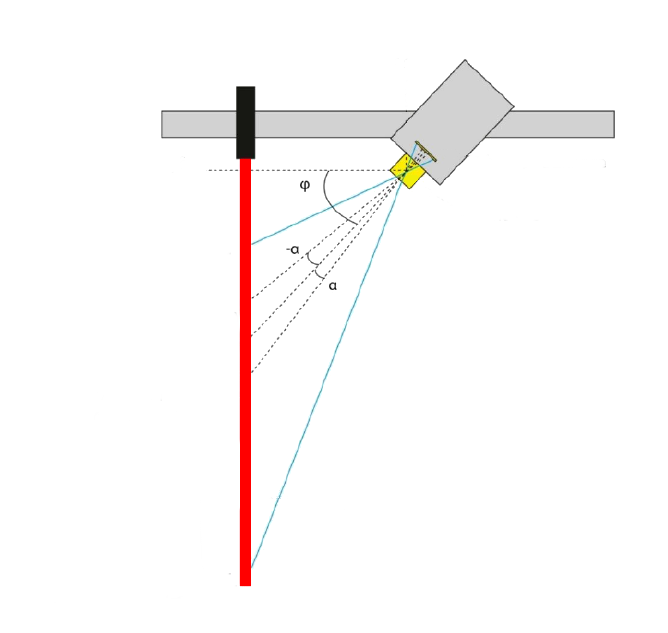
\includegraphics[width=0.7\textwidth]{./images/model/laser_triang.png}
      \caption{\acs{FOV} and characteristic angles}
      \label{fig:laser-triang}
    \end{minipage}
    \vfill
    \begin{minipage}[c]{\textwidth}
      \centering
      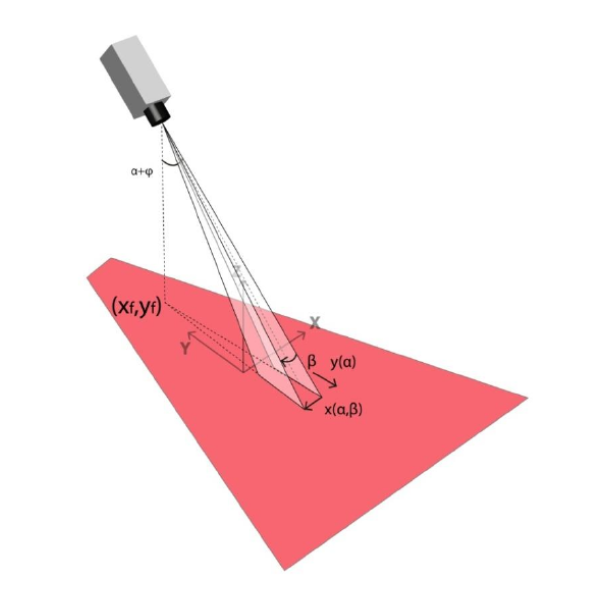
\includegraphics[width=0.7\textwidth]{./images/model/laser_triang_pdv.png}
      \caption{Angles definitions}
      \label{fig:laser-triang-pdv}
    \end{minipage}
  \end{figure}
\clearpage \noindent
called \textit{triangulation angle}. If $\phi$ and the baseline are known, any point in the 3D space belonging to the laser plane, is located estimating the offset $\alpha$ with respect to $\phi$, and the offset $\beta$ with respect to the optical axis of the camera. Accordingly with \cite{th:quattrini}, and using simple mathematical relations, we can locate the $y$ coordinate as function of the angle $\alpha$ as follows:
  \begin{equation}
    \label{eq:model-ya}
    y\left( \alpha \right) = y_f + z_f \tan \left( \phi + \alpha \right)
  \end{equation}
where $\left( x_f, y_f, z_f \right)$ are the principal point projection coordinates in the laser plane (in the world reference system), as shown in Figure \ref{fig:laser-triang-pdv}. Note that using this notation, $z_f$ is the distance from the laser to the camera, previously called baseline. \\

Now let's look at the Figure \ref{fig:laser-triang-pdv}. As mentioned at the end of the Section \ref{sec:lctt}, camera's resolutions varies changing the distance of the target from the camera. In particular this is true for the resolution along the laser line (axis $x$ with respect to out notation). Points having the same $x$ coordinates but different $y$ are estimated with different camera resolutions. This means that the values of $x$ strongly depends on the angle $\beta$ (that identify the value of $x$ with respect the the optical axis of the camera), but also on the angle $\alpha$ (that identifies the value of $y$ with respect to the triangulation angle). For these reasons we can write
  \begin{equation}
  \label{eq:model-xab}
    x(\alpha, \beta) = \frac{y\left( \alpha \right) - y_f}{\sin(\phi + \alpha)}\tan(\beta)
  \end{equation} \\
As we can see, $x$ strongly depends on $y$, accordingly with what we said in Section \ref{sec:lctt}, about the trapezoidal shape of the laser plane. Still for the shape of the laser, a similar consideration can be made for the $y$ coordinate, because of the trapezoidal shape of the laser plane.
% To be precise, a similar consideration can be made for the $y$ coordinate, because of the trapezoidal shape of the laser plane.
However, in this case the differences between the nearest and the farthest \acs{FOV}s along the $x$ axis, are negligible. For theses reasons we will consider Equation \ref{eq:model-ya} as a good approximation of the relation between $y$ and $\alpha$. \\

Accordingly with what we said in Section \ref{sec:teo-calibration}, during calibration phase the choice of the reference system is arbitrary, so we can put $\left( x_f, y_f, z_f \right) = \left( 0, 0, z_f \right)$ without loss of generality. In this way, Equations \ref{eq:model-ya} and \ref{eq:model-xab} can be simplified. \\

At this point it is easy to estimate the error associated with the two newly introduced measures. Applying the simplification, for Equation \ref{eq:model-ya} we can write:
  \begin{equation}
    \label{eq:model-ya-err0}
    \sigma_{y_\alpha} = \sqrt{
      \left( \frac{\partial y}{\partial z_f} \right)^2 \sigma_{z_f}^2 +
      \left( \frac{\partial y}{\partial \phi} \right)^2 \sigma_\phi^2 +
      \left( \frac{\partial y}{\partial \alpha} \right)^2 \sigma_\alpha^2
    }
  \end{equation}
while for Equation \ref{eq:model-xab} we can write
  \begin{equation}
    \label{eq:model-xab-err0}
    \sigma_{x\left( \alpha, \beta \right)} = \sqrt{
      \left( \frac{\partial x}{\partial \phi} \right)^2 \sigma_\phi^2 +
      \left( \frac{\partial x}{\partial \alpha} \right)^2 \sigma_\alpha^2 +
      \left( \frac{\partial x}{\partial \beta} \right)^2 \sigma_\beta^2
    }
  \end{equation}\\
In these last equations, the $\sigma$ are the errors committed evaluating each component in the Equations \ref{eq:model-ya} and \ref{eq:model-xab}. As we can see, in Equations \ref{eq:model-ya-err0} and \ref{eq:model-xab-err0} we are considering also $\phi$ and $z_f$ that are constructive parameters that depend on the accuracy with which the system was built or installed. Typically, these parameters are corrected thanks to the calibration process, that allows to estimate camera intrinsic and extrinsic parameters, as mentioned in Section \ref{sec:teo-calibration}. In addition, the calibration process uses many algorithms that in turn use different heuristics to estimate camera parameters. This means that all parameters are affected by error, but as we can see later, we can consider these errors negligible. So we can simplify Equations \ref{eq:model-ya-err0} and \ref{eq:model-xab-err0} respectively as follows
  \begin{equation}
    \label{eq:model-ya-err1}
    \sigma_{y_\alpha} = \sqrt{
      \left( \frac{\partial y}{\partial \alpha} \right)^2 \sigma_\alpha^2
    }
  \end{equation}
  
  \begin{equation}
    \label{eq:model-xab-err1}
    \sigma_{x\left( \alpha, \beta \right)} = \sqrt{
      \left( \frac{\partial x}{\partial y_\alpha} \right)^2 \sigma_{y_\alpha}^2 +
      \left( \frac{\partial x}{\partial \alpha} \right)^2 \sigma_\alpha^2 +
      \left( \frac{\partial x}{\partial \beta} \right)^2 \sigma_\beta^2
    }
  \end{equation} \\

Keeping focus on the geometry of the system, the second element to consider is the laser plane. In standard geometry, variations on laser pitch and roll rotations, with respect to the reference system, can affect heavily the final measure. By trigonometry we know that by changing the angle, the point projections also change in the two axes of the reference system. The same effect is present when we rotate the laser plane with respect to the $x$ axis (roll) or with respect to the $y$ axis (pitch). These errors are more apparent in the other triangulation geometries. What we have to do, is to compensate these rotations projecting the laser plane on the ideal one. The compensations are performed as follows:
  \begin{equation}
    \begin{matrix}
      y_w = y(\alpha) \cdot cos(\rho) \\ ~ \\
      x_w = x(\alpha, \beta) \cdot \cos(\gamma)
    \end{matrix}
    \label{eq:radial-compensations}
  \end{equation} \\
where $\rho$ is the laser roll angle, and $\gamma$ is the laser pitch angle. Using the model introduced in Equation \ref{eq:er_prop_2}, we can write, respectively:
  \begin{equation}
    \sigma_{y_w} = \sqrt{
      \left( \frac{\partial y_w}{\partial y(\alpha)} \right)^2 \sigma_{y_\alpha}^2
      + \left( \frac{\partial y_w}{\partial \rho} \right)^2 \sigma_\rho^2
    }
    \label{eq:err-radial-comp-yw}
  \end{equation}
  \begin{equation}
    \sigma_{x_w} = \sqrt{
      \left( \frac{\partial x_w}{\partial x\left( \alpha, \beta \right)} \right)^2 \sigma_{x\left( \alpha, \beta \right)}^2 +
      \left( \frac{\partial x_w}{\partial \gamma} \right)^2 \sigma_\gamma^2
    }
    \label{eq:err-radial-comp-xw}
  \end{equation} \\
where $\sigma_{y_\alpha}$ and $\sigma_{x\left( \alpha, \beta \right)}$ are the ones evaluated in Equations \ref{eq:model-ya-err1} and \ref{eq:model-xab-err1} respectively. \\

A practical example in which these compensations are needed, is the \acs{WPMS}. In autonomous \acs{WPMS}s placed alongside the rails, specular geometry is generally used, and wheels are measured while the train is running. In these cases we are not sure to measure the wheel exactly along its axis, so the acquired profiles have to be compensated. This type of correction is called \textit{radial compensation}. \\
% The errors due to non-ideality of laser plane placement can be seen also as non-ideality of work conditions. In autonomous \acs{WPMS}s placed alongside the rails, specular geometry is generally used, and wheels are measured while the train is running. In these cases we are not sure to measure the wheel exactly along its axis, and typically corrections like the ones for rolls are needed. In these field, these corrections are referred as \textit{radial compensation}. \\
We can consider the same things about pitch. Sometimes the wheel under analysis is not perpendicular with the laser plane, because wheel yaw and camber. Also in these cases $x$ values must be compensated.

%We can see here, the determination of $x$ is fully dependent by the formulation on $y$.


% Word to camera discretization
  \section{World to image plane}
\label{sec:wrd2cam}
Accordingly with what we reported in Section \ref{sec:pinhole_camera}, the second step is to determine the 3D point coordinates in a reference system concordant with the image plane. The plane of interest $S$ is a plane parallel with lens plane and passing through the plane parallel to the sensor.  This choice is due to the possibility to tilt the lens with respect to the sensor, accordingly with the Scheimpflug principle, described above. If we consider the image plane parallel to the sensor directly, some issue arises. Tilting the lens changes the focal length of the camera, that varies point by point, resulting in a distorted image. This problem can be simplified observing that if we tilt the lens, we add an image plane rotated with respect to the classical image plane. In this way, the transformation between the two planes is a simple projection between planes. So we decided to split the problem in two subproblems: the first, described in this section, requires to change coordinates reference system; the second, described in Section \ref{sec:scheimflug}, needs to project the point on a different plane. Furthermore, this choice allows to simplify the mathematical model. \\

Let's focus on the Figure \ref{fig:laser-triang-a}.
  \begin{figure}[t!]
    \centering
    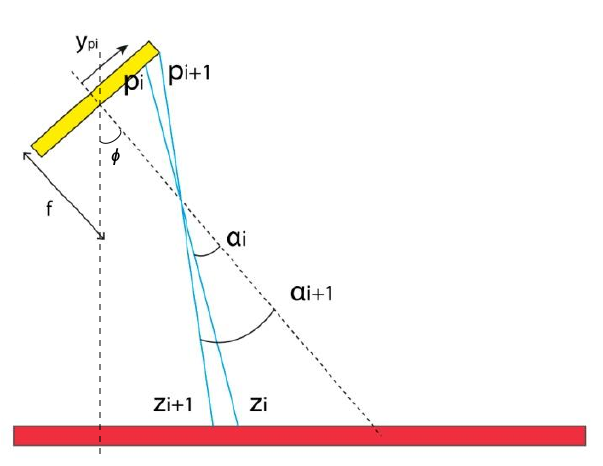
\includegraphics[width=0.7\textwidth]{./images/model/laser_triang_alpha.png}
    \caption{World to image plane}
    \label{fig:laser-triang-a}
  \end{figure}
As we can see, a change in the 3D point coordinates causes a variation in the image plane. However this alterations deals with the angle $\alpha$, estimated as offset from the triangulation angle $\phi$. Furthermore, laser plane and image plane are not parallel: this means that the two variations are different. What we are interested in, is the variation on the image plane, not in the world, so we can formulate this problem, accordingly with \cite{th:quattrini}, as:
  \begin{equation}
  	\alpha_i = \arctan\left( \frac{y_{s_i}}{f} \right)
    \label{eq:model:alpha}
  \end{equation}
where $y_{s_i}$ is the $i^{th}$ points in the image plane $S$. Being careful, it is simple to observe that the same relation is valid when determining the error due evaluating the $x$ coordinate, but with respect to the optical axis:
  \begin{equation*}
  	\beta_i = \arctan\left( \frac{x_{s_i}}{f} \right)
  \end{equation*}
Note that this step is important also to determine the natural camera resolution, in fact it allows to define the minimum variation appreciated by the sensor while it is observing the world.

So we can conclude writing that:
  \begin{equation}
    \label{eq:det_a}
  	\sigma_{\alpha_i} = \sqrt{
  	  \left( \frac{\partial \alpha_i}{\partial y_{s_i}} \right)^2 \sigma_{y_{s_i}}^2
  	  + \left( \frac{\partial \alpha_i}{\partial f} \right)^2 \sigma_f^2
  	}
  \end{equation} \\

Also in this case, $f$ is a parameter estimated thanks to the calibration processes, so we can consider it as negligible. Then, we can simplify Equation \ref{eq:det_a} as
  \begin{equation*}
  	\sigma_{\alpha_i} = \sqrt{
  	  \left( \frac{\partial \alpha_i}{\partial y_{s_i}} \right)^2 \sigma_{y_{s_i}}^2
  	}
  \end{equation*}
The same conclusions can be applied to $\beta_i$. \\

As we will see later, this transformation is the most delicate one, probably because of the change of reference system. In fact we can consider it as a passage from 3D to 2D reference system.


% Scheimpflug geometry
  \section{Scheimpflug geometry}
\label{sec:scheimflug}
As introduced in the previous section, now, we describe the plane correction due to the application of Scheimpflug principle, tilting the lens. \\

Tilting lenses causes a variation of the image plane, which rotates to stay parallel to the lens itself. Many works, such as \cite{inproc-lens-inc}\cite{Louhichi2006}\cite{4059344}, tried to improve the calibration processes, introducing different corrections in order to balance the effects introduced by lens tilt. For the most part, they have tried to apply different rotations to the plane, but these have been shown to work only for small angles. For big angles, the rotations are not enough. \\

Consider the two image planes, the one parallel to the sensor and the tilted one: as shown in Figure \ref{fig:scheimpflug-line}, the origin of the two planes is the same, since the parallel plane can be arbitrarily placed.
  \begin{figure}[t!]
    \centering
    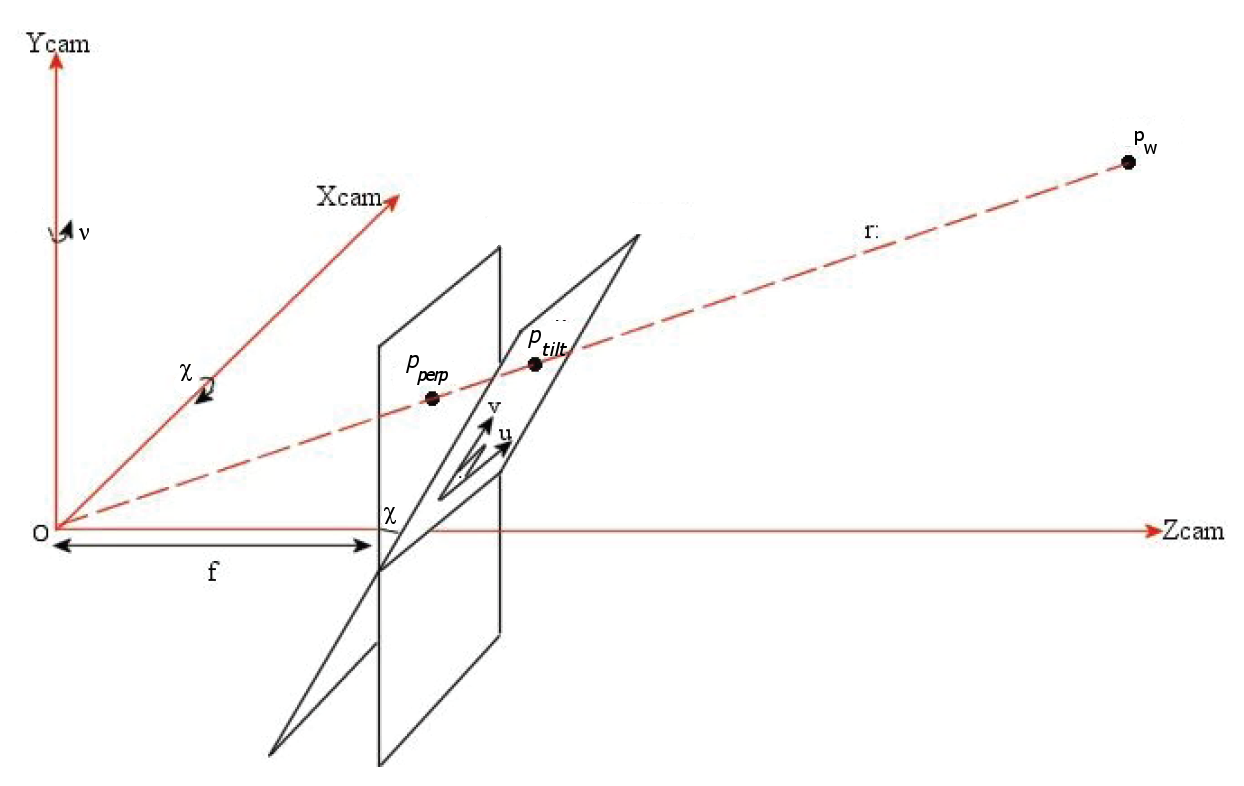
\includegraphics[width=\textwidth]{./images/model/scheimpflug.png}
    \caption{Intersection of the point in the real world in the tilted plane and in the perpendicular plane.}
    \label{fig:scheimpflug-line}
  \end{figure}
Similar to what is shown in the Figure \ref{fig:perspective_projection}, we can draw a line $r$ from the optical center $O$ to the point $p_w = \left( x_w, y_w, z_w \right)$ in the world. Accordingly with the sections above, $p_w$ is a point belonging to the laser plane, without considering radial compensation, and the tilted plane is the one in which we have projected $p_w$ in Section \ref{sec:wrd2cam}. Accordingly with \cite{SchCameraCalib}, the line $r$ passes through the two planes, allowing the definition of a system of equations that solve the intersection problem. The solution of this system can be written as follows:

  \begin{equation*}
      x_p = \lambda \cdot \left( x_s \cdot \cos\chi + y_s \cdot \sin\upsilon\cos\chi \right)
  \end{equation*}
  \begin{equation*}
    y_p = \lambda \cdot y_s \cdot \cos\upsilon
  \end{equation*}
where $\left( x_p, y_p\right) = p_{perp}$ in the figure, and $\left( x_s, y_s\right)$ ($p_{tilt}$ in figure) are the coordinate of the point in the sensor reference system, introduced in the section above. The parameter $\lambda$ is the plane coefficient and it is:
  \begin{equation*}
    \lambda = \frac{f}{f + x_s \sin\chi + y_s \sin\upsilon\cos\chi}
  \end{equation*}
The angles $\chi$ and $\upsilon$ are the swing and tilt angle of the lens, respectively. In literature, the term swing refers to a rotation with respect to the $x$ axis, while tilt refers to a rotation with respect to the $y$ axis. \\

The equation considered has been defined in a proposal for an algorithm for camera calibration. Despite that, the model capability to consider point projections gives to it a big advantage over simple rotations: the fact that we are able to consider also perspective distortions, as we have done in Section \ref{sec:pinhole_camera} for world to camera coordinate systems transformations. Note that also in this case, the $x$ coordinates are function of the $y$ ones. \\

From an analytical point of view, this is the most delicate step. The big number of elements to consider makes this calculation a big source of error. The error propagation model suggests to compute

  \begin{equation*}
    \sigma_{x_{s_i}} = \sqrt{
      \left( \frac{\partial x_{s_i}}{\partial y_{p_i}} \right)^2 \sigma_{y_{p_i}}^2 +
      \left( \frac{\partial x_{s_i}}{\partial x_{p_i}} \right)^2 \sigma_{x_{p_i}}^2 +
      \left( \frac{\partial x_{s_i}}{\partial \upsilon} \right)^2 \sigma_\upsilon^2 +
      \left( \frac{\partial x_{s_i}}{\partial \chi} \right)^2 \sigma_\chi^2
    }
  \end{equation*}
  \begin{equation*}
    \sigma_{y_{s_i}} = \sqrt{
      \left( \frac{\partial y_{s_i}}{\partial y_{p_i}} \right)^2 \sigma_{y_{p_i}}^2 +
      \left( \frac{\partial y_{s_i}}{\partial x_{p_i}} \right)^2 \sigma_{x_{p_i}}^2 +
      \left( \frac{\partial y_{s_i}}{\partial \upsilon} \right)^2 \sigma_\upsilon^2 +
      \left( \frac{\partial y_{s_i}}{\partial \chi} \right)^2 \sigma_\chi^2
    }
  \end{equation*} \\
  
\noindent
Even in this case we could ignore the contribution of the focal length, because it is a parameter estimated by the calibration process.\\

To complete this model, we should take into account also focal length and image center transformations. Reference \cite{SchCameraCalib} suggests the following set of relations:
  \begin{equation*}
    f' = \frac{f}{\cos\upsilon}
  \end{equation*}
  \begin{equation*}
    C_x' = C_x + f\cdot n_x \cdot \sin\upsilon
  \end{equation*}
  \begin{equation*}
    C_y' = C_y + f\cdot n_y \cdot \sin\chi
  \end{equation*} \\
However, our tests (described below) demonstrated that these corrections are useless. Calibration algorithms that do not implement this type of heuristics, will implement parameters (i.e focal length and optical center) optimization methods anyway, that try to evaluate these parameters as precisely as possible. The methods seem to be accurate enough to ignore the latter passages, in favour of ones suggested by the calibration.


% Lens distortion
  \section{Lens distortion and point discretization}
\label{sec:model-lens-distortion}
In Section \ref{subsec:lenses} we have introduced lenses, highlighting their advantages over the pinhole. We also introduced the differences between the thin lens model and the thick lens one, observing how, in both cases, curvature radii could introduce aberrations on the acquired image.

As we said in Section \ref{sec:teo-calibration}, all the calibration algorithms try to solve this problem, but most of them, like Tsai and Zhang, are limited to considering radial distortions. In fact it can be shown that tangential contributions are typically negligible, while radial ones increase when focal length decreases. Fortunately, in literature there are some studies about lenses and thin prism distortions, such as \cite{brown},\cite{DBLP:journals/corr/cs-CV-0308003} and \cite{Heikkila}, which offer some solutions to extend the analysis beyond this limit. \\

As a first thing, we focused on \cite{TsaiTvLenses}. Accordingly with it, the commonly used polynomial for radial distortion model, is given by the series
  \begin{equation}
    \label{eq:radial-tot}
    r_d = r + \delta_r = r + \sum_{j=1}^\infty k_jr^{(2j)}
  \end{equation}
where $r$ is the lens radius and $k_j$ is the radial coefficient of degree $j$. As we will discuss later, the used calibration algorithm are limited to the second order, so Equation \ref{eq:radial-tot} can be reduced as:
  \begin{equation}
    \label{eq:radial-2}
    r_d = r + k_1r^2 + k_2r^4
  \end{equation}

Applying Equation \ref{eq:radial-2} to distorted points, we found a simple relation, similar to that in \cite{TsaiTvLenses}:
  \begin{equation}
    \label{eq:dist-coords}
    x_{p_i} = x_{p_i}^{d} \left( 1 + k_1r^2 \right) \qquad
    y_{p_i} = y_{p_i}^{d} \left( 1 + k_1r^2 \right)
  \end{equation}
where $\left( x_{p_i}^{d}, y_{p_i}^{d} \right)$ are the distorted coordinates in the parallel to sensor image plane. In this way, we can determine the projection of a 3D point in a plane parallel to the sensor and distortion free. Note that, given a specific point, it does not make sense to consider the whole radius $r$ of the lens, so it is preferable to consider its distance from the point to the optical center (that ideally is locate in the center of the lens). \\
As we have done in previous sections, the error is propagated as follows
  \begin{equation}
    \label{eq:sigma-dist}
    \begin{matrix}
      \sigma_{x_{p_i}} = \sqrt{
        \left( \frac{\partial x_{p_i}}{\partial x_{p_i}^d} \right)^2 \sigma_{x_{p_i}^d}^2
        + \left( \frac{\partial x_{p_i}}{\partial k_1} \right)^2 \sigma_{k_1}^2
      }
      \\~\\
      \sigma_{y_{p_i}} = \sqrt{
        \left( \frac{\partial y_{p_i}}{\partial y_{p_i}^d} \right)^2 \sigma_{y_{p_i}^d}^2
        + \left( \frac{\partial y_{p_i}}{\partial k_1} \right)^2 \sigma_{k_1}^2
      } 
    \end{matrix}
  \end{equation}
Note that this transformation is the same for both $x$ and $y$, thanks to lens radial distortion symmetry. \\

At this point we have noticed that it is very easy to spread the solution to the tangential distortions. Accordingly with \cite{Heikkila} we observed that Equations \ref{eq:radial-2} could be extended easily:
  \begin{equation*}
    \mathcal{F}\left( r, \bar{k}, \bar{p} \right) = 
    \begin{bmatrix}
      x_{p_i}\left( \sum_{j=1}^\infty k_jr^{2j} \right) + \left( 2 p_1 x_{p_i} y_{p_i} + p_2 \left( r^2 + 2 x_{p_i}^2  \right) \right) \left( 1 + p_3 r^2 + \ldots  \right)
      \\
      y_{p_i}\left( \sum_{j=1}^\infty k_jr^{2j} \right) + \left(  p_1 \left( r^2 + 2 y_{p_i}^2  \right) + 2 p_2 x_{p_i} y_{p_i} \right) \left( 1 + p_3 r^2 + \ldots \right)
    \end{bmatrix}
  \end{equation*}
As we can see, to consider tangential distortion some additive factors are needed. The analysis for error propagation is the same as that for the Equation \ref{eq:sigma-dist}, but we have to pay attention to include the partial derivatives of the tangential coefficients. \\
To complete the analysis, we have done some test using nominal lens parameters given by the manufacturer, and we observed that the error improvement was negligible. \\

In the last two cases we could ignore the components depending by distortion coefficients, that we can consider correct thanks to calibration processes. \\

Looking around, we have found another model that we considered of interest. Accordingly with \cite{DBLP:journals/corr/cs-CV-0308003}, radial distortions could be formulated as a rational distribution like:
  \begin{equation*}
    \mathcal{F}\left( r, \bar{k}, \bar{p} \right) = \frac{1 + k_1r + k_2r^2}{1 + k_3r + k_4r^2 + k_5r^3}
  \end{equation*}
It is easy to derive many other formulas from the general one, and the most interesting are shown in Table \ref{tab:dist-funcs}.
  \begin{table}[t!]
  \centering
  \begin{tabular}{r|l}
  \multicolumn{1}{c|}{\textbf{\#}} & \multicolumn{1}{c}{\textbf{$\mathcal{F}\left( r, \bar{k} \right)$}} \\
    \hline
    1	& $1 + k_1 r$ \\
    2	& $1 + k_1 r^2$ \\
    3	& $1 + k_1 r + k_2 r^2$ \\
    4	& $1 + k_1 r^2 + k_2 r^4$ \\
    5	& $1 / (1 + k_1 r) $ \\
    6	& $1 / (1 + k_1 r^2)$ \\
    7	& $(1 + k_1 r) / (1 + k_2 r^2)$ \\
    8	& $1 / (1 + k_1 r + k_2 r^2)$ \\
    9	& $(1 + k_1 r) / (1 + k_2 r + k_3 r^2)$ \\
    10	& $(1 + k_1 r^2) / (1 + k_2 r + k_3 r^2)$ \\
    \hline
  \end{tabular}
  
  \caption{Polynomial and rational distortion functions}
  \label{tab:dist-funcs}
\end{table}
All these functions enjoy some properties,. in fact they are:
  \begin{itemize}
    \item radially symmetric around the center of distortion;
    \item expressed in terms of the radius $r$ only;
    \item continuous and $r_d = 0$ iff $r = 0$;
    \item the approximation of $x_d$ is an odd function of $x$.
  \end{itemize}
The above three properties act as the criteria to be good candidates as radial distribution functions. Despite that, we can see that Equation \#4 is very closed to the Equation \ref{eq:radial-2}. Furthermore, the calibration algorithms we have used are limited to second degree, and in this conditions many of these equations can be traced back to \#4. At the end, it can be shown that the performances of the remaining functions are comparable with \#4. \\
For all these reasons, we focused only on Equations \ref{eq:dist-coords}, but as we have shown in this section, it is easy to extends it to tangential distortion or to increase its degree.

\bigskip
Once we have determined the distorted point in the image plane, the last step is the point discretization. In this phase we are interested in projecting the undistorted point in the distorted sensor plane. Accordingly with \cite{TsaiTvLenses}, this projection can be performed by centering the coordinate reference system in the optical center estimated during calibration processes, and by normalizing the point value in the sensor pixel range. At the end we can write:
  \begin{equation*}
    x_{p_i}^d = d_x'(x_{c_i} - c_x) \qquad \qquad y_{p_i}^d = d_y'(y_{c_i} - c_y)
    % \label{eq:discrete-coords}
  \end{equation*} \\
where $(c_x, c_y)$ is the optical center, and $(d_x', d_y')$ the normalized pixel center to center distance, along $x$ and $y$ axis, respectively. Consistent with what we have done so far, we can conclude with error propagation:
  \begin{equation}
    \begin{matrix}
    %
    \sigma_{x_{p_i}^d} = \sqrt{
      \left( \frac{\partial x_{p_i}^d}{\partial x_{c_i}} \right)^2 \sigma_{x_{c_i}}^2
      + \left( \frac{\partial x_{p_i}^d}{\partial c_x} \right)^2 \sigma_{c_x}^2
    }
  %\end{equation*}
  \\
  %\begin{equation*}
    \sigma_{y_{p_i}^d} = \sqrt{
      \left( \frac{\partial y_{p_i}^d}{\partial y_{c_i}} \right)^2 \sigma_{y_{c_i}}^2
      + \left( \frac{\partial y_{p_i}^d}{\partial c_y} \right)^2 \sigma_{c_y}^2
    }
    %
    \end{matrix}
    \label{eq:model:err:disc}
  \end{equation} \\

\bigskip
Before concluding this section, we want to emphasize a possible source of ambiguity in understanding this model. The explanation started from the end of the chain and follows until the beginning. This choice was taken to better identify, for each step, the elements to analyse, and from which each relation depends. In this way the error determination was easy. However, we have to notice that we want to determine the error committed evaluating the point in the world, starting from pixel detection in the image, then formulas have to interpret in this sense, from pixel to world.

  
% Laser peaks detection
  \section{Laser peaks detection}
\label{sec:laser-peaks}

Starting from the point $ p_w = \left( x_w, y_w, z_w \right)$ in the 3D space, we reached its projection $p_c = \left( x_c, y_c \right)$ in the sensor reference system. At this point, the error committed while locating the peak, now depends by the technique used. \\

If we consider the general case, without using any sub-pixel approximation, the peak will be consider in the center of the pixel, i.e. located in $p_c$. Accordingly with \cite{th:quattrini}, we can model the distribution of all the possible positions of the peak along a specific direction as a \textit{uniform distribution}, centered in $p_c$, thus we can evaluate the location error with the standard deviation of the distribution, that is
  \begin{equation*}
    \sigma_{p_c} = \sqrt{\frac{\left(b - a\right)^2}{12}}
  \end{equation*}
with $a$ and $b$ the extremes of the range. \\
Let's consider the laser in its coordinates reference system. The use of a line lens allows us to spread the spot energy along a line. From a physical point of view, the signal we obtained in this way, is continuous along the direction of the abscissa, while from a mathematical point of view, the laser can be modelled as a solid Gaussian, like the one shown in Figure \ref{fig:mod-laser-line}.
  \begin{figure}[t!]
    \centering
    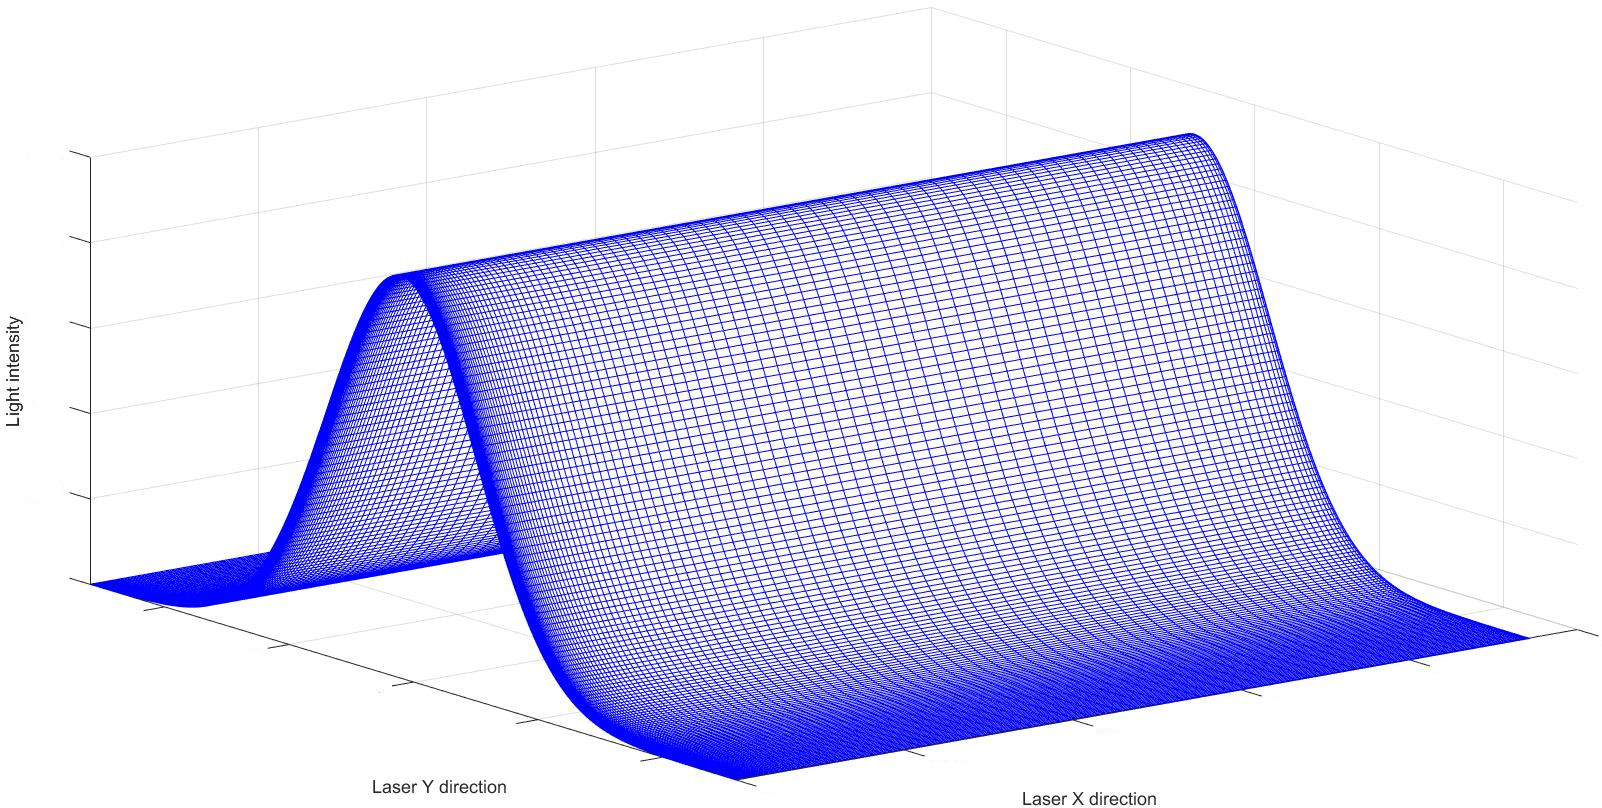
\includegraphics[width=0.8\textwidth]{./images/model/3Dgauss_grid.jpg}
    \caption{3D model of the laser line}
    \label{fig:mod-laser-line}
  \end{figure}
As we can see, we haven't any information about the position of the laser spot along the abscissa, so the only way to estimate the committed error is to use the distribution above. Thus, we modelled our error as follows:
  \begin{equation*}
    \sigma_{x_{c_i}} = \sqrt{\frac{\left(pixel \,\, size \right)^2}{12}}
  \end{equation*}
where the $pixel \,\, size$ is the ideal size of the pixel (along the $x$ axis if we assume it rectangular shaped). \\

A similar analysis can be made along the ordinate. However, even in conditions like the one shown in Figure \ref{fig:mod-laser-line}, along the ordinate we have always some informations about the shape of the laser line. This suggested us that it should be possible to consider all the mathematical models discussed in Subsection \ref{subsec:peak-detection}. In this way we should improve the detection of the laser spot peak, reducing the initial error. \\
In \cite{Naidu1991}, the authors present an interesting study on the precision of the approximations that we have considered above, nevertheless we are not convinced of the results they have achieved:
  \begin{itemize}
    \item First of all, we think that some of the proposed forms of $\hat{\delta}$ are incorrect. To validate our hypothesis, we evaluated from scratch each proposed filters. We reported our result in Table \ref{tab:local-mod}. As we can see, in particular for what concerns the approximation thought by Blaise and Rioux, the proposed model is too simplified. Short tests shown that the simplification made by \cite{Naidu1991} are too strong to be negligible, and from our point of view, they could be a source of errors. Furthermore, proposed results was estimated using a first-order approximation of the Gaussian, which further simplifies the problem. In short, we concluded that the problems are more complex than the paper shown.
    \item For each proposed model, the authors introduce a different constant, called $\alpha$, that allows to improve arbitrarily the filters performance. We noticed that they don't explain how they reached their results, and it seems that the value of $\alpha$ changes if we change the width of the laser spot: from a design point of view this is not acceptable.
    \item The proposed results were evaluated only in a specific condition (laser $\sigma \in \begin{bmatrix} 0.5 & 1 & 1.5 \end{bmatrix}$), which seems to be out of the actual working conditions.
  \end{itemize}
Hence, we decided to pass over suggested evaluations, and we looked for an alternative solution. \\
  \begin{table}[t!]
  \centering
  \begin{tabular}{|ccc|}

  \hline
  \textbf{Estimator}          & \textbf{Window} & \textbf{Local Estimator} \\
  \hline
  & & \\
  \textit{Gaussian}           & 3               &  $\delta$                \\ 
  & & \\ % \hline
  \textit{Linear}             & 3               & $\frac{\delta}{\sigma^2} \frac{e^{-\frac{1}{2\sigma^2}}}{1 - \left( 1 - \frac{\delta}{\sigma^2} \right) e^{-\frac{1}{2\sigma^2}}}$ \\ 
  & & \\ % \hline
  \textit{Parabolic}          & 3               & $\frac{\delta}{2\sigma^2} \frac{e^{-\frac{1}{2\sigma^2}}}{1-e^{-\frac{1}{2\sigma^2}}}$ \\ 
  & & \\ % \hline
  \textit{Center of Mass}     & 3               & $ \frac{2\delta}{\sigma^2} \frac{ e^{-\frac{1}{2\sigma^2}} }
                                                                         {  1+2e^{-\frac{1}{2\sigma^2}} }$ \\ 
  & & \\ % \hline
  \textit{Center of Mass}     & 5               & $ \frac{2\delta}{\sigma^2} \frac{ e^{-\frac{1}{2\sigma^2}} + 4e^{-\frac{4}{2\sigma^2}} }
                                                                         {1 + 2e^{-\frac{1}{2\sigma^2}} + 2e^{-\frac{4}{2\sigma^2}} }$ \\ 
  & & \\ % \hline
  \textit{Center of Mass}     & 7               & $\frac{2\delta}{\sigma^2} \frac{ e^{-\frac{1}{2\sigma^2}} + 4e^{-\frac{4}{2\sigma^2}} + 9e^{-\frac{9}{2\sigma^2}} }
                                                                        { 1 + 2e^{-\frac{1}{2\sigma^2}} + 2e^{-\frac{4}{2\sigma^2}} + 2e^{-\frac{9}{2\sigma^2}} }$ \\ 
  & & \\ % \hline
  \textit{Blais-Rioux}        & 4               &  $ -\frac{2\delta}{\sigma^2} \frac{ e^{-\frac{1}{2\sigma^2}} + 2e^{-\frac{1}{2\sigma^2}}}
  { -\frac{2\delta}{\sigma^2}e^{-\frac{1}{2\sigma^2}} - \frac{4\delta}{\sigma^2}e^{-\frac{4}{2\sigma^2}} 
    - f(\delta, \sigma)
  }$ \\
  \multicolumn{3}{|c|}{ $f(\delta, \sigma) =
      \left(1-\frac{\delta}{\sigma^2}\right)e^{-\frac{1}{2\sigma^2}}
      + 1
      - \left( 1+\frac{2\delta}{\sigma^2} \right)e^{-\frac{4}{2\sigma^2}}
      - \left( 1+\frac{3\delta}{\sigma^2} \right)e^{-\frac{9}{2\sigma^2}}
  $ } \\
  & & \\ 
  \hline
  \end{tabular}
  
  \caption{Table of local estimators $\hat{\delta}$, estimated for some of the proposed filters}
  \label{tab:local-mod}
\end{table}

In order to complete our model, we want to determine how much the peak approximation moves to its real position. As we can see in Table \ref{tab:local-mod}, we can write:
  \begin{equation*}
    \hat{\delta} = f(\sigma) \cdot \delta
  \end{equation*}
where $\delta$ is the real peak position inside the pixel, $\sigma$ is the standard deviation of the Gaussian and $f(\sigma)$ is a correction function. From this equation we can observe that the deviation $\epsilon$ of $\hat{\delta}$ from $\delta$ can be estimated as:
  \begin{equation*}
    \left| \epsilon \right| = \left| 1 - f(\sigma) \right| \cdot \left| \delta \right|
  \end{equation*}
If we consider the hypothesis that $\delta \in \left[ -\frac{1}{2}, \frac{1}{2}\right]$, given the pixel with the higher light intensity, and that the error is maximum when the peak is located between two pixels, we can conclude that the error committed by evaluating the peak position along the $y$ direction is given by:
  \begin{equation*}
    \sigma_{y_{c_i}} = \frac{1}{2} \cdot \left| 1 - f(\sigma) \right|
  \end{equation*}

In order to solve the problems introduced by the first-order approximation of the Gaussian, we thought to estimate as precise as possible the discrete Gaussian centered in $\delta = \frac{1}{2}$ and to use this signal as input of our implementations of the approximation filters. In this way we limited the sources of errors only to the approximation of the laser and not to the filter. \\

Another advantage of our approach is that it allows to consider saturation conditions. In real scenarios it might be that the laser is light-hearted out of focus; this is typical when we work at the limit of the depth of field of the laser. It is immediately understood that in these cases the approximation discussed above cannot work. To consider also these situations in our model, we modelled the saturated Gaussian signal as follows:
  \begin{equation*}
    \mathcal{N} = \left\{
      \begin{matrix}
        \frac{B}{A} & if \, |y| < \frac{A}{2} \\ 
        \frac{1}{\sqrt{2}\varsigma} e^{ - \frac{ (y - \delta )^2}{2\varsigma^2} } & otherwise \\
      \end{matrix}
    \right.
  \end{equation*}
where $y$ is the pixel coordinate; $\delta$ is the real sub-pixel position of the laser peak; $\varsigma$ is the Gaussian standard deviation; while $B$ and $A$ are respectively the saturation magnitude and aperture. \\
To completeness, we reported in Equations \ref{eq:sat-com5-err} and \ref{eq:sat-br4-err} a couple of examples of the effects of this new model. The interesting things are not the changes in approximations of $\hat{\delta}$ (that we expected), but the fact that what has been discussed so far continues to be valid: if we set $A = 0$, $\mathcal{N}$ is a general Gaussian distribution.
  \begin{equation}
    \hat{\delta}_{COM_5} \approx
    \frac{8\delta}{\sigma^2} \cdot \frac{
      e^{-\frac{4}{2\sigma^2}}
    }{
      \frac{3B}{A} + 2e^{-\frac{4}{2\sigma^2}}
    }
    \label{eq:sat-com5-err}
  \end{equation}
  \begin{equation}
    \hat{\delta}_{BR_4} \approx \frac{4\delta}{\sigma^2} \cdot \frac{
      e^{-\frac{4}{2\sigma^2}}
    }{
      \frac{2B}{A} -
      e^{-\frac{4}{2\sigma^2}} -
      e^{-\frac{9}{2\sigma^2}}
    }
    \label{eq:sat-br4-err}
  \end{equation}

\bigskip
Before concluding this section, we want to discuss about the Bessel approximation of the spot laser. Omitting the mathematical point of view, we noticed that the shape of this model is very similar to the one of the Gaussian. Accordingly with \cite{Naidu1991}, a good practise is to filter the images, in order to remove the noise of the camera, before applying the sub-pixel filters. Starting from these conditions, we hypothesized that if the minor crests are lower than the threshold of the filters, what we obtain after the filtering process is a rough approximation of a Gaussian signal. \\
The results of these tests are reported in Chapter \ref{ch:experimets}, however, for the moment we can only say that the hypothesis has been validated, hence no further analysis has been made on this model.


% Error propagation in calibration parameters
  \section{The effects of camera calibration}
\label{sec:calib-model}
% Original: Error propagation in calibration parameters

During the description of our model, in many cases we considered the contribution of some parameters as null, such as focal length, principal point and distortion coefficients. In Section \ref{sec:teo-calibration}, we briefly discussed about two algorithms that can be used in our scenarios. Like any other calibration algorithm, the two proposed determine the parameters of the camera using some heuristics that could introduce some evaluation errors. Therefore, at the end of our analysis, we wonder if it is necessary to introduce the effects of camera calibration into the model. \\

Focusing on Tsai, we found several researches that aim to reach our same goal: 
\cite{Brauer2017}
\cite{fujimoto-teo-err-an}
\cite{7153104}
\cite{Kopparapu:2001:ENC:569876.569877}
\cite{SALVI20021617}
\cite{Samper2013}
\cite{4129503} and 
\cite{159901}.
We grouped these references into two different sets: in the first one we put articles that use a more empirical approach, while in the second the most theoretical one. \\

The articles grouped into the ``empirical set'' try to improve the accuracy assessment originally proposed by Tsai in \cite{TsaiTvLenses}. What he suggested were three type of measures, described bellow:
  \begin{itemize}
    \item \textit{Type I} \\
          This type of measures evaluate the accuracy of the calibrated parameters comparing the (theoretic) known 3D points with a the set of 3D points obtained by converting the 2D input grid, using the calibrated parameters themselves. In this way we can realize a statistic on the committed error. An example of this type of measures is the \textit{Normalized Calibration Error} (\acs{NCE})\cite{159901}. Let $p = (x_i, y_i, z_i)$ be the true 3D coordinates of the point $p$, $\hat{p} = (\hat{x}_i, \hat{y}_i, \hat{z}_i)$ be the reconstructed coordinates of $p$, and let $\left( f_u, f_v \right)$ the components of the focal length along the axis of our reference system, we can define the $NCE$ as:
          \begin{equation*}
            NCE = \frac{1}{n}\sum_{i=1}^n \sqrt{\frac{(\hat{x}_i - x_i)^2 + (\hat{y}_i - y_i)^2}{\hat{z}_i^2(f_u^{-2} + f_v^{-2})/12}}
          \end{equation*}
          
    \item \textit{Type II} \\
    These measures estimate the calibration error by evaluating the distance between two ray of light. As discussed in Section \ref{sec:pinhole_camera} the projection of a 3D point $P$ in the image plane is performed solving the intersection between this plane and a line that connects $P$ with the principal point $O$. In the reality, rays of light don't pass exactly from $O$. The difference from the theoretical and real lines form in the image plane is a circle of radius $r$. The statistics over $r$ allow to estimate the calibration error.
    
    \item \textit{Type III} \\
Measures belonging to this set are similar to the ones of type I. However, unlike them, type III measures evaluate the calibration error by measuring a known target object, or performing dimensional measures.
  \end{itemize}
  
We observed that all these errors are strongly related to the set-up used, and in particular to the working conditions. This means that several executions of the calibration process over several grids acquisitions, could change from each other, because of minimum changes in the working conditions. Thus, what we need is a model that allows to assess the quality of the calibration theoretically. If we could do this, we would have a complete view on the design of triangulation systems. Therefore, we focused on the second set, but also in this case we didn't find what we needed. The main issue in evaluating calibration processes is due by the non-linear optimizations that many calibration algorithm, like Tsai and Zhang, use. The problem is not the fact that the problem is non-linear, but the fact that this algorithms use heuristics based on statistics evaluated on the input points. Some studies developed mathematical models, but all of them are limited on a specific case, and can't be used in the general one. \\

Another aspect that we have to consider is that all calibration algorithm uses different strategies to evaluate parameters of the camera: this means that each algorithm is based on a different mathematical model. All this implies that we should design a different error propagation model for each considered mathematical model. 
We could consider the pinhole general model, shown in Equation \ref{eq:perspective_projection}. Accordingly with \cite{andersson2008calibration} it is possible to write the Equation \ref{eq:perspective_projection} as:
  \begin{equation}
    u = ID(EX)
  \end{equation}
where $E$ and $I$ are the extrinsic and intrinsic matrix respectively, and $D$ is a matrix that allows to consider the lens distortion, as described in \cite{DBLP:journals/corr/cs-CV-0308003}. From this point, the article continues describing a more general (and may be robust) algorithm for camera calibration but, in the end, we can consider this approach as the most general one. Even if all the proposal models tend to converge to this last one, we continue to remain perplexed about the possibility of generalize the calibration process. \\

Therefore we concluded that an analysis of this type was too taxing for our purposes, and that this type of work may be superfluous \cite{5944307}. Thus, we decided to continue to consider the contribution of the camera parameters as zero.

  
% Alternative approach presentation
  \section{An alternative approach}

To complete our analysis, we thought to seek alternative models to compare with the ones described above. Our idea was to consider different approaches to see if they lead to same results. After some research we found a new process, discussed in \cite{7520324}, that proposed a linear proceedings to determine the error. \\
% During the analysis discussed above, we encountered some problems: few of them were caused by misunderstandings of parts of the model itself, some others by calculation or implementation errors. All these errors prevented us to reach meaningful result during the test phase. Thus, we decided to look for alternative solutions in order to place them side by side with our model and, if possible, to correct it and compare final results. After some research we found a new process, discussed in \cite{7520324}, and proposed to fully understand the propagation error in laser triangulation-based systems. \\

This new model is based on \cite{576335}, that proposed a way to propagate approximately additive random perturbations through vision algorithms in which the appropriate random perturbation model for the estimated quantity (produced by the vision step) is also an additive random perturbation. We have considered this aspect very interesting because if we are able to find a linear description $f(\nu, \theta)$ of our problem, we can theoretically evaluate the error propagation over the experimental parameters $\hat{\theta}$ when they are not derived by an experimental observation of the noise $\nu$, but through a minimization such as:
  \begin{equation*}
    \hat{\theta} = argmin_{\theta} \, f(\nu, \theta)
  \end{equation*}
In this case, the propagation error we are interested in, is given by the covariance matrix $\Sigma_{\hat{\theta}}$ of each parameter involved by the system. A general for of this matrix is given by:
  \begin{equation*}
    \Sigma_{\hat{\theta}} =
      \left( \frac{\partial g}{\partial \theta} \right)^{-1}
      \frac{\partial g}{\partial \nu}^T
      \Sigma_\nu
      \frac{\partial g}{\partial \nu}
      \left(\left( \frac{\partial g}{\partial \theta} \right)^{-1}\right)^T
  \end{equation*}
where $\Sigma_\nu$ is the covariance matrix of the observed noise. To make a complete and robust description of the problem, we have to build this last matrix properly.

From a geometrical point of view, a 3D point in the world reference system must satisfy both the camera perspective projection model (Equation \ref{eq:perspective_projection}) as well as the laser plane equation $x^T\boldsymbol{n} = d$, where $\boldsymbol{n}$ is the plane normal vector, and $d = 0$ accordingly with the coplanar version of Tsai \cite{TsaiTvLenses}. This allows to build a system of equation, described by: 
  \begin{equation}
    \begin{bmatrix}
      \boldsymbol{r}^T - \boldsymbol{v}^T \frac{(x_p - c_x)}{f_x} \\
      \boldsymbol{u}^T - \boldsymbol{v}^T \frac{(y_p - c_y)}{f_y} \\
      \boldsymbol{n}^T
    \end{bmatrix}
    \begin{bmatrix}
      x_w \\ y_w \\ z_w
    \end{bmatrix}
    =
    \begin{bmatrix}
      \frac{(x_p - c_x)}{f_x} t_3 - t_1 \\
      \frac{(y_p - c_y)}{f_y} t_2 - t_1 \\
      d
    \end{bmatrix}
    \label{eq:app2-model}
  \end{equation}
The vectors $\boldsymbol{r}$, $\boldsymbol{u}$ and $\boldsymbol{v}$ are the row vectors of the rotation matrix $R^T = \begin{bmatrix} \boldsymbol{r} & \boldsymbol{u} & \boldsymbol{v} \end{bmatrix}$, while $t_i$ is the element of the translation vector $T^T = \begin{bmatrix} t_1 & t_2 & t_3 \end{bmatrix}$. We can rewrite the system of equation as:
  \begin{equation*}
    A\boldsymbol{x} = \boldsymbol{b}
  \end{equation*}
and we obtain a linear equation that can be used to determine $\hat{\theta}$. Furthermore, if we perturb this last equation, we obtain something like:
  \begin{equation*}
    (\boldsymbol{x} + \delta \boldsymbol{x}) = (A + \delta A)^{-1}(\boldsymbol{b} + \delta \boldsymbol{b})
  \end{equation*}
At this point it is simple to identify all the parameters from Equation \ref{eq:app2-model} that are included in $\Sigma_{\nu}$. \\

To simplify the determination of significant factor, the authors suggest to group the parameters of interest in a few set:
  \begin{enumerate}
    \item \textit{Camera Intrinsic Calibration Uncertainty} \\
    We have already discussed extensively in the Section \ref{sec:calib-model} the issues that arise when we try to consider the propagation error in the calibration phase. The same conclusions are still valid in this case.
    
  \item \textit{Positioning Uncertainty} \\
  In this set are grouped both the position of the camera as well as the one of the laser. Concerning the position of the camera, we can consider its position deviations as negligible. From our point of view, if we move camera with respect of its ideal position, we will see some changes about its \acs{DOF} or resolution, that can be fixed by correcting lens focus, but not a substantial degradation of the ability to correctly detect the sub-pixel position of the laser spot.  \\
  About the laser, instead, we are strongly interested in determining as precisely as possible its pitch and roll rotations. If on the one hand laser rotations could be manufacture errors, on the other many system like \acs{WPMS}s acquire the laser when the target is not perpendicular to the laser itself. Thus, it is of primary importance to be able to determine the right laser orientation. In \cite{7520324} the authors proposed to use the rotation matrix \ref{eq:second-app-laser-rot} to determine the error in laser positioning.
  \begin{equation}
      \begin{bmatrix}
          \sin(e_\theta)\cos(e_\phi) \\ \sin(e_\theta)\sin(e_\phi) \\ \cos(e_\theta)
      \end{bmatrix}
      \label{eq:second-app-laser-rot}
   \end{equation}
    
    \item \textit{Laser detection} \\
    Following the idea as the one used in our model, it is natural to underline that errors of interest are the ones made by determining the position of the spot laser at sub-pixel accuracy, i.e. $\sigma_{x}$ and $\sigma_{y}$ (with $x$ and $y$ taken accordingly to the laser reference system), and $Cov_{xy}$ for the spot, under the hypothesis that the two coordinates are i.i.d. random variables. \\
    However, accordingly with \cite{7520324}, this seems not to be correct. In fact the authors suggest to perform some test on a known system, and to use the variations of the spot position between couples of acquisitions to make a statistics on the committed errors.
    
    \item \textit{Lens distortions and the point discretization} \\
    As we done in the previous model, also in this case we considered the contributions due by lens distortions and the point discretization on the 2D sensor plane. To do that, we consider the same analysis done in the Sections \ref{sec:model-lens-distortion} and \ref{sec:laser-peaks}.
  \end{enumerate}

Once all the parameters of interest have been defined, we tried to build the covariance matrix $\Sigma_\nu$: removing all the parameters that we considered negligible, we obtained a $6\times6$ matrix. We notice that many dependency relationships were not trivial to determine, sometimes because we couldn't understand what type of relations existed between the couple of parameters. Furthermore, the conclusion reached talking about laser detection (point 3 of the list above) does not convince us. Our goal is to develop a mathematical model that can be used without any information on the performance of a possible real system: the necessity to make an error statistic using real data is out of our requirements. \\
All these difficulties in creating the matrix $\Sigma_\nu$, and the bad results obtained using this second model, discouraged us to continue along this way.

  			% Chapter 3
  \chapter{Model validation and experiments}
\label{ch:experimets}
%Verifica del modello tramite acquisizioni in laboratorio

% APPUNTI
% per verificare il modello, dopo aver tirato fuori l'errore in x e y per ogni punto, ho considerato il fatto che un punto sia in quelle specifiche coordinate come una rv, nella qualle il fatto che il punto sia in quelle due specifiche coordinate è un evento complesso... quindi l'errore complessivo del punto l'ho stimato con la propagazione della varianza $v = v1 + v2 -> std = radq(std1^2 + std2^2)$ \\ poi l'errore nelle misure l'ho stimato come somma dei due errori (propagazione dell'errore lungo differenze) \\ L'idea sarebbe quella di inserire dentro allo stesso modo l'errore sullo speckle si mi dicono che la cosa può avere senso...

\textit{In this chapter we will present the tests performed to understand the effects of subpixel filters in laser peaks detection, and how detected points affect the target final measures. All tests were performed in safety and controlled conditions, using the same industrial lasers that are mounted in the commercial systems. The technology used is entirely produced within the company, thus many information regarding cameras, lasers and measurement systems, will be omitted. For the same reason, only a small part of the scripts we have implemented is available as open source under BSD license \footnote{\url{https://github.com/extoxesses/LaserMat}}.}

% Preliminary phases
  \section{Preliminary phases}
The first set of experiments was partially implemented parallel to model development. This choice allowed us to fully understand each part of the model, and to identify and correct some important errors, not discussed in the previous section. Since the beginning, the main project requirement was to work in limit conditions for the system, in order to analyse each result with respect to the worst case, and determine a lower bound for the system performance. \\

% --- Optical bench
The first thing to do, was to build an optical bench. After many attempts, we made a solid support in which we could fix a laser-camera pair, that allowed us to:
  \begin{itemize}
    \item change the distance between the laser and the camera;
    \item change the triangulation angle, defined as the angle between the optical axis of the camera and the baseline;
    \item change the tilt angle of the lens (only with respect to the $y$ axis)
  \end{itemize}
This first setup was made using a couple of aluminum extrusion profiles, rigidly connected to each other, and a protractor to correctly evaluate the angle of the camera. We used a special case for the camera, that allowed us to set the lens tilt, shielding the sensor from the external light. Furthermore, the case lets to add an interferential filter between the lens and the sensor, cutting all unwanted light frequencies. The laser projection defines a plane parallel to the ground, while the camera looks it from the upside. The accuracy in the distance measurement between the various elements is $1 \, mm$ for the linear distances, and $1 \, degree$ for the angles. The characteristics of the camera and of the laser are shown in Table \ref{tab:conf1}.
  \begin{table}[h!]
  \centering

  \begin{tabular}{ccccc}
    \hline
    \multicolumn{5}{|c|}{\textbf{Camera}}                                                                                                                                                                            \\ \hline
    \multicolumn{1}{|c|}{\textbf{Name}} & \multicolumn{1}{c|}{\textbf{Size}}      & \multicolumn{1}{c|}{\textbf{Pixel size}} & \multicolumn{1}{c|}{\textbf{Lens Manufacturer}} & \multicolumn{1}{c|}{\textbf{Focal}} \\ \hline
    \multicolumn{1}{|l|}{}              & \multicolumn{1}{c|}{\textit{pix x pix}} & \multicolumn{1}{c|}{\textit{$\mu$m}}        & \multicolumn{1}{c|}{}                           & \multicolumn{1}{c|}{\textit{mm}}    \\ \hline
    \multicolumn{1}{|l|}{Spectra}       & \multicolumn{1}{c|}{1710 x 1690}        & \multicolumn{1}{c|}{8.0}                 & \multicolumn{1}{c|}{Linos}                      & \multicolumn{1}{c|}{25}             \\ \hline
    \multicolumn{1}{l}{}                & \multicolumn{1}{l}{}                    & \multicolumn{1}{l}{}                     & \multicolumn{1}{l}{}                            & \multicolumn{1}{l}{}                \\ \cline{2-4}
    \multicolumn{1}{c|}{}               & \multicolumn{1}{c|}{\textbf{Laser}}     & \multicolumn{1}{c|}{}                    & \multicolumn{1}{c|}{}                           &                                     \\ \cline{2-4}
    \multicolumn{1}{c|}{}               & \multicolumn{1}{c|}{\textbf{Frequency}} & \multicolumn{1}{c|}{\textbf{Power}}      & \multicolumn{1}{c|}{\textbf{Aperture}}          &                                     \\ \cline{2-4}
    \multicolumn{1}{c|}{\textit{}}      & \multicolumn{1}{c|}{\textit{nm}}        & \multicolumn{1}{c|}{\textit{W}}          & \multicolumn{1}{c|}{\textit{degree}}            & \textit{}                           \\ \cline{2-4}
    \multicolumn{1}{c|}{}               & \multicolumn{1}{c|}{660}                & \multicolumn{1}{c|}{0.05}                & \multicolumn{1}{c|}{45}                         &                                     \\ \cline{2-4}
  \end{tabular}
  
  \caption{Configuration of the first system.}
  \label{tab:conf1}
\end{table}

% --- The code
\noindent
The second element we needed, was the software. To perform out test, we realized a simple library, written in \textsc{MatLab} \cite{MATLAB:2017}, that implements a calibration algorithm for \acs{SOL} systems, a way to extract the laser from the acquired images, all subpixel filters, described in Section \ref{sec:laser-peaks}, and some scripts to perform our evaluation. Many of these functions were implemented using the \textsc{Image Processing Toolbox}, but many others were implemented from scratch, in order to deeply analyse each operation. The choice to use \textsc{MatLab} was taken for its speed of prototyping and for the type of mathematical operations we are interested in. \\

% --- Calibration process
Once the bench and the software were ready, we had to calibrate the system, and the algorithm we used was Tsai, described in \cite{TsaiTvLenses}. As we  just said, Tsai takes in input a grid of points, both in sensor and in world reference systems, to perform the calibration. To get these points, we tried to use a 2D checkerboard, placed in a plane consistent with the one of the laser. Our idea was to compare the results of Tsai with those of the calibration algorithm in \textsc{MatLab}. So we used two different checkerboards, one with squares size of $9 \, mm$ (shown in Figure \ref{fig:calib1}) and one with squares size of $29 \, mm$. \\
Unfortunately this approach could not work. First of all, the \textsc{Image Processing Toolbox} needed at least two images of the checkerboard, taken in different positions, but it was impossible for us because of the bond on checkerboard position in the laser plane. Furthermore, we observed that, despite our attention in building the system, the laser plane was not completely parallel to the ground one, that means that the checkerboard didn't lie on the same plane of the laser. This introduced another problem: even if we had used Tsai, calibration points would not have met the reality, and our measures will be lost their meanings. Thus, we understood we needed to extend our model, adding laser compensations described with Equations \ref{eq:radial-compensations}, before converting points from the world to the camera. \\

To solve this problem, we decided to use a 3D reference object, of which we know all dimensions, but this type of calibration is pretty different from the previous one. To build the grid of points for Tsai we have to move the target along all the \acs{FOV} of the camera, and to process each acquired frame in order to determine some points of interests. Hence, the target is mounted on a very precise step motor that we move with known steps. In Figure \ref{fig:calib2} we shown a live acquisition of the target: as we can see it is not perpendicular to the optical axis of the camera, that sees something like the one shown in Figure \ref{fig:calib3}. A simple technique to make the grid that we are interested in, is to locate the corner of the holes, as we shown in Figure \ref{fig:calib4}. To detect these points, we need both the frontal and internal profile of the hole: the points will be the intersection of the two line. If we don't have these two information, the diffraction due to laser engraving on the edge of the hole added to many noise to identify the point correctly. Then, if the target was perpendicular to the camera, the inner side wasn't visible. \\
  \begin{figure}[t!]
    \centering
    \begin{minipage}[c]{.48\textwidth}
      \centering
      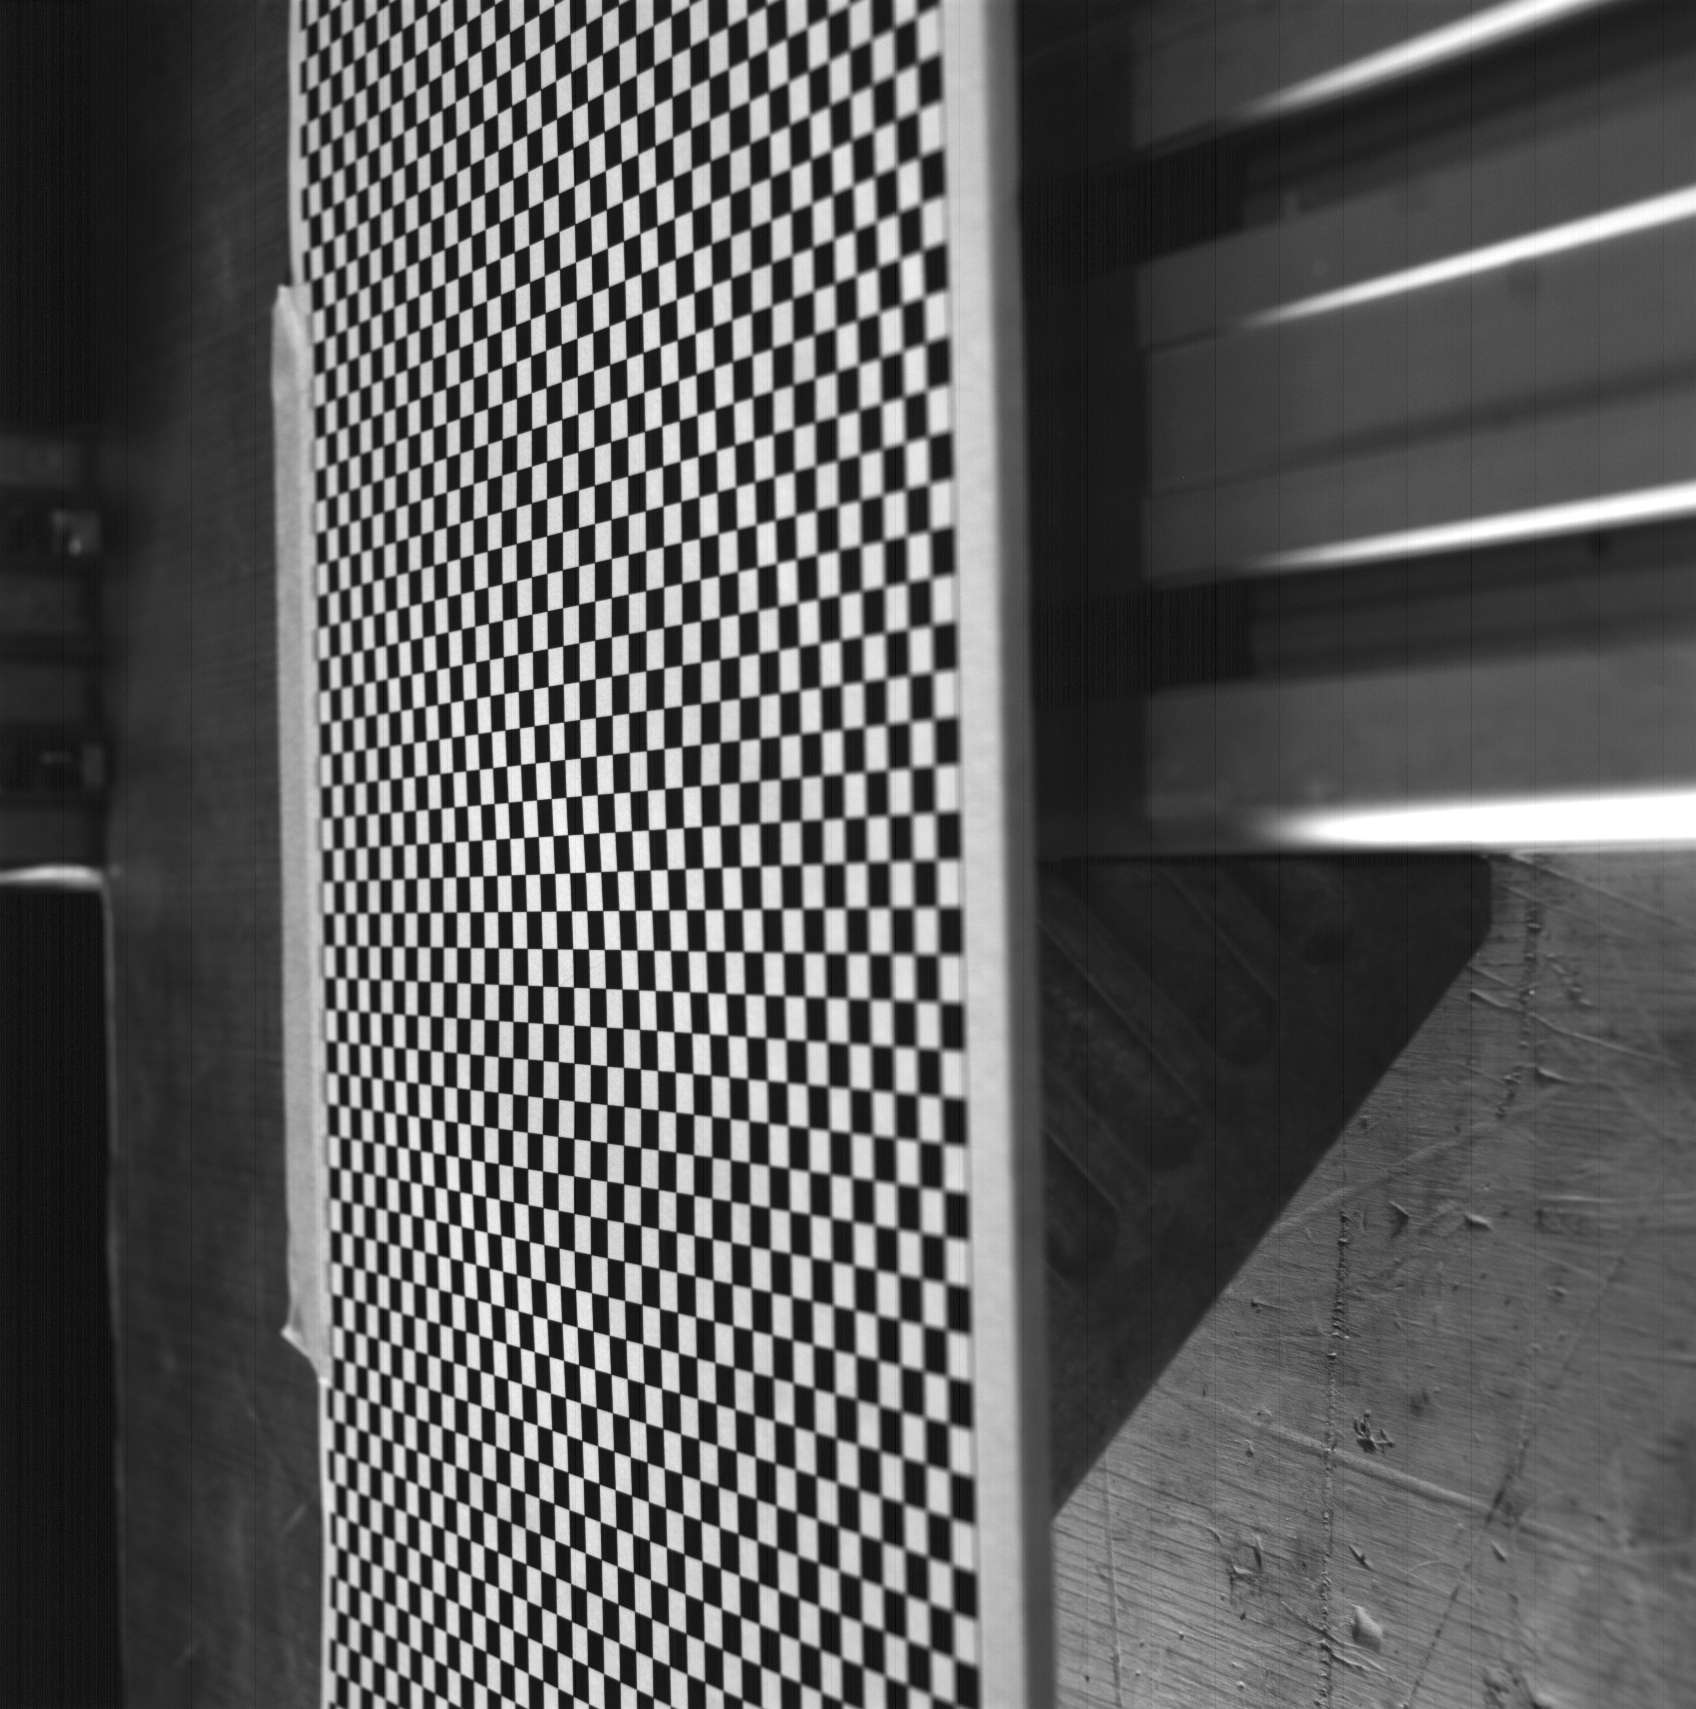
\includegraphics[angle=270, origin=c, width=\textwidth]{./images/analysis/checker09.jpg}
      \caption{Calibration checker with size of squares of $9 \, mm$.}
      \label{fig:calib1}
    \end{minipage}
    \hfill
    \begin{minipage}[c]{.48\textwidth}
      \centering
      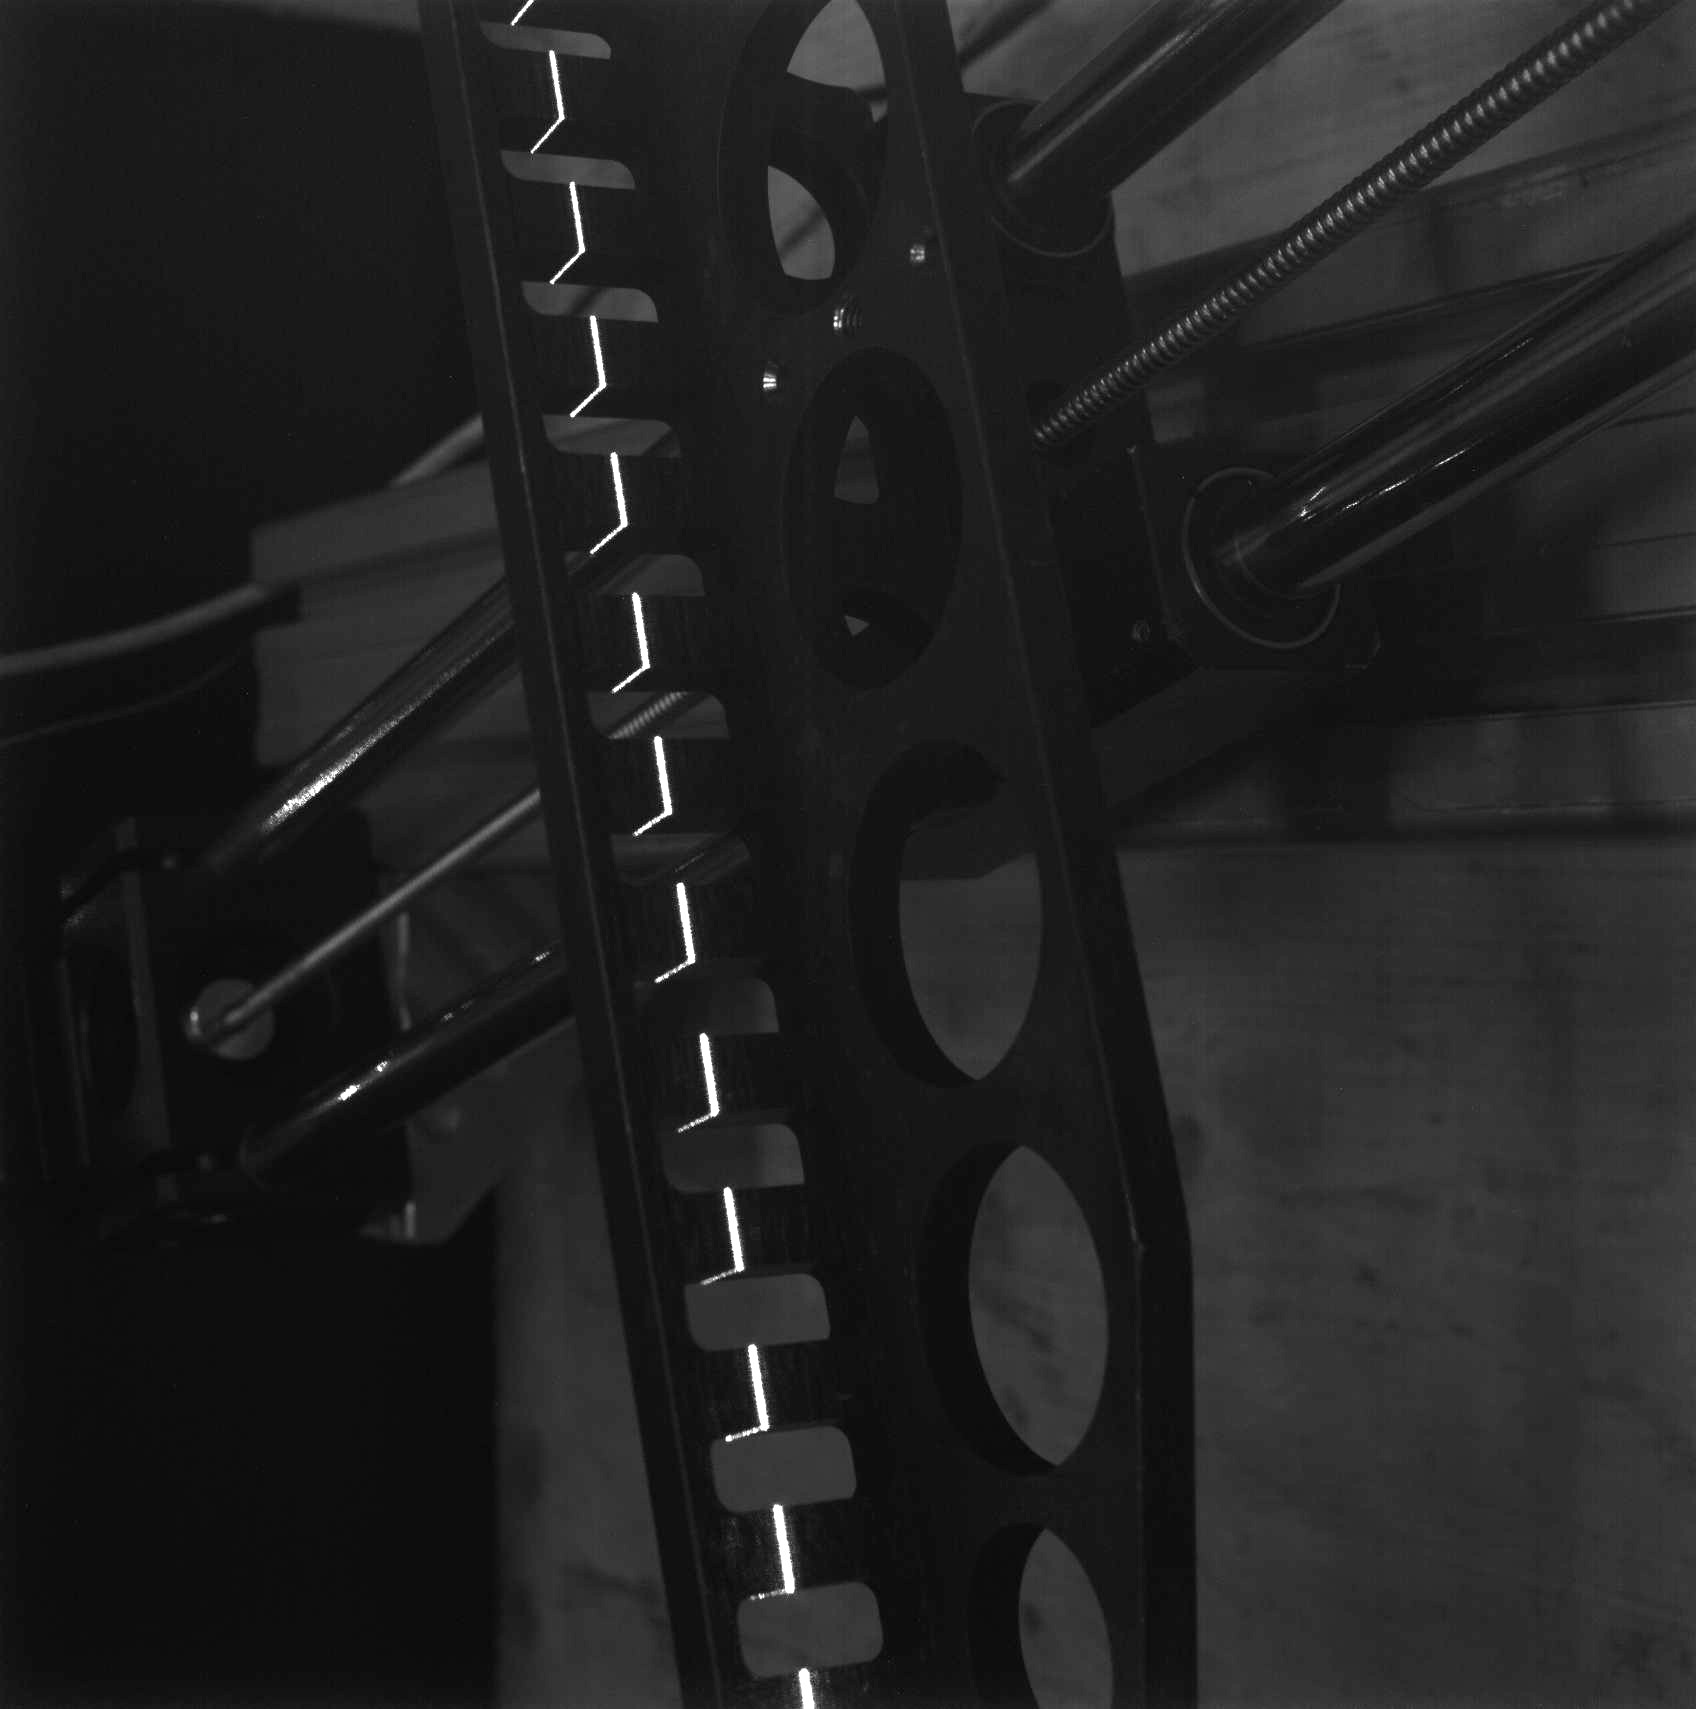
\includegraphics[angle=270, origin=c, width=\textwidth]{./images/analysis/gage.jpg}
      \caption{3D calibration target. \\ ~}
      \label{fig:calib2}
    \end{minipage}
  \end{figure}

  \begin{figure}[t!]
    \begin{minipage}[c]{.48\textwidth}
      \centering
      
\includegraphics[angle=270, origin=c, width=\textwidth]{./images/analysis/laser_profile_over-gage.jpg}
      \caption{Target profile acquired by the camera.}
      \label{fig:calib3}
    \end{minipage}
    \hfill
    \begin{minipage}[c]{.48\textwidth}
      \centering
      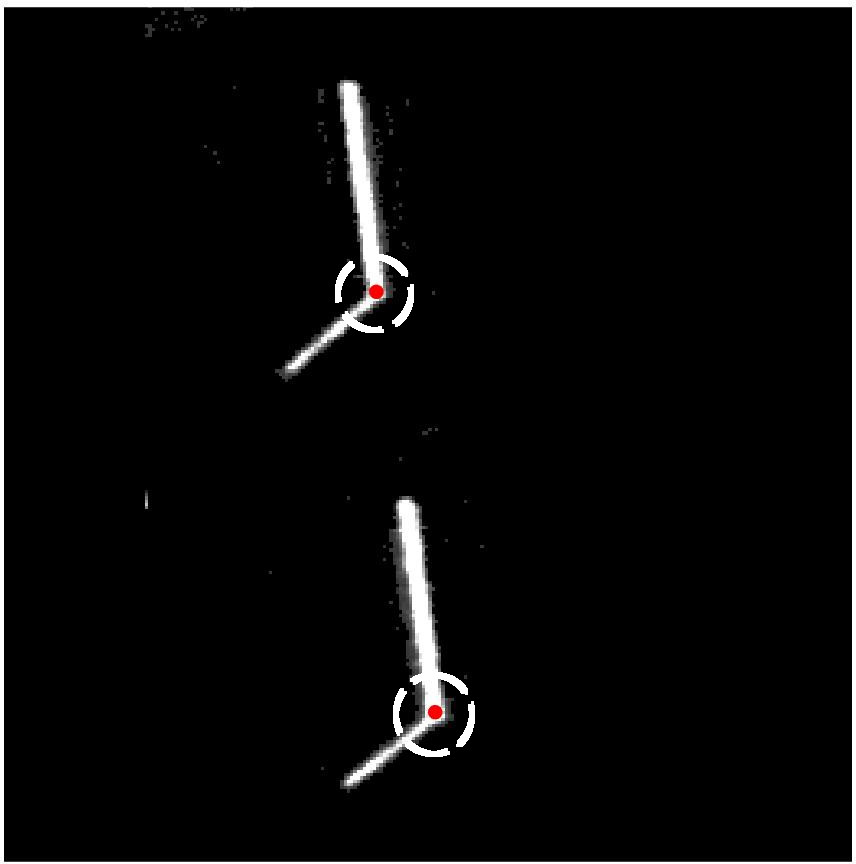
\includegraphics[angle=270, origin=c, width=\textwidth]{./images/analysis/laser_profile_over-gage_corner_det.jpg}
      \caption{Keypoint needed fot the calibration phase.}
      \label{fig:calib4}
    \end{minipage}
  \end{figure}
%    \vfill
%    \begin{minipage}[c]{.48\textwidth}
%      \centering
%      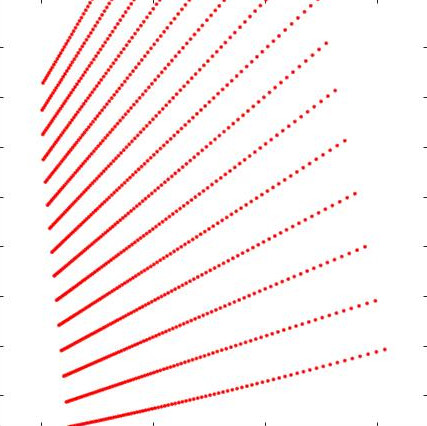
\includegraphics[angle=180, origin=c, width=0.7\textwidth]{./images/analysis/grid.jpg}
%      \caption{Final grid}
%      \label{fig:calib5}
%    \end{minipage}
%    \hfill
%    \begin{minipage}[c]{.48\textwidth}
%      \centering
%      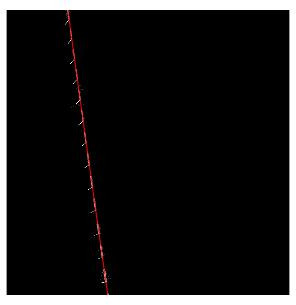
\includegraphics[angle=270, origin=c, width=0.7\textwidth]{./images/analysis/laser_profile_over-gage_fitted.jpg}
%      \caption{Keypoint needed fot the calibration phase.}
%      \label{fig:calib6}
%    \end{minipage}

In the process just described, it is important to consider radial distortion of the lens. What we see in Figure \ref{fig:calib3} is not a straight line, as it is in reality, but because of radial distortion it is a parabola. This mistake leads to the construction of a completely erroneous grid. Another effect of target rotation with respect to the optical axis, is the orientation of the world reference system. This is not a problem, but it is used to apply a correction in order to align the $y$ axis with the \acs{FOV} of the camera, as we assumed in Figure \ref{fig:laser-triang-pdv}. \\

\begin{table}[!t]
  \centering
  \begin{tabular}{@{}cccc@{}}
    \toprule
    \textbf{Measure} & \textbf{Our version}                                                     & \textbf{\textsc{Company version}}                                          & \textbf{Unit}  \\
    \midrule
    $f$ & $36.542$                                                      & $31.971$                                                      & $\left[mm\right]$ \\ && \\
    $k_1$ & $2.24 \cdot 10^{-5}$                                      & $2.3 \cdot 10^{-5}$                                         & $\left[\frac{1}{mm^2}\right]$ \\&& \\
    $T$ & $\begin{bmatrix} 161.605 \\ -35.215 \\ -465.005 \end{bmatrix}$ & $\begin{bmatrix} -157.381 \\ -26.830 \\ 407.198 \end{bmatrix}$ & $\left[mm\right]$ \\&& \\
    $R$ & $\begin{bmatrix}
        -0.770 & -0.638 &  0.015 \\
        -0.415 &  0.482 & -0.772 \\
         0.485 & -0.600 & -0.636 \\
      \end{bmatrix}$ & $\begin{bmatrix}
	     0.765 &  0.644 &  0.009 \\
	     0.480 & -0.562 & -0.673 \\
	    -0.429 &  0.519 & -0.739 \\
      \end{bmatrix}$ & ~ \\ && \\
    $s_x$ & $1$ & $1$ & ~ \\ && \\
    $\left( C_x, C_y \right)$ & $\left(512, 512\right)$                 & $\left(484.387, 918.144\right)$        & $\left[pix\right]$ \\
    \bottomrule
  \end{tabular}
  
  \caption{Comparison between two different version of Tsai's algorithm}
  \label{tab:calib-comparison}
\end{table}
	
In Table \ref{tab:calib-comparison} we compared the results of our implementation of Tsai, with results of a precise implementation, used in industrial systems. The parameters we are interested in are the intrinsic ones. As we can see, the main difference is done by the principal point: in fact, our implementation does not take into account this optimization, so it assumes that the principal point is located in the image center. This is pretty true along the $x$ axis, but not enough along $y$, accordingly with the other version. Furthermore, the difference in focal length is due to the lack of precision of the \textsc{MatLab} optimization functions. \\
As far as extrinsic parameters, however, they depend on the choice of the world reference system that is arbitrarily, thus the sign differences are negligible. From this quick analysis we can concluded not only that our implementation is precise enough for our purposes, but also that the results that we will reach will be a slack lower bounds, that could be improved in real systems implementations. \\

% Fist experiments
  \section{First experiments}
\label{sec:exp1}

In the first set of experiments, we aim to compare our model with the errors made by measuring a well known object, shown in Figure \ref{fig:c5-cad}. The target was made with a \acs{CNC} machine with a precision of $0.1 \, mm$ with respect to all the measures reported in Figure \ref{fig:c5-cad-misure}. Our goal was to reach this measurement precision. \\

The point cloud obtained with our algorithm is shown in Figure \ref{fig:c5-profile_pixel}: the points are plotted in the world reference system, after that we have projected the laser spots, detected in the image.

\begin{figure}
  \begin{minipage}[c]{.44\textwidth}
    \centering
    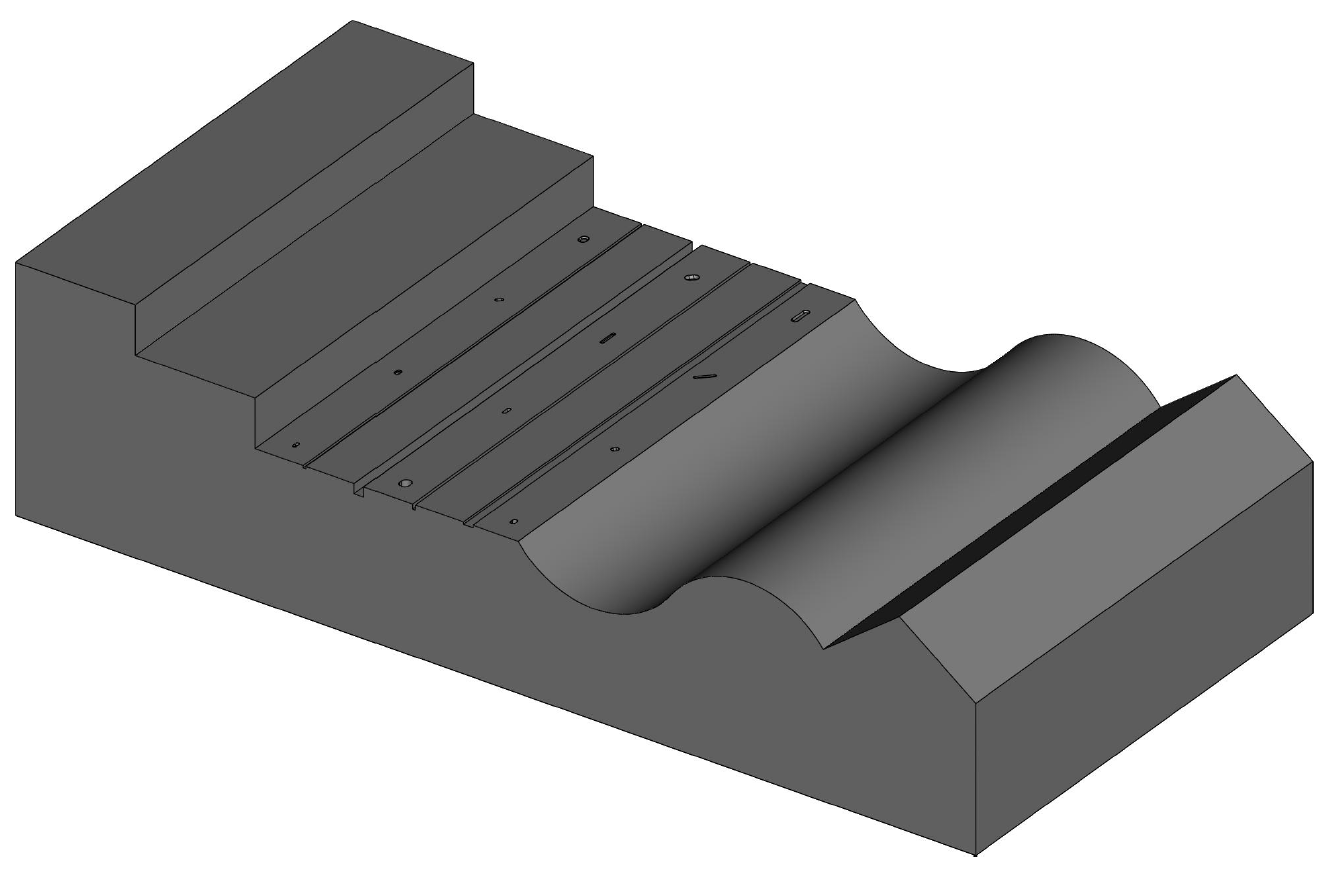
\includegraphics[width=\textwidth]{./images/analysis/t1/cad.png}
    \caption{CAD of the target \\ object}
    \label{fig:c5-cad}
  \end{minipage}
  \hfill
  \begin{minipage}[c]{.55\textwidth}
    \centering
    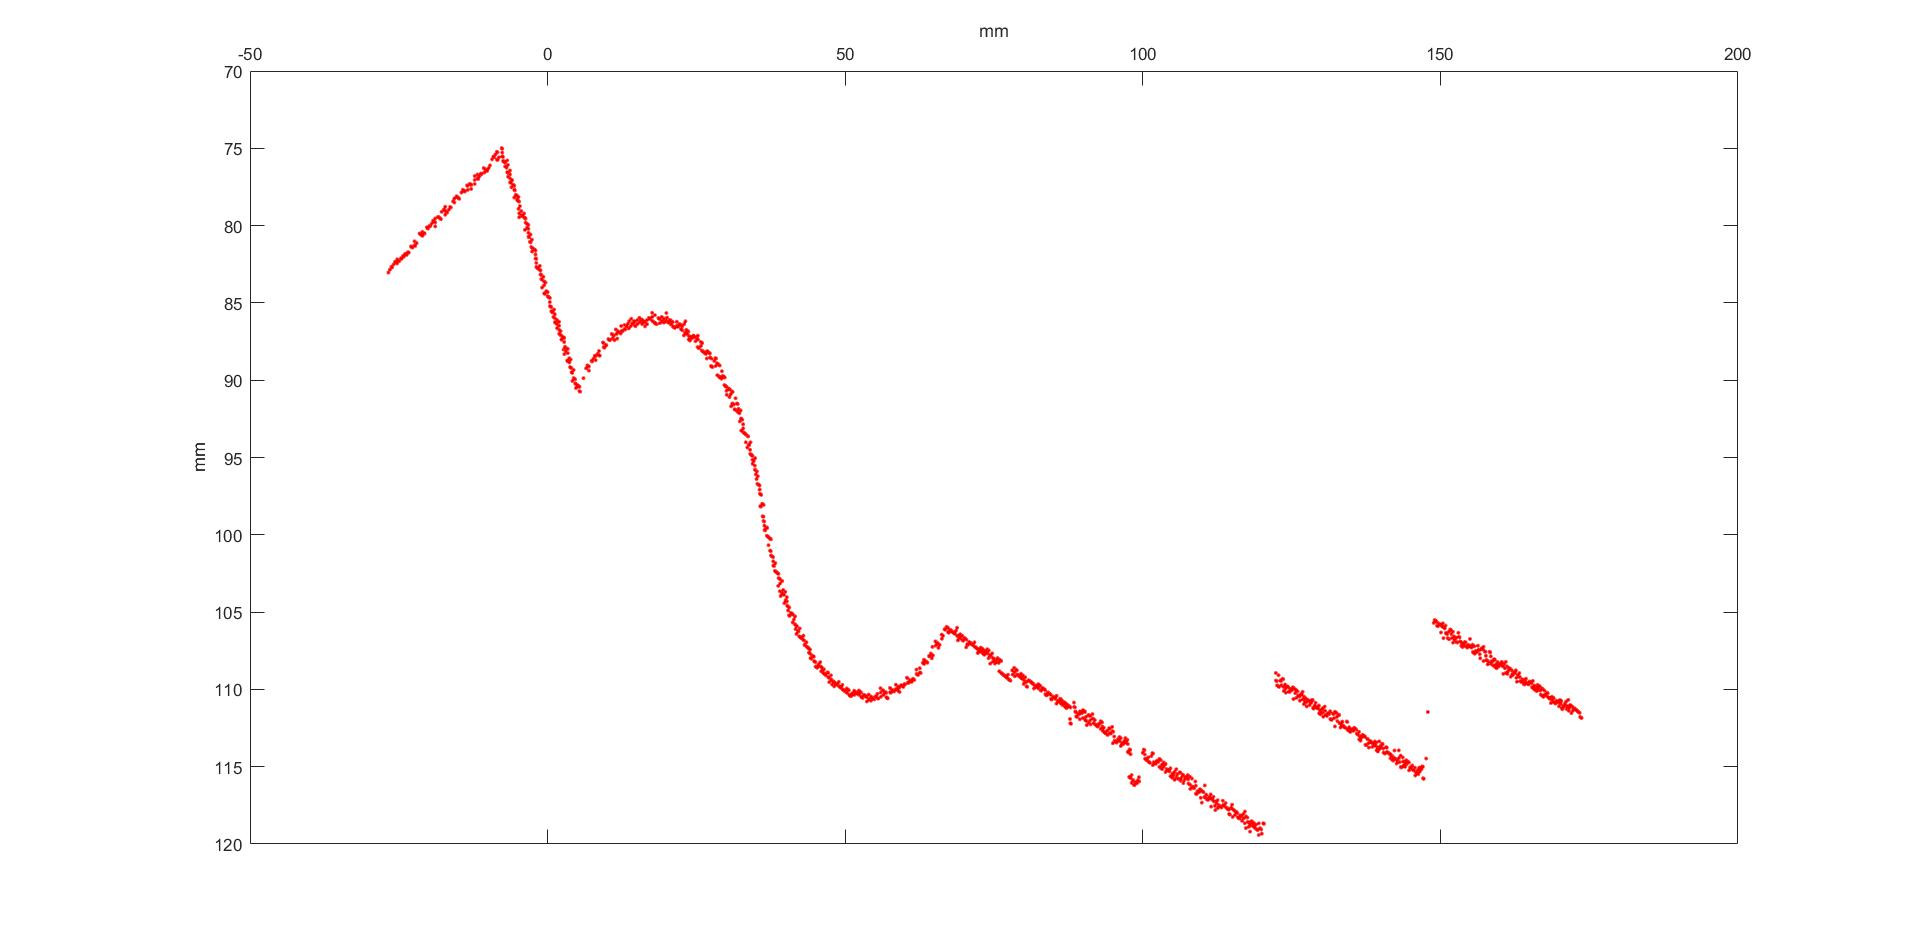
\includegraphics[width=\textwidth]{./images/analysis/t1/pixel_profile_cut.jpg}
    \caption{Laser spots, complete profile}
    \label{fig:c5-profile_pixel}
  \end{minipage}
\end{figure}
\vfill
\begin{figure}
  \centering
  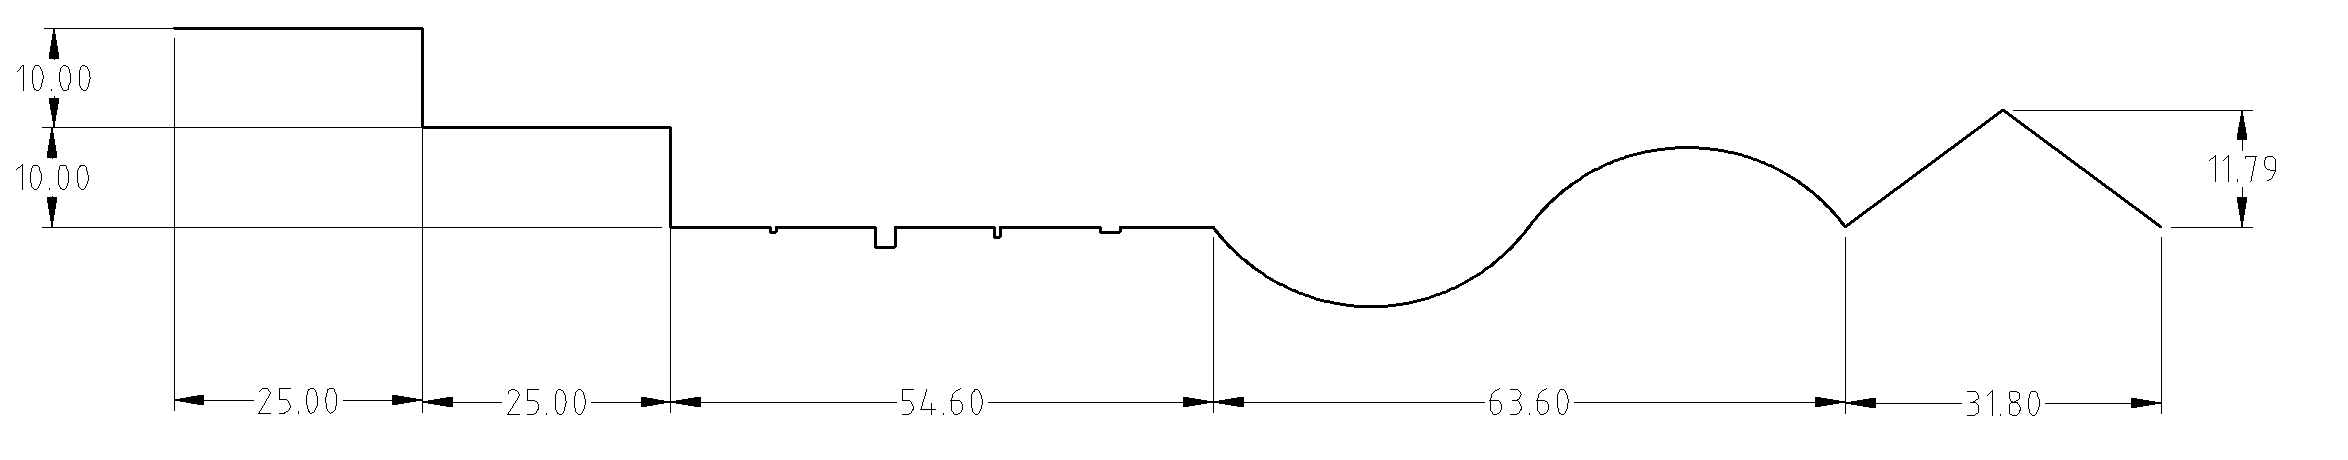
\includegraphics[width=\textwidth]{./images/analysis/t1/cad_misure.png}
  \caption{Measures of the target object}
  \label{fig:c5-cad-misure}
\end{figure}
\vfill
\begin{figure}
  \centering
  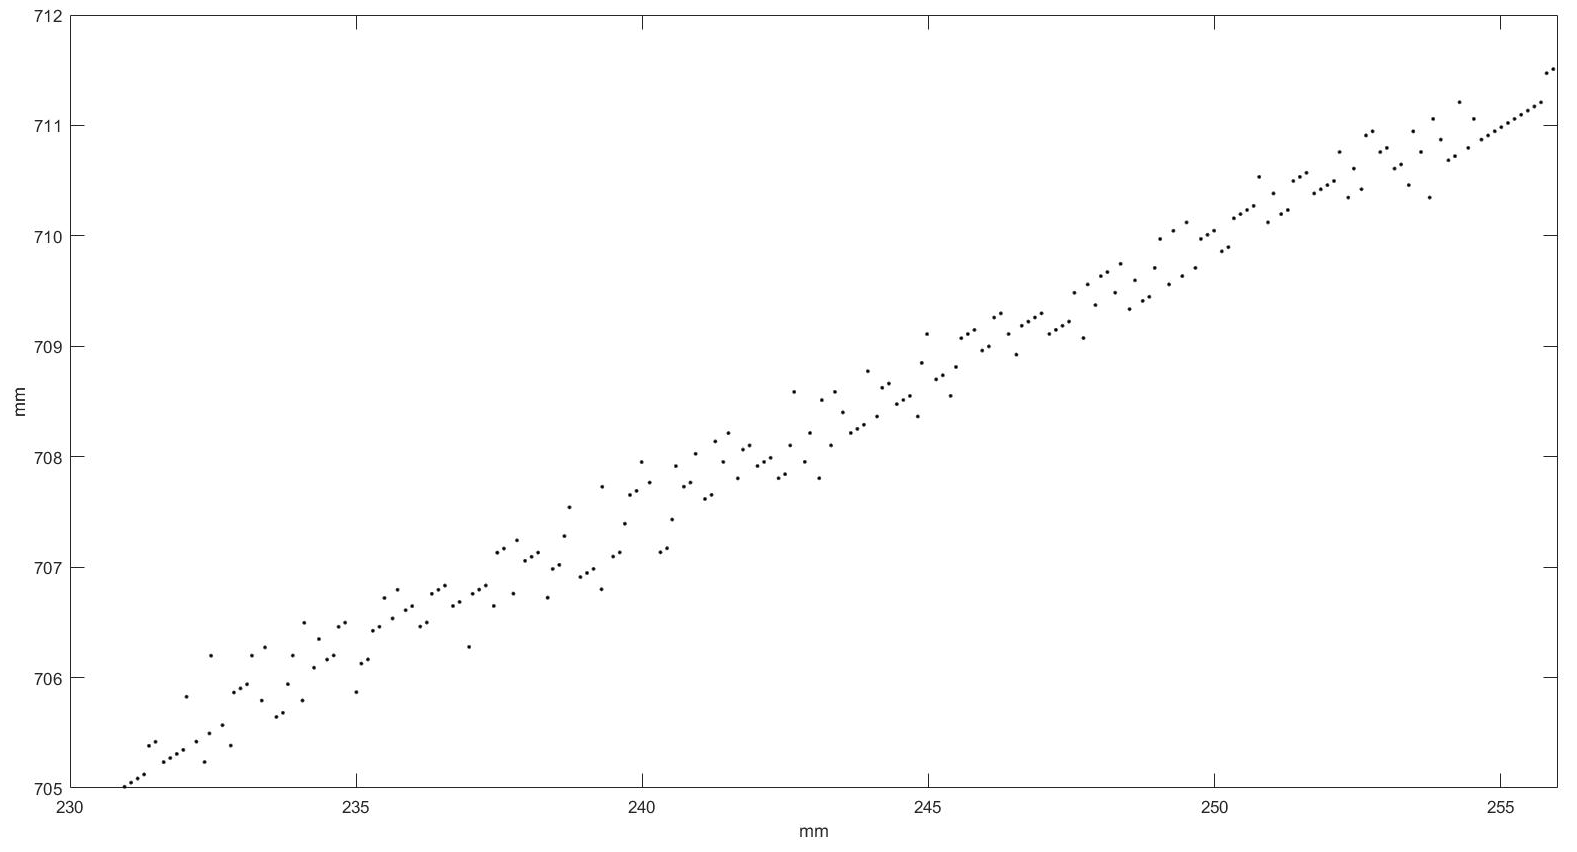
\includegraphics[width=\textwidth]{./images/analysis/t1/pixel_profile_det.jpg}
  \caption{Details of the laser spots}
  \label{fig:c5-profile_pixel_det}
\end{figure}
\vfill
\begin{figure}
  \centering
  \includegraphics[width=\textwidth]{./images/analysis/t1/peak_distrib.jpg}
  \caption{Distribution of the energy along a row of the image. Vertical lines indicate the 3 windows used.}
  \label{fig:c5-peak_distrib}
\end{figure}
\vfill
\begin{figure}
  \centering
  \includegraphics[width=\textwidth]{./images/analysis/t1/com6_cmp.jpg}
  \caption{Comparison of \textit{Center of Mass} applied with extended widow sizes}
  \label{fig:c5-com_cmp_6}
\end{figure}
\vfill
\begin{figure}
  \centering
  \includegraphics[width=\textwidth]{./images/analysis/t1/br6_cmp.jpg}
  \caption{Comparison of \textit{Blais and Rioux} applied with extended widow sizes}
  \label{fig:c5-br_cmp_6}
\end{figure}
\begin{figure}
  \centering
  \includegraphics[width=\textwidth]{./images/analysis/t1/fir6_cmp.jpg}
  \caption{Comparison of \textit{FIR} applied with extended widow sizes}
  \label{fig:c5-fir_cmp_6}
\end{figure}
\clearpage

If we magnify the data, as shown in Figure \ref{fig:c5-profile_pixel_det}, we can observe that the acquired profile is very thick. This effect is due to the noise of the laser beam (e.g. speckle), that causes small variations of the positions of the peaks, along a line of the image. Thus, we expected that the use of sub-pixel filters, should reduce the thickness of the beam. All the model described in Section \ref{sec:laser-peaks}, were introduced considering only few pixel around the candidate to be the peak. So we tried to apply them, using windows of $3$, $5$ and $7$ pixel were possible. \\

Unfortunately, the results made us wrong. Observing the live images, we noticed that the width of the Gaussian was on average equal to $20$ pixels, as the row shown in Figure \ref{fig:c5-peak_distrib}: the used interval are too small with respect to signal amplitude. Hence, we decided to increase the window to $11$ and $16$ pixels where possible. In Figure \ref{fig:c5-com_cmp_6} we can see the improvement of the detail shown in Figure \ref{fig:c5-profile_pixel_det}, obtained using the \textit{center of mass}. Therefore, we concluded that, in order to get a sufficiently precise smoothing, it is necessary that the window is bigger enough to contain the whole laser spot. To complete our analysis, we tried to further increase the size of the window. This tests did not lead to significant improvements over the windows of $11$ or $16$ pixels. On the contrary in some cases, for example in noisy areas of the images, or because the background noise, the use of a larger window deteriorated the peak recognition. \\
We reached the same results analysing the remaining filters, as shown in Figures \ref{fig:c5-br_cmp_6} and \ref{fig:c5-fir_cmp_6}. From these observations, we concluded that the windows sizes have to be comparable with the Gaussian: if they are too small, the profile will be less precise; if they are too big, we risk to add noise.

Regarding the remaining filters (Gaussian, Linear and Parabolic), we have found some difficulties extending them, in order to increase the number of points involved in: as we have already said, $3$ pixels are too few to obtain a good approximation of the laser beam. However, this operation has proved to be meaningless. The three models are based on weighted linear models, such that they work properly only if three pixel are used. Change these weights, changes the meaning of the model itself. The only one that has been extended (the Parabolic) did not reach the results reached with the \textit{\acs{COM}}, the \textit{Blaise\&Rioux} or with the \textit{FIR} filter. Thus, we decided to ignore them from our analysis.

A second observation in support of this choice is due to the saturation effect. Sometimes could happen that some consecutive pixels have the same (maximum) value, caused by changing in the illumination of the working place, out of focus lenses or lasers, or caused by translucid or labertian surfaces. If we use only $3$ or $4$ pixels, it is impossible for these filters to properly identify the peak the the laser spot. \\
  
At this point, we were able to evaluate some measures. To simplify the task, we decided to consider a few well-recognizable points of the profile, i.e. the points used in Figure \ref{fig:c5-cad-misure} to add quotes. Thus, we used a simple 3D corner detector, and the measures were computed as differences between the points, after the alignment of the detected profile to the model. \\
Before achieving remarkable results, we found some difficulties. The most important, is related to calibration. As we said in Section \ref{sec:teo-calibration}, it is fundamental that the grid of calibration points covers the entire \acs{FOV} of the camera. Despite that, the points have to be always on focus. If for any reasons this condition is not true, some of these points could affect the quality of the calibration itself. Thus, we manually reduced the grid until we reached a tiny type I error. \\

Finally, we had got the first results. In Figure \ref{fig:c5-match} we shown the match computed before estimate the measures, while in Tables \ref{tab:c5-r1-teo} and \ref{tab:c5-r1-real} we reported an example of how we estimated the measurement error (theoretically and with empirical data), in particular these results are obtained using the \textit{center of mass} with a window of $16$ pixels. Note that, in order to evaluate column \textit{point error}, we assumed that the event that a point falls in $p = (x, y)$ can be modelled as the union of two i.i.d. events, followed by:
  \begin{equation}
    \sigma_p = \sqrt{\sigma_x^2 + \sigma_y^2}
    \label{eq:exp:var-prop}
  \end{equation}
  \begin{figure}[t!]
    \centering
    \includegraphics[width=\textwidth]{./images/analysis/t1/example_cut.jpg}
    \caption{Example of match of the profile extracted using \textit{center of mass} with window of $16$ pixel. The model is plotted in blue, while the extracted profile is plotted in red.}
    \label{fig:c5-match}
  \end{figure}
  \begin{table}[b!]
\centering
\begin{tabular}{|r|r|r|r|}
\hline
\multicolumn{1}{|c|}{\textbf{Approximation}} & \multicolumn{1}{c|}{\textbf{Y Error}} & \multicolumn{1}{c|}{\textbf{X Error}} & \multicolumn{1}{c|}{\textbf{Point Error}} \\ \hline
\multicolumn{1}{|c|}{\textit{(pix)}}           & \multicolumn{1}{c|}{\textit{(mm)}}      & \multicolumn{1}{c|}{\textit{(mm)}}      & \multicolumn{1}{c|}{\textit{(mm)}}          \\ \hline
0.1089                                       & 0.0153                                & 0.5678                                & 0.5680                                    \\ \hline
0.1089                                       & 0.0101                                & 0.3261                                & 0.3263                                    \\ \hline
0.1089                                       & 0.0073                                & 0.6246                                & 0.6246                                    \\ \hline
0.1089                                       & 0.0095                                & 0.7877                                & 0.7877                                    \\ \hline
0.1089                                       & 0.0528                                & 0.9875                                & 0.9889                                    \\ \hline
0.1089                                       & 0.0534                                & 0.6900                                & 0.6921                                    \\ \hline
0.1089                                       & 0.1157                                & 0.8070                                & 0.8152                                    \\ \hline
0.1089                                       & 0.1172                                & 0.4760                                & 0.4902                                    \\ \hline
0.1089                                       & 0.2220                                & 0.5741                                & 0.6155                                    \\ \hline
\multicolumn{3}{|r|}{\textbf{Mean}}                                                                                          & \textbf{0.6565}                           \\ \hline
\end{tabular}
\caption{Theoretical results obtained using the \textit{Center of Mass} with window of 16 pixel}
\label{tab:c5-r1-teo}
\end{table}
  \begin{table}[h!]
\centering
\begin{tabular}{|r|r|r|r|r|r|r|}
\hline
\multicolumn{3}{|c|}{\textbf{Abscissa}}                                                                             & \multicolumn{3}{c|}{\textbf{Ordinate}}                                                                             & \multicolumn{1}{c|}{\multirow{2}{*}{\textbf{Point Error}}} \\ \cline{1-6}
\multicolumn{1}{|c|}{\textbf{Model}} & \multicolumn{1}{c|}{\textbf{Profile}} & \multicolumn{1}{c|}{\textbf{Errors}} & \multicolumn{1}{c|}{\textbf{Model}} & \multicolumn{1}{c|}{\textbf{Profile}} & \multicolumn{1}{c|}{\textbf{Errors}} & \multicolumn{1}{c|}{}                                      \\ \hline
\multicolumn{1}{|c|}{\textit{(mm)}}           & \multicolumn{1}{c|}{\textit{(mm)}}      & \multicolumn{1}{c|}{\textit{(mm)}}      & \multicolumn{1}{c|}{\textit{(mm)}} & \multicolumn{1}{c|}{\textit{(mm)}}      & \multicolumn{1}{c|}{\textit{(mm)}}      & \multicolumn{1}{c|}{\textit{(mm)}}          \\ \hline
15.9010                              & 16.5450                               & 0.6438                               & 11.7920                             & 12.2720                               & 0.4804                               & 0.8033                                                     \\ \hline
15.9000                              & 16.5160                               & 0.6157                               & 11.7920                             & 11.8430                               & 0.0511                               & 0.6178                                                     \\ \hline
63.6000                              & 63.1840                               & 0.4159                               & 0.0000                              & 0.0909                                & 0.0909                               & 0.4257                                                     \\ \hline
54.6000                              & 54.4860                               & 0.1144                               & 0.0000                              & 0.0863                                & 0.0863                               & 0.1433                                                     \\ \hline
0.0000                               & 0.2235                                & 0.2235                               & 10.0000                             & 10.4530                               & 0.4530                               & 0.5051                                                     \\ \hline
25.0000                              & 25.6950                               & 0.6949                               & 0.0000                              & 0.5067                                & 0.5067                               & 0.8600                                                     \\ \hline
0.0000                               & 0.7019                                & 0.7019                               & 10.0000                             & 10.2750                               & 0.2746                               & 0.7537                                                     \\ \hline
25.0000                              & 25.4190                               & 0.4189                               & 0.0000                              & 0.1010                                & 0.1010                               & 0.4309                                                     \\ \hline
\multicolumn{6}{|r|}{\textbf{Mean}}                                                                                                                                                                                                      & \textbf{0.5675}                                            \\ \hline
\end{tabular}
\caption{Results obtained using the \textit{Center of Mass} with window of 16 pixel}
\label{tab:c5-r1-real}
\end{table}

In Table \ref{tab:c5-r1-all}, instead, we have summarized the results obtained with all the filters considered. As we can see, they are significantly higher than the $0.1 \, mm$ that we wanted to reach. However, some considerations can already be made.
  \begin{table}[t!]
\centering
\begin{tabular}{|c|c|r|r|r|}
\hline
\textbf{\textbf{Error}}  & \multicolumn{1}{l|}{\textbf{Window}} & \multicolumn{2}{c|}{\textbf{Theoretical}}                                & \multicolumn{1}{c|}{\textbf{Empirical}} \\ \hline
\textit{}                   & \textit{}                            & \multicolumn{1}{c|}{\textit{(pix)}}       & \multicolumn{1}{c|}{\textit{(mm)}}        & \multicolumn{1}{c|}{\textit{(mm)}}      \\ \hline
\textit{\textbf{Pixel}} & 1                                    & 0.2887                                    & 0.6579                                    & 0.6764                                  \\ \hline
\textit{\textbf{COM}}   & 16                                   & 0.1089                                    & 0.6565                                    & 0.5675                                  \\ \hline
\textit{\textbf{COM}}   & 20                                   & 0.0921                                    & 0.6565                                    & 0.5628                                  \\ \hline
\textit{\textbf{BR}}    & 16                                   & 0.1498                                    & 0.6596                                    & 0.5365                                  \\ \hline
\textit{\textbf{BR}}    & 20                                   & 0.1471                                    & 0.6558                                    & 0.3263                                  \\ \hline
\textit{\textbf{FIR}}   & 16                                   & 0.1671                                    & 0.6564                                    & 0.3654                                  \\ \hline
\end{tabular}
\caption{Summary of the results obtained with the filters used.}
\label{tab:c5-r1-all}
\end{table}
  
First of all, it is clear that all the proposed filters increase the precision of the spot localization. Then, it seems that the assumptions made in Section \ref{sec:laser-peaks} about the performances of the filters, are not complete: from a mathematical point of view, the \textit{center of mass} is better; however, in real case, the \textit{Blais\&Rioux} and the \textit{FIR} gave better results.

The second thing to consider, is the quality of the optical bench:
  \begin{itemize}
    \item The laser wasn't good enough, it was too thick and affected by noise. We did several attempts to properly set the properties of the camera, in order to reduce the amount of light collected by the sensor, i.e. reduce the width of the collected laser beam. Nevertheless, the thickness of the resulting profile is about $0.1 \, mm$.
    \item The model wasn't well defined. Many parameters, such as the error of the Scheimpfulg angles, or the error made positioning the laser projector, weren't known.
  \end{itemize}
Regarding this last point, we understood that the parameters not estimated by the model, can be defined in two different ways: on the one hand they strongly depends by the system itself, and by how good it is build; on the other, they allow to evaluate how good it must be made to reach the precision proposed by the model. Thus, in this first experiment, the model was tuned to reach the results empirically obtained, instead that the contrary. \\

All the imprecisions and the found problems, suggested us to use a more precise and well built systems to evaluate the correctness of our model.

% Validation on industrial systems
  \section{Validation on industrial systems}
\label{sec:exp2}
The choice of the new system was a device under development for a \acs{WPMS}, which configuration is reported in Table \ref{tab:conf2}. This new optical bench was more robust than the previous one: the lasers were more thin and less noisy, while all the components are robustly fixed to the box. Nevertheless, it was dial by two different laser-camera pair. As we said in Chapter \ref{ch:sys_cmp}, it is primary to avoid occlusions when we take the profile of a train wheel, because of the presence of the flange. For this reasons, the target used for the second sets of experiments, was a section of a wheel (referred to as \textit{DIMA} in the following), shown in Figure \ref{fig:exp2-dima}. The measures of interests are reported in Table \ref{tab:exp2-measures}, all of them evaluable with a precision of $0.01 \, mm$. The abbreviations used are:
  \begin{itemize}
    \item \textit{FH} - Flange Height
    \item \textit{FT} - Flange Thickness
    \item \textit{QR} - qR quote 
    \item \textit{RW} - Rim Width
    \item \textit{RT} - Rim Thickness
  \end{itemize}

\begin{table}[h!]
  \centering
  \begin{tabular}{ccccc}
  \hline
  \multicolumn{5}{|c|}{\textbf{Camera}}                                                                                                                                                                            \\ \hline
  \multicolumn{1}{|c|}{\textbf{Name}} & \multicolumn{1}{c|}{\textbf{Size}}      & \multicolumn{1}{c|}{\textbf{Pixel size}} & \multicolumn{1}{c|}{\textbf{Lens Manufacturer}} & \multicolumn{1}{c|}{\textbf{Focal}} \\ \hline
  \multicolumn{1}{|l|}{}              & \multicolumn{1}{c|}{\textit{pix x pix}} & \multicolumn{1}{c|}{\textit{$\mu$m}}        & \multicolumn{1}{c|}{}                           & \multicolumn{1}{c|}{\textit{mm}}    \\ \hline
  \multicolumn{1}{|l|}{Arya}          & \multicolumn{1}{c|}{4096 x 3072}        & \multicolumn{1}{c|}{5.5}                 & \multicolumn{1}{c|}{Zeiss}                      & \multicolumn{1}{c|}{50}             \\ \hline
  \multicolumn{1}{l}{}                & \multicolumn{1}{l}{}                    & \multicolumn{1}{l}{}                     & \multicolumn{1}{l}{}                            & \multicolumn{1}{l}{}                \\ \cline{2-4}
  \multicolumn{1}{c|}{}               & \multicolumn{1}{c|}{\textbf{Laser}}     & \multicolumn{1}{c|}{}                    & \multicolumn{1}{c|}{}                           &                                     \\ \cline{2-4}
  \multicolumn{1}{c|}{}               & \multicolumn{1}{c|}{\textbf{Frequency}} & \multicolumn{1}{c|}{\textbf{Power}}      & \multicolumn{1}{c|}{\textbf{Aperture}}          &                                     \\ \cline{2-4}
  \multicolumn{1}{c|}{\textit{}}      & \multicolumn{1}{c|}{\textit{nm}}        & \multicolumn{1}{c|}{\textit{W}}          & \multicolumn{1}{c|}{\textit{degree}}            & \textit{}                           \\ \cline{2-4}
  \multicolumn{1}{c|}{}               & \multicolumn{1}{c|}{450}                & \multicolumn{1}{c|}{3.5}                 & \multicolumn{1}{c|}{45}                         &                                     \\ \cline{2-4}
  \end{tabular}
  
  \caption{Configuration of the second system.}
  \label{tab:conf2}
\end{table}

The first step was to compare the results of our calibration algorithm with the ones of the company. Differently from the previous case, the presence of two laser-camera pair required to calibrate both of them, independently one from the other. After that, a second round of calibration was needed to determine the relations to use to merge the two profiles. Note that this scenario gave us some issue later, in particular because of the two pairs
  \begin{figure}
    \centering
    \includegraphics[width=\textwidth]{./images/analysis/exp2/DIMA.jpg}
    \caption{Photo of the DIMA}
    \label{fig:exp2-dima}
  \end{figure}
\vfill
  \begin{table}
\centering
\begin{tabular}{|c|c|c|c|c|}
\hline
\textbf{FH}   & \textbf{FT}   & \textbf{QR}   & \textbf{RW}   & \textbf{RT}   \\ \hline
\textit{(mm)} & \textit{(mm)} & \textit{(mm)} & \textit{(mm)} & \textit{(mm)} \\ \hline
$28.00$       & $32.52$       & $10.81$       & $135.01$      & $47.11$         \\ \hline
\end{tabular}
\caption{Measures of the DIMA}
\label{tab:exp2-measures}
\end{table}
\vfill
  \begin{figure}
    \centering
    \includegraphics[width=\textwidth]{./images/analysis/exp2/wheel_steps.jpg}
    \caption{Steps used to merged the two profiles}
    \label{fig:exp2-merged}
  \end{figure}
\noindent
which used two different configurations, e.g. in terms of baselines length and triangulation angles. However, once again, all the parameters where comparable between the two algorithms, thus we continued with our analysis.

The second step, was the evaluation of the profile. Using the results of the previous set of experiments, we focused only on the \textit{center of mass}, \textit{Blais\&Rioux} and \textit{FIR} filters, ignoring the others. The windows used where of $16$ and $20$ pixels for each filter. After several attempts we correctly merged the two profiles collected by the two laser-camera pairs. To do that, we first converted the filtered laser in the world reference system, than we superimposed the two profiles and merged them in the same data structure. At the end we smoothed a bit the obtained profile, in order to reduce the effect of noise and the laser thickness, especially along the inner ad outer sides. The result reached is shown in Figure \ref{fig:exp2-merged}. \\

As shown in the last sub-plot, we had to pay attention when using \textsc{MatLab} functions: to increase the precision of this process, we decided to split the wheel's section in many parts, using the keypoints described above as extreme points of these curves; thus, we used a different mathematical model to smooth each part. During this process, it could happen that some gaps appear in the smoothed profile, reducing the precision of points location. As we will see, we can consider these errors negligible in our working conditions. \\

Finally, numerical results are shown. In Table \ref{tab:exp2:refereces} we reported an approximation of the errors committed at the center of the \acs{FOV}. It is already possible to see that, despite the improving given by the filters at pixel level, we haven't a same increase on the world reference system, i.e. in $mm$. Carefully analysing each step of the model, we noticed that the performance decreased on Equation \ref{eq:model:err:disc} and on Equation \ref{eq:det_a}. In the first case it is simple to understand why: the multiplication by the pixel size considerably reduces the weight of the error, especially if the pixel size is in the order of tenths of a millimiter. To be precise, this is not an error reduction, rather a change of scale, from pixel to millimeters; the smaller the pixel is, the smaller is the weight of the error. Regarding the second case, instead, we didn't find a good answer that can explain what happened. From our point of view, we could interpret this situation as an another change of reference system, from the camera to the world. However, the change of unit of measure was performed in case before. The only thing that can help us is that, a variation in the point in the space corresponds to a much smaller variation in the sensor, so the error is more apparent on the latter plane, rather than in the world.
  \begin{table}[h!]
  \centering
  \begin{tabular}{|l|r|r|r|r|}
    \hline
    \multirow{2}{*}{}  & \multicolumn{1}{c|}{\textbf{Approximation}} & \multicolumn{1}{c|}{\textbf{Y}}    & \multicolumn{1}{c|}{\textbf{X}}    & \multicolumn{1}{c|}{\textbf{Point error}} \\
	\hline
                       & \multicolumn{1}{c|}{\textit{(pixel)}}    & \multicolumn{1}{c|}{\textit{(mm)}} & \multicolumn{1}{c|}{\textit{(mm)}} & \multicolumn{1}{c|}{\textit{(mm)}}  \\
	\hline
    \textbf{Pixel}    & 0,4083    & 0,0353    & 0,0199    & 0,0405 \\
    \hline
    \textbf{CoM 16}   & 0,1877    & 0,0322    & 0,0195    & 0,0377 \\
    \hline
    \textbf{CoM 20}   & 0,1062    & 0,0316    & 0,0195    & 0,0372 \\
    \hline
    \textbf{BR 16}    & 0,1413    & 0,0319    & 0,0195    & 0,0374 \\
    \hline
    \textbf{BR 20}    & 0,1302    & 0,0318    & 0,0195    & 0,0373 \\
    \hline
    \textbf{FIR}      & 0,2587    & 0,0330    & 0,0196    & 0,0384 \\
    \hline
  \end{tabular}
  
  \caption{Reference values for propagation of the error (model output at the center of the \acs{FOV})}
  \label{tab:exp2:refereces}
\end{table}

Nevertheless, a comparison from theoretical and real results is shown in Table \ref{tab:exp2:means}. The values are the averages over the five measures mentioned above, evaluated using the points shown in Figure \ref{fig:exp2-cad}. As of the theoretical measures, they are estimated as differences between the values in column \textit{point error} of the Table \ref{tab:exp2:refereces}, but evaluated for the keypoints in figure. As we can see, the model is validated: the variation between theoretical and empirical results is comparable with the theoretical variance, so we can consider the results identical. There are only few consideration to take into account.
  \begin{table}[t!]
  \centering
  \begin{tabular}{|l|rr|rr|}
  \hline
  \multirow{3}{*}{} & \multicolumn{1}{c}{\textbf{\begin{tabular}[c]{@{}c@{}}Theoretical\\ Errors\end{tabular}}} & \multicolumn{1}{c|}{\textbf{Variance}} & \multicolumn{1}{c}{\textbf{\begin{tabular}[c]{@{}c@{}}Empirical\\ Errors\end{tabular}}} & \multicolumn{1}{c|}{\textbf{Variance}} \\
  \hline
  & \multicolumn{1}{c}{\textit{$(\mu m)$}}    & \multicolumn{1}{c|}{\textit{$(\mu m)$}}     & \multicolumn{1}{c}{\textit{$(\mu m)$}}    & \multicolumn{1}{c|}{\textit{$(\mu m)$}}     \\
  \hline
  \textbf{Pixel}     & 36.2    & 0.001400    & 105.1    & 5.9 \\
  \hline
  \textbf{CoM 16}    & 29.6    & 0.000973    & 32.1     & 0.5 \\
  \hline
  \textbf{CoM 20}    & 28.2    & 0.000823    & 33.5     & 0.7 \\
  \hline
  \textbf{BR 16}     & 28.8    & 0.000917    & 32.8     & 0.6 \\
  \hline
  \textbf{BR 20}     & 28.6    & 0.000875    & 30.0     & 0.4 \\
  \hline
  \textbf{FIR}       & 31.4    & 0.001240    & 29.6     & 0.3 \\
  \hline
  \end{tabular}
  
  \caption{Averages of the computed measures}
  \label{tab:exp2:means}
\end{table}

  \begin{figure}[t!]
    \centering
    \includegraphics[width=0.88\textwidth]{./images/analysis/exp2/wheel_profile_mod.jpg}
    \caption{Analysed profile, with measure indication, CAD style.}
    \label{fig:exp2-cad}
  \end{figure}
As we said at the beginning of this section, we are using two laser-camera pairs, which results are merged to obtain the profile. The two systems used different configurations, in particular different triangulation angles and baselines. Despite this, differences are very small in terms of absolute values, we noticed that they lead to different output models, i.e. different error approximations. In Table \ref{tab:exp2:refereces}, as in the other phases of our analysis, the values in columns \textit{Y} and \textit{X} are the means of the two models. In this case we consider the means, instead of the error propagation for the variance in Equation \ref{eq:exp:var-prop}, because we didn't know to which piece of the profile the selected point belongs. Statistically, we had a probability of an half, thus we considered the mean as the most appropriate operator.

Another doubt we still had, regards the tuning of the model. Also in this case, we missed some informations, such as the precision of the Scheimpflug angle, or the orientation of the laser (it is a degree of freedom of the system). Thus, we needed to perform a tuning in order to balance the output with the empirical results. Notwithstanding the values used were reasonable with respect to the system structure, we thought that in this way, we mixed some errors due to the model and to the algorithm used to align and merge the two profiles. \\

To conclude, we can say that the model seems to be correct. This last set of tests allowed to underline the fact that it is a good approximation of the real scenarios, however, it has some degrees of freedom that must be analysed to get reasonable results. Also in this case, we remarked the importance of using windows comparable to the laser width, on the contrary the effects noise present in the acquired frames could be great enough to predominate on the laser. As far as the camera is concerned, we used here a sensor with pixels sizes smaller than the camera used in the previous section. As we can see, reducing pixels size reduces considerably the performances of the sub-pixel filters: this is reasonable if we think that a smaller pixel represents a smaller part of the world. \\
Two more considerations before continuing, concerning the resolution of the camera and the effects of noise in the frame. During our analysis we noticed that the empirical errors we obtained were very similar to the nominal resolution of the camera. This observation suggested us to control if a same thing happened in the previous set of experiments, and we noticed that it was quite true. Looking at the noise, however, we have noticed how to change the preprocessing of the image being analysed, changing the values of the empirical errors. More in-depth analyses are discussed in the sections bellow.
%
% Validation of the model
  \section{Validation of the model}
For the last set of tests, we returned over the initial optical bench. In this case, we wanted to compare the output of the model with the resolution of the camera, in order to understand if the precision of the measures we can make, is inferiorly limited by camera resolution, or if it is influenced also by some other factors. \\
To reach our goal, we decided to modify the bench a bit: we used a less distorted lens (the one used in the Section \ref{sec:exp1} introduced too much tangential distortion), and we changed the laser to a similar one to that used in Section \ref{sec:exp2}, less noisy and thick than the initial one (configuration in Table \ref{tab:conf3}). Thus, we calibrate the system again, using the company's software. At this point, we performed two different test:
 \begin{itemize}
   \item First, we repeated the experiments in Section \ref{sec:exp1}, using the same known target object.
   \item Second, we empirically evaluated the resolution of the camera, and compared the results with both the nominal value of the camera, and the results obtained in the first point.
 \end{itemize}
 \begin{table}
  \centering
  \begin{tabular}{ccccc}
  \hline
  \multicolumn{5}{|c|}{\textbf{Camera}}                                                                                                                                                                            \\ \hline
  \multicolumn{1}{|c|}{\textbf{Name}} & \multicolumn{1}{c|}{\textbf{Size}}      & \multicolumn{1}{c|}{\textbf{Pixel size}} & \multicolumn{1}{c|}{\textbf{Lens Manufacturer}} & \multicolumn{1}{c|}{\textbf{Focal}} \\ \hline
  \multicolumn{1}{|l|}{}              & \multicolumn{1}{c|}{\textit{pix x pix}} & \multicolumn{1}{c|}{\textit{mum}}        & \multicolumn{1}{c|}{}                           & \multicolumn{1}{c|}{\textit{mm}}    \\ \hline
  \multicolumn{1}{|l|}{Arya}          & \multicolumn{1}{c|}{4096 x 3072}        & \multicolumn{1}{c|}{5.5}                 & \multicolumn{1}{c|}{Shneider}                   & \multicolumn{1}{c|}{35}             \\ \hline
  \multicolumn{1}{l}{}                & \multicolumn{1}{l}{}                    & \multicolumn{1}{l}{}                     & \multicolumn{1}{l}{}                            & \multicolumn{1}{l}{}                \\ \cline{2-4}
  \multicolumn{1}{c|}{}               & \multicolumn{1}{c|}{\textbf{Laser}}     & \multicolumn{1}{c|}{}                    & \multicolumn{1}{c|}{}                           &                                     \\ \cline{2-4}
  \multicolumn{1}{c|}{}               & \multicolumn{1}{c|}{\textbf{Frequency}} & \multicolumn{1}{c|}{\textbf{Power}}      & \multicolumn{1}{c|}{\textbf{Aperture}}          &                                     \\ \cline{2-4}
  \multicolumn{1}{c|}{\textit{}}      & \multicolumn{1}{c|}{\textit{nm}}        & \multicolumn{1}{c|}{\textit{W}}          & \multicolumn{1}{c|}{\textit{degree}}            & \textit{}                           \\ \cline{2-4}
  \multicolumn{1}{c|}{}               & \multicolumn{1}{c|}{450}                & \multicolumn{1}{c|}{1.6}                 & \multicolumn{1}{c|}{45}                         &                                     \\ \cline{2-4}
  \end{tabular}

  \caption{Configuration of the third system.}
  \label{tab:conf3}
\end{table}

% --------- %
\subsection{Model validation}
In the first phase, the experiments were performed as described in Section \ref{sec:exp1}, but now we have limited the propagation of the errors to the single points, rather than proceeding with the measurements as before. Thus, we put the target in three know position: at the beginning, in the middle and at the end of the \acs{FOV}. This allowed us to cover the entire \acs{FOV} of the camera. In Table \ref{tab:exp3-res} we reported the obtained results. As before, the values are the means of the propagate error for each point over the same sub-filter. We repeated our analysis twice because, as we can see, in the first test, the target was taken in wrong positions. However, we reported all the results better to find some correlations with the results discussed in the next subsection. \\
  \begin{table}[b!]
\centering
\begin{tabular}{|l|l|r|r|r|l|l|l|l|}
\cline{1-1} \cline{3-5} \cline{7-9}
\multirow{3}{*}{} &  & \multicolumn{3}{c|}{\textbf{Test 1}}                                                                            &  & \multicolumn{3}{c|}{\textbf{Test 2}}                                                                            \\ \cline{3-5} \cline{7-9} 
                  &  & \multicolumn{1}{c|}{\textbf{Begin}} & \multicolumn{1}{c|}{\textbf{Center}} & \multicolumn{1}{c|}{\textbf{End}}  &  & \multicolumn{1}{c|}{\textbf{Begin}} & \multicolumn{1}{c|}{\textbf{Center}} & \multicolumn{1}{c|}{\textbf{End}}  \\ \cline{3-5} \cline{7-9} 
                  &  & \multicolumn{1}{c|}{\textit{(mm)}}  & \multicolumn{1}{c|}{\textit{(mm)}}   & \multicolumn{1}{c|}{\textit{(mm)}} &  & \multicolumn{1}{c|}{\textit{(mm)}}  & \multicolumn{1}{c|}{\textit{(mm)}}   & \multicolumn{1}{c|}{\textit{(mm)}} \\ \cline{1-1} \cline{3-5} \cline{7-9} 
\textbf{COM 16}   &  & 0.4320                              & 0.5635                               & 0.5915                             &  & 0.2997                              & 0.3211                               & 0.4247                             \\ \cline{1-1} \cline{3-5} \cline{7-9} 
\textbf{COM 20}   &  & 0.4322                              & 0.5638                               & 0.5910                             &  & 0.2798                              & 0.3212                               & 0.4247                             \\ \cline{1-1} \cline{3-5} \cline{7-9} 
\textbf{BR 16}    &  & 0.4322                              & 0.5642                               & 0.5917                             &  & 0.2800                              & 0.3216                               & 0.4251                             \\ \cline{1-1} \cline{3-5} \cline{7-9} 
\textbf{BR 20}    &  & 0.4322                              & 0.5644                               & 0.5636                             &  & 0.2800                              & 0.3217                               & 0.4251                             \\ \cline{1-1} \cline{3-5} \cline{7-9} 
\textbf{FIR}      &  & 0.4323                              & 0.5636                               & 0.5920                             &  & 0.2800                              & 0.3215                               & 0.4250                             \\ \cline{1-1} \cline{3-5} \cline{7-9} 
\end{tabular}
\caption{Error propagation to points, at the begin, the middle and the end of the \acs{FOV}}
\label{tab:exp3-res}
\end{table}
For the moment, the only consideration that we can make is the comparison with the results in Section \ref{sec:exp1}: the use of a less distorted lens, and the use of a better laser reduced significantly the theoretical error that we can commit.

% --------- %
\subsection{Camera resolution}
In the second phase, we decided to integrate our library with a method that allowed us to evaluate the resolution of the camera. To do that, we put the step motor, used to calibrate the system, parallel with the optical axis; in this way the reference object (used to create the grid of points required by Tsai) is perpendicular with the camera. In this case we are not interested in determining the edges of the object, but only to acquire a horizontal laser line. So, we saved six frames: two at the beginning of the \acs{FOV}, two in the middle, and two at the end; in each pair of the acquisitions, the laser lines are $5 \, mm$ apart. This value was chosen arbitrarily to appreciate the distance to the naked eye, and to be able to control the displacement between one position and the other with a tape measure. In Figure \ref{fig:line-pos} are shown the three positions of the target, with respect of the \acs{FOV} of the camera.
  \begin{figure}[!b]
    \centering
    \begin{minipage}[c]{.32\textwidth}
      \centering
      \includegraphics[width=\textwidth]{./images/analysis/exp3/250.jpg}
    \end{minipage}
    \hfill
    \begin{minipage}[c]{.32\textwidth}
      \centering
      \includegraphics[width=\textwidth]{./images/analysis/exp3/380.jpg}
    \end{minipage}
    \hfill
    \begin{minipage}[c]{.32\textwidth}
      \centering
      \includegraphics[width=\textwidth]{./images/analysis/exp3/510.jpg}
    \end{minipage}
    
    \caption{Positions of the target along the \acs{FOV} of the camera}
    \label{fig:line-pos}
  \end{figure}
In Table \ref{tab:exp3:res2} we reported our results: the first two columns are, respectively, the distances and the errors between the pairs of laser lines, while the third column contains the resolution of the camera, evaluated in the three position cited above. As we can see, the filters did not change resolutions substantially, so we can conclude that the resolution of our camera was in the range $\left( 0.27, 0.55 \right) \, mm/pix$. \\
  \begin{table}[t!]
  \centering
  \begin{tabular}{|cl|p{2.3cm}|p{2.3cm}|p{2.3cm}|}
  \hline
  \multicolumn{2}{|c|}{\multirow{2}{*}{}}              & \multicolumn{1}{c|}{\textbf{Mean}} & \multicolumn{1}{c|}{\textbf{Error}} & \multicolumn{1}{c|}{\textbf{Resolution}} \\
  \multicolumn{2}{|c|}{}                               & \multicolumn{1}{c|}{\textit{(mm)}} & \multicolumn{1}{c|}{\textit{(mm)}}  & \multicolumn{1}{c|}{\textit{(mm / pix)}} \\
  \hline
  \multirow{5}{*}{\textbf{Begin}}  & \textit{CoM 16} & 5,3318                            & 0,3318                             & 0,2730                                  \\
                                 & \textit{CoM 20} & 5,3333                            & 0,3333                             & 0,2731                                  \\
                                 & \textit{BR 16}  & 5,2878                            & 0,2878                             & 0,2730                                  \\
                                 & \textit{BR 20}  & 5,3176                            & 0,3176                             & 0,2731                                  \\
                                 & \textit{FIR}    & 5,3565                            & 0,3566                             & 0,2728                                  \\
  \hline
\multirow{5}{*}{\textbf{Center}} & \textit{CoM 16} & 5,6046                            & 0,6046                             & 0,4021                                  \\
                                 & \textit{CoM 20} & 5,5711                            & 0,5711                             & 0,4016                                  \\
                                 & \textit{BR 16}  & 5,7247                            & 0,7247                             & 0,4026                                  \\
                                 & \textit{BR 20}  & 5,6324                            & 0,6324                             & 0,4026                                  \\
                                 & \textit{FIR}    & 5,6177                            & 0,6177                             & 0,4028                                  \\
  \hline
\multirow{5}{*}{\textbf{End}}    & \textit{CoM 16} & 5,7494                            & 0,7494                             & 0,5500                                  \\
                                 & \textit{CoM 20} & 5,7647                            & 0,7647                             & 0,5501                                  \\
                                 & \textit{BR 16}  & 5,9726                            & 0,9726                             & 0,5504                                  \\
                                 & \textit{BR 20}  & 5,7809                            & 0,7809                             & 0,5510                                  \\
                                 & \textit{FIR}    & 6,3786                            & 1,3786                             & 0,5503                                 \\
    \hline
\end{tabular}
\caption{Camera resolution in \textit{mm/pix}, varying sub-pixel filter and location in the \acs{FOV}}
\label{tab:exp3:res2}
\end{table}

If we compare the values in Table \ref{tab:exp3-res} with the ones in Table \ref{tab:exp3:res2}, it is clear that the target wasn't acquired in the same positions, but despite that, we can say that the values are the same. From our point of view, this was an interesting result: if on the one hand, it has further validated the model, determining a physical lower bound that we have reached, on the other it confirmed what we said in Section \ref{sec:exp2} about the ``sensitive points'' of the model. In our case, the performances of the hardware were good enough to make the software's effects on the final results negligible. As we have already said, the smaller the pixel size is, the smaller the gain done by the filters.

% Noise effects
  \section{Noise effects}
To conclude our analysis, in the end we studied the behaviours of the sub-pixel filters varying the noise in the image. As we mentioned in Section \ref{sec:laser-peaks}, the presence of electrical noise in the frames \cite{1334612}, can affect heavily the quality of the peak detection, thus it is a good practice to apply some filters that reduce the weight of this noise during the laser location phase \cite{Naidu1991}. For example, industry experts know that such operations are necessary if you use the \textit{center of mass}: the presence of spikes influences the evaluation of the weighted average. An example of this, is shown in Figure \ref{fig:noise-es}. \\
  \begin{figure}[t!]
    \centering
    \includegraphics[width=\textwidth]{./images/analysis/noise/electrical.jpg}
    \caption{Effects of noise in peak detection. On the left there is a noise free Gaussian, and the \acs{COM} correctly detect the peak. On the right, the noise moves the location (-.) with respect to the correct one (- -).}
    \label{fig:noise-es}
  \end{figure}
  
As far as we are concerned, we have noticed these problems during the test shown in Section \ref{sec:exp2}. Before reaching the discussed results, we tried to apply different image preprocessing algorithms to increase the precision of the peak localizion. So we saw that when we changed the preprocessing, the final results changed too. In Figure \ref{fig:prep-dima} we reported the model trends for each sub-pixel filter used, varying the image preprocessing algorithms. As we can see, not all algorithms improve the results, on the contrary, sometimes they get worse the final error. In addition, we can see that the trend is different between mobile average and derivatives filters. These observations suggested us that not all filters have the same behaviour. Anyway, these results were obtained from a single system, thus we decided to perform some theoretical tests, in order to control the sources of noise. \\

In the second set of tests, we introduced some noise to the Gaussian, varying its \acs{SNR}. In this way we were able to see how much strong are the sub-pixel algorithms with respect to the noise, and thus to the variations in image conditions. To do that, we varied the \acs{SNR} in the range $\left( 0, 30 \right)$ with step $1$, and repeated the test five times per \acs{SNR} step. The averages of the results are shown in Figures \ref{fig:prep1} and \ref{fig:prep2}. We had to split the trends in two graphics to see better what happens. 

The first thing that caught our attention was the fact that, for high values of \acs{SNR}, the initial hypothesis that $\hat{\delta} \in \left( -\frac{1}{2}, \frac{1}{2} \right)$ with respect to the pixel, is false. The only model that always guarantees the hypothesis, is the \textit{FIR}. Unfortunately, we are not able to model this result mathematically. As we said in the previous chapters, the algorithm used to detects the peak, finds the pixel with the greater value along a row, and then applies on it the sub-pixel filters. If we think of a moment, this is a reasonable hypothesis: so we considered the possibility to go out from the pixel as an error due to the noise in the image.

The second important thing to underline, is the effect of the size of the window. As we have said several times, the window has to be comparable with the width of the Gaussian, however, in presence of noise, the bigger the window is, the bigger is the weight of the noise in the measure. We can see this for both \textit{center of mass} and \textit{B\&R}. Furthermore, in the same point we can notice that the \textit{FIR} filter, that is more robust than the others in presence of noise, becomes the worst. \\

Thus, we can conclude that, from a global point of view, the \textit{FIR} filter is the more robust in presence of noise, and it is the more stable, because of its small variance along noise variation. However, for low noise images \textit{center of mass} and \textit{B\&R} models, allow to reach better results. The \textit{B\&R} is the less stable filter, but as shown in Figure \ref{fig:prep-dima}, it is the less sensible (with the \textit{FIR} filter) to image preprocessing. Finally, as far as the window size is concerned, the rule on Gaussian dimension continues to apply. So, there isn't a filter better than the others: their behaviours strictly depends from the scenario we are working on, and from the preprocess applied to the image. Since these considerations are empirical, we suggest to perform some tests in real conditions before choosing what algorithm use in your application.
  \begin{figure}[b!]
    \centering
    \includegraphics[width=0.95\textwidth]{./images/analysis/noise/preprocessing_dima.png}
    \caption{Variation in the model output changing the image preprocessing.}
    \label{fig:prep-dima}
  \end{figure}
\vfill
  \begin{figure}
    \centering
    \includegraphics[width=\textwidth]{./images/analysis/noise/prep1.png}
    \caption{Filters' trends for \acs{SNR} in range $\left( 0, 10 \right)$}
    \label{fig:prep1}
  \end{figure}
\vfill
  \begin{figure}[t!]
    \centering
    \includegraphics[width=\textwidth]{./images/analysis/noise/prep2.png}
    \caption{Filters' trends for \acs{SNR} in range $\left( 10, 30 \right)$}
    \label{fig:prep2}
  \end{figure}
  

%\textbf{COSE CHE HO VOLUTAMENTE LASCIATO INDIETRO}
%\begin{itemize}
%  \item Test sulla lente, che ha dimostrato che aveva qualche problema, perché il calibro mi veniva sinusoidale anziché parabolico
%\end{itemize}
	% Chapter 4
  \chapter{Diameter error propagation model}
\label{ch::diameter}

\textit{In this last chapter we will briefly discuss the error propagation while diameter is estimated. We will present one of the models introduced in Section \ref{sec:sys-cmp} and we will show some experimental results about it.}

% The Erone's model
  \chapter{Description of the complete mathematical model}
\label{ap:model}
\textit{In this appendix we will analyse formally the proposed model, presented in Chapter \ref{ch::model}. Functions derivatives are trivial, so they will not be indicated except where otherwise indicated.}

%--------------------------------------------%
%--------------------------------------------%
\section*{Error propagation along the y axis}
Accordingly with the geometric model for \acs{SOL} systems, we can write:
  \begin{equation}
    \label{app:eq:triangulation}
	y(\alpha) = y_f + z_f \tan(\phi + \alpha)
  \end{equation}
where $y(\alpha)$ is the point $y$ coordinate; $(x_f, y_f, z_f)$ are the principal point projection coordinates in the laser plane (both in the world reference system); $\phi$ is the triangulation angle and $\alpha$ is the angle offset along $y$ axis.
Using the error propagation model for general non-trivial functions, the error is evaluated as follows:
  \begin{equation*}
    \sigma_{y_\alpha} = \sqrt{
      \left( \frac{\partial y}{\partial y_f} \right)^2 \sigma_{y_f}^2
      + \left( \frac{\partial y}{\partial z_f} \right)^2 \sigma_{z_f}^2
      + \left( \frac{\partial y}{\partial \phi} \right)^2 \sigma_\phi^2
      + \left( \frac{\partial y}{\partial \alpha} \right)^2 \sigma_\alpha^2
    }
  \end{equation*} \\

If laser plane doesn't lie on the target section plane, a common practise is applied the so called ``\textit{radial compensation}'' to \ref{app:eq:triangulation} output:
  \begin{equation*}
    y_w = y(\alpha) \cdot cos(\rho)
  \end{equation*}
where $\rho$ is the angle between laser plane and object plane of symmetry.
In this case the final error is:
  \begin{equation}
    \sigma_{y_w} = \sqrt{
      \left( \frac{\partial y_w}{\partial y(\alpha)} \right)^2 \sigma_{y_\alpha}^2
      + \left( \frac{\partial y_w}{\partial \rho} \right)^2 \sigma_\rho^2
    }
    \label{app:eq:sigma-yw}
  \end{equation} \\

A variation of $y_w$ in the world corresponds to a variation of $y_{s_i}$ in the image plane with an angle $\alpha_i$ according to the relation:
  \begin{equation}
    \label{app:eq:triang_angle}
  	\alpha_i = \arctan\left( \frac{y_{s_i}}{f} \right)
  \end{equation}
where $y_{s_i}$ is the point coordinate in the tilted image plane, and $f$ is the focal length. The error propagation is computed as:
  \begin{equation}
  	\sigma_{\alpha_i} = \sqrt{
  	  \left( \frac{\partial \alpha_i}{\partial y_{s_i}} \right)^2 \sigma_{y_{s_i}}^2
  	  + \left( \frac{\partial \alpha_i}{\partial f} \right)^2 \sigma_f^2
  	}
    \label{app:eq:sigma-alpha}
  \end{equation} \\

As it is known, Scheimpflug principle causes tilting of the image plane. Accordingly with \cite{SchCameraCalib}, the relation between tilted coordinates and parallel coordinates to the sensor is given by:
  \begin{equation}
    \label{app:eq:sch_y}
    y_{s_i} = \lambda_1 \frac{y_{p_i}}{\cos\upsilon} =
    \frac{f}{f - x_{p_i}\tan\chi - y_{p_i}\frac{\tan\upsilon}{\cos\chi}} \frac{y_{p_i}}{ \cos\upsilon}
  \end{equation}
where $\upsilon$ is the tilt angle with respect to $y$ axis, and $\chi$ is the swing angle with respect to $x$ axis, either in the image plane coordinates system, parallel to the camera sensor. The constant $\lambda_1$ is function of $f$, $\upsilon$ and $\chi$, and of point coordinates in the last image plane $\left( x_p, y_p \right)$. The error propagation follows:
  \begin{equation*}
    \sigma_{y_{s_i}} = \sqrt{
      \left( \frac{\partial y_{s_i}}{\partial y_{p_i}} \right)^2 \sigma_{y_{p_i}}^2 +
      \left( \frac{\partial y_{s_i}}{\partial x_{p_i}} \right)^2 \sigma_{x_{p_i}}^2 +
      \left( \frac{\partial y_{s_i}}{\partial \upsilon} \right)^2 \sigma_\upsilon^2 +
      \left( \frac{\partial y_{s_i}}{\partial \chi} \right)^2 \sigma_\chi^2 +
      \left( \frac{\partial y_{s_i}}{\partial f} \right)^2 \sigma_f^2
    }
  \end{equation*}
In this case we indicate the partial derivatives for completeness: \\
\begin{equation*}
  \begin{array}{rl}
    \frac{
      \partial y_s}{\partial y_p} = &
          \frac{f\cdot\sec\upsilon}{f -y_p\cdot\sec\chi\tan\upsilon - x_p\cdot\tan\chi} +
          \frac{f\cdot y_p\cdot \sec\chi\tan\upsilon\sec\upsilon}{\left( f -y_p\cdot\sec\chi\tan\upsilon - x_p\cdot\tan\chi \right)^2} \\~\\
      \frac{\partial y_s}{\partial x_p} = &
          \frac{f\cdot y_p\cdot \tan\chi\sec\upsilon}{\left( f -y_p\cdot\sec\chi\tan\upsilon - x_p\cdot\tan\chi \right)^2} \\~\\
      \frac{\partial y_s}{\partial \chi} = &
          \frac{f\cdot y_p\cdot \sec\upsilon \left( -y_p\cdot \tan\chi\sec\chi\tan\upsilon - x_p\cdot\sec^2\chi \right)}{\left( f -y_p\cdot\sec\chi\tan\upsilon - x_p\cdot\tan\chi \right)^2} \\~\\
      \frac{\partial y_s}{\partial \upsilon} = &
          \frac{f\cdot y_p^2\cdot \sec\chi\sec^3\upsilon}{ \left( f -y_p\cdot\sec\chi\tan\upsilon - x_p\cdot\tan\chi \right)^2} +
          \frac{f\cdot y_p\cdot \sec\upsilon\tan\upsilon}{f -y_p\cdot\sec\chi\tan\upsilon - x_p\cdot\tan\chi} \\~\\
      \frac{\partial y_s}{\partial f} = &
          \frac{f\cdot y_p\cdot \sec\upsilon}{ \left( f -y_p\cdot\sec\chi\tan\upsilon - x_p\cdot\tan\chi \right)^2} +
          \frac{y_p\cdot \sec\upsilon}{f -y_p\cdot\sec\chi\tan\upsilon - x_p\cdot\tan\chi}
  \end{array}
\end{equation*} \\

Developing this model, we took into account only the first order lens radial distortion:
  \begin{equation}
  	\label{app:eq:sensor_to_camera_distortion}
    \begin{matrix}
      y_{p_i} = y_{p_i}^{d} \left( 1 + k_1r^2 \right) \\~\\
      \sigma_{y_{p_i}} = \sqrt{
        \left( \frac{\partial y_{p_i}}{\partial y_{p_i}^d} \right)^2 \sigma_{y_{p_i}^d}^2
        + \left( \frac{\partial y_{p_i}}{\partial k_1} \right)^2 \sigma_{k_1}^2
      }
    \end{matrix}
  \end{equation}
Where $y_{p_i}^d$ is the distorted coordinate in the sensor plane, $k_1$ is the lens radial distortion first order coefficient and $r$ is the lens radius, estimated in the worst case as $r = \frac{image \, size}{2}$. \\

The distorted coordinate in sensor plane is evaluate accordingly with:
  \begin{equation}
      \label{app:eq:sensor_to_camera_center}
      y_{p_i}^d = d'_y (y_{c_i} - c_y)
  \end{equation}
where $c_y$ is the $y$ coordinate of the center image, $d'_y$ is the normalized center to center distance between adjacent sensor elements, and $y_c$ is the point coordinate in pixel. Its error is computed as:
  \begin{equation*}
    \sigma_{y_{p_i}^d} = \sqrt{
      \left( \frac{\partial y_{p_i}^d}{\partial y_{c_i}} \right)^2 \sigma_{y_{c_i}}^2
      + \left( \frac{\partial y_{p_i}^d}{\partial c_y} \right)^2 \sigma_{c_y}^2
    }
  \end{equation*} \\

At the end of the chain, the sub-pixel approximation error is evaluated as follows:
  \begin{equation*}
    \sigma_{y_{c_i}} = |\delta_i - \hat{\delta}_i|
  \end{equation*}
where $\delta_i$ is the real laser peak position inside the pixel, and $\hat{\delta}_i$ is the approximated peak position.

%--------------------------------------------%
%--------------------------------------------%
\section*{Error propagation along the x axis}
The analysis for error propagation along coordinate $x$ is similar to the previous one. For this reason, the parameters using the same notation won't be explained. \\

The point $x$ coordinate is evaluated accordingly with the geometric model:
  \begin{equation*}
    x(\alpha, \beta) = \frac{y_\alpha - y_f}{\sin(\phi + \alpha)}\tan(\beta)
  \end{equation*}
where $\beta$ is the triangulation angle with respect to the $x$ axis. As in the previous case, we have to balance the laser pitch rotation:
  \begin{equation*}
    x_w = x(\alpha, \beta) \cdot \cos(\gamma)
  \end{equation*}
where $\gamma$ is the laser pith angle. So the error is:
  \begin{equation}
    \sigma_{x_w} = \sqrt{
      \left( \frac{\partial x_w}{\partial y_\alpha} \right)^2 \sigma_{y_\alpha}^2 +
      \left( \frac{\partial x_w}{\partial \phi} \right)^2 \sigma_\phi^2 +
      \left( \frac{\partial x_w}{\partial \alpha} \right)^2 \sigma_\alpha^2 +
      \left( \frac{\partial x_w}{\partial \beta} \right)^2 \sigma_\beta^2 +
      \left( \frac{\partial x_w}{\partial \gamma} \right)^2 \sigma_\gamma^2
    }
    \label{app:eq:sigma-xw}
  \end{equation}
For clarity, we provide the partial derivatives below:
  \begin{equation*}
    \begin{array}{rl}
      \frac{\partial x_c}{\partial y} = & \tan\beta\sec\gamma\csc(\phi + \alpha) \\~\\
      \frac{\partial x_c}{\partial \phi} = & -y\cdot\tan\beta\cot(\phi + \alpha)\csc(\phi + \alpha) \\~\\
      \frac{\partial x_c}{\partial \alpha} = & -y\cdot\tan\beta\sec\gamma\cot(\phi + \alpha)\csc(\phi + \alpha) \\~\\
      \frac{\partial x_c}{\partial \beta} = & y\cdot\sec^2\beta\sec\gamma\csc(\phi + \alpha) \\~\\
      \frac{\partial x_c}{\partial \gamma} = & y\cdot \tan\beta\tan\gamma\sec\gamma\csc(\phi + \alpha)
    \end{array}
  \end{equation*} \\

How did in Equation \ref{app:eq:triang_angle}, the triangulation angle is computed as:
  \begin{equation*}
    \begin{matrix}
      \beta_i = \arctan\left( \frac{x_{s_i}}{f} \right)
      \qquad \qquad
  	  \sigma_{\beta_i} = \sqrt{
  	      \left( \frac{\partial \beta_i}{\partial y_{s_i}} \right)^2 \sigma_{y_{s_i}}^2
  	      + \left( \frac{\partial \beta_i}{\partial f} \right)^2 \sigma_f^2
  	  }
    \end{matrix}
  \end{equation*} \\

The image plane swing caused by Scheimpflug principle, is given by:
  \begin{equation}
    \label{app:eq:sch_x}
    \begin{matrix}
      x_{s_i} = 
        \lambda_1\left( \frac{x_{p_i}}{\cos\chi} + y_{p_i}\tan\upsilon\tan\chi \right) = \\
        \frac{f}{f - x_{p_i}\tan\chi - y_{p_i}\frac{\tan\upsilon}{\cos\chi}} \left( \frac{x_{p_i}}{\cos\chi} + y_{p_i}\tan\upsilon\tan\chi \right)
    \end{matrix}
  \end{equation}
The error is computed as above:
  \begin{equation*}
    \sigma_{x_{s_i}} = \sqrt{
      \left( \frac{\partial x_{s_i}}{\partial y_{p_i}} \right)^2 \sigma_{y_{p_i}}^2 +
      \left( \frac{\partial x_{s_i}}{\partial x_{p_i}} \right)^2 \sigma_{x_{p_i}}^2 +
      \left( \frac{\partial x_{s_i}}{\partial \upsilon} \right)^2 \sigma_\upsilon^2 +
      \left( \frac{\partial x_{s_i}}{\partial \chi} \right)^2 \sigma_\chi^2 +
      \left( \frac{\partial x_{s_i}}{\partial f} \right)^2 \sigma_f^2
    }
  \end{equation*} \\

How in Equations \ref{app:eq:sensor_to_camera_distortion} and \ref{app:eq:sensor_to_camera_center}, the transformation from sensor coordinates to undistorted image plane coordinates, is computed as:
\begin{equation}
  \begin{matrix}
    \label{app:eq:camera_to_image_x}
    x_{p_i} = x_{p_i}^d (1 + k_1r^2) \qquad \qquad
    x_{p_i}^d = d_x'(x_{c_i} - c_x)
  \end{matrix}
\end{equation}
the errors of which are:
  \begin{equation*}
    \sigma_{x_{p_i}} = \sqrt{
        \left( \frac{\partial x_{p_i}}{\partial x_{p_i}^d} \right)^2 \sigma_{x_{p_i}^d}^2
        + \left( \frac{\partial x_{p_i}}{\partial k_1} \right)^2 \sigma_{k_1}^2
      }
	  \qquad
    \sigma_{x_{p_i}^d} = \sqrt{
      \left( \frac{\partial x_{p_i}^d}{\partial x_{c_i}} \right)^2 \sigma_{x_{c_i}}^2
      + \left( \frac{\partial x_{p_i}^d}{\partial c_x} \right)^2 \sigma_{c_x}^2
    }
  \end{equation*} \\

In this case, we can't perform a sub-pixel approximation, so the laser power distribution along the pixel was modelled as an \textit{uniform distribution} with standard deviation:
  \begin{equation*}
    \sigma_{x_{c_i}} = \frac{1}{2\sqrt{3}}
  \end{equation*} \\

Equations \ref{app:eq:sensor_to_camera_distortion}, \ref{app:eq:sensor_to_camera_center} and \ref{app:eq:camera_to_image_x} was used accordingly with \cite{TsaiTvLenses}, while Equations \ref{app:eq:sch_y} and \ref{app:eq:sch_x} was used accordingly with \cite{SchCameraCalib}.

%--------------------------------------------%
%--------------------------------------------%
\section*{Error propagation in diameter evaluation}
Accordingly with the Erone's formula, the diameter of the circle circumscribed to a triangle (in our case, defined by three rolling points in the rolling circle) is evaluable with the equation:
  \begin{equation}
    D = \frac{2\cdot a\cdot b\cdot c}{\sqrt{( a + b + c )( - a + b + c )( a - b + c )( a + b - c )}}
    \label{app:eq:diam-prop}
  \end{equation}
where $a$, $b$ and $c$ are the lengths of the edges of the triangle. \\

Projecting each vertex on a same coordinate reference system $(ZW)$, we can characterize that point with a vector $y_i$, that can be decomposed into its two components $z_i$ and $w_i$ as follows:
  \begin{equation}
    \begin{matrix}
      z_i = y_i \cdot \cos \theta_i + H_i \\
      w_i = y_i \cdot \sin \theta_i \\
    \end{matrix}
    \label{app:eq:components}
  \end{equation}
where $\theta_i$ is the triangulation angle and $H_i$ is the offset of the laser projector, with respect to the origin of the coordinate system. At this point, it is simple to compute the edges length as:
  \begin{equation}
    \left\{
    \begin{matrix} 
      & a = \sqrt{(w_1 + w_2)^2 + (z_1 + z_2)^2} \\
      & b = \sqrt{(w_2 + w_3)^2 + (z_2 + z_3)^2} \\
      & c = \sqrt{(w_3 + w_1)^2 + (z_3 + z_1)^2}
    \end{matrix}
    \right.
    \label{app:eq:edges-len}
  \end{equation}
Hence, replacing in Equation \ref{app:eq:diam-prop} the results obtained in Equations \ref{app:eq:edges-len} and \ref{app:eq:components}, we can conclude that the error is propagated accordingly with:
  \begin{equation*}
    \sigma_D = \sqrt{
      \sum_{i = 1}^3 \left( \frac{\partial D}{\partial y_i} \sigma_{y_i} \right)^2 + 
      \sum_{i = 1}^3 \left( \frac{\partial D}{\partial H_i} \sigma_{H_i} \right)^2 + 
      \sum_{i = 1}^3 \left( \frac{\partial D}{\partial \theta_i} \sigma_{\theta_i} \right)^2
    }
  \end{equation*} \\

Because of there exists a linear relation between the reference system $(ZW)$ and the reference systems of each laser-camera pair, it is possible to define each vector $y_i$ as:
  \begin{equation*}
    |y_i| = \sqrt{x_w^2 + y_w^2 + z_w^2}
  \end{equation*}
where $\left( x_w, y_w, z_w \right)$ are the coordinates evaluated in the two sections above, and with $z_w = 0$, because each point lies on the laser plane. Thus, it is simple to determine $\sigma_{y_i}$ as:
  \begin{equation*}
    \sigma_{y_i} = \sqrt{
      \left( \frac{\partial y_i}{\partial x_w} \sigma_{x_w} \right)^2 + 
      \left( \frac{\partial y_i}{\partial y_w} \sigma_{y_w} \right)^2
    }
    % = \frac{x}{\sqrt{x_w^2 + y_w^2}}
  \end{equation*}
where $\sigma_{x_w}$ and $\sigma_{y_w}$ are the value computed with Equations \ref{app:eq:sigma-xw} and \ref{app:eq:sigma-yw}, respectively. \\

Accordingly with the previous model, $\theta_i$ is the triangulation angle evaluated with respect to the $Y$ axis, thus $\sigma_{\theta_i}$ is the same error estimated with Equation \ref{app:eq:sigma-yw}. Vice-versa $H_i$ are a constructive parameters, hence we can set $\sigma_{H_i}$ reasonably, with respect to the requirements of product construction.

% Experimental result
  \section{Experimental results}
In this latter analysis, we did not care about the validation of the model: the company's experience guaranteed the correctness of the model itself. On the contrary, our goal was to study how the result of the previous model affected the final measure of the diameter, and how the same is influenced by the position of the three points on the wheel. \\

The main problem encountered in this set of tests, was due to the lack of availability of a complete \acs{WPMS} to perform acquisitions of real rolling points of the \textit{DIMA}. The only system we could use was one under development, and incomplete. Furthermore, it was also bad calibrated, so the performed measures of the diameter was more or less $40 \, mm$ bigger than the nominal size of the target. Thus, was impossible for us to make any comparison with real data.

Despite that, \textsc{Matlab} allowed us to simulate a plausible scenario, in which three laser was involved, and the rolling points was obtained as the intersection between the laser line and a circumference comparable with the wheel. In Figure \ref{fig:diam:virtual} is shown an example of a simulation. In tests described bellow, we tried to generate real scenario to determine points that could be comparable with sets of real data.
  \begin{figure}[t!]
    \centering
    \includegraphics[width=0.75\textwidth]{./images/diameter/virtual.jpg}
    \caption{Example of the simulation used to detect the three rolling points to estimate the diameter of the wheel. The black dotted lines are the rail, while the coloured ones are the laser beams.}
    \label{fig:diam:virtual}
  \end{figure}

\subsection{Effects of points' positions} %%%%%%%%%%%%%%%%%%%%%%%%%%%%%%%%%%%%%%%%%%%%%%%
The first experiments was focus on study the variation of the error with respect to the location of the reference points in the circle. To do that, we analysed two different type of situations:
  \begin{itemize}
    \item in the first one, we moved the wheel in a reasonable range, maintaining the configuration of the acquisition system fixed;
    \item in the second one, we change the positions of the projectors one by one, keeping the others fixed, in order to look for some relations of interest between the configuration of the system and the computed error.
  \end{itemize}

In Figure \ref{fig:diam:dists} we reported the distribution of the errors, obtained with three different setups, moving the wheel along the virtual rail. The first thing we can see, is that these distributions were not linear. Thinking a while, it is easy to understand why: the motion of the points of a circumference, that moves with pure round motion, is a cycloid. So, the relationship between two points determined by the same laser at different times, will have to take into account this quadratic trend. Furthermore, we have to consider that the first order derivative of the Equation \ref{eq:diam:erone} is characterized by the presence of several sine and cosine factors, which prohibit linear distributions. \\
By improving our analysis, we have tried to determine what conditions reduce the final error, and which ones increase it. Initially, we decided to focus on the Distribution \ref{fig:diam:dists1}, because of the presence of a (maybe global) minimum. In Figure \ref{fig:diam:scenarios} we shown the best and the worst scenarios, accordingly with the error. Concerning the worst case, we can notice that a two points was very close to each other, while the third one is far with respect to the others. Looking at all the motion of the wheel, we observed that the error increased as the two points approached. Opposite considerations can be made in the best case: the error decreases as the reciprocal points distance increases. All these consideration suggested us that probably the error was minimum when the points are equally distributed along an arc. Same considerations was reached analysing the scenarios for Distributions \ref{fig:diam:dists2} and \ref{fig:diam:dists3}. Unfortunately, the collected data did not help us. All the attempts made to find a mathematical relation between the location of the points, and the error, failed. \\

Thus, we changed our approach. The great number of parameters we had to consider (the angles of the lasers, their distances from the origin of the reference system, and the length of the $y_i$ vectors) suggested us to simplify the problem. So, we decided to change only one parameter per times, and try to determine the effect of the variation in the final result. Because of the lengths of the vectors $y_i$ strictly depend by the angles $\theta_i$ and by the offsets $H_i$, we decided to ignore them and to focus only in the last parameters. In Figure \ref{fig:diam:hs} we reported the graphical results obtained moving one projector with respect to the others. In this case, we can see how the error decreases increasing the distances between the projectors: differently from the previous scenarios, this is due to the increasing in the length of the arc involved by the three points. However, as we can see from the Figure \ref{fig:diam:hs} (bottom)  the matter is not that simple. It seems that the distribution could be a discontinuous function. The only thing that, in our opinion, may had influence the result, is the angle of the projector with respect of the rail (that is $90\degree$). Many attempt was made to understand how the angle influences the error, but no
  \clearpage
  \begin{figure}[t!]
    \centering
    \begin{minipage}[c]{0.9\textwidth}
      \centering
      \includegraphics[width=\textwidth]{./images/diameter/distrib1.jpg}
      \subcaption{Distribution \#1}
      \label{fig:diam:dists1}
    \end{minipage}
    \vfill
    \begin{minipage}[c]{0.9\textwidth}
      \centering
      \includegraphics[width=\textwidth]{./images/diameter/distrib2.jpg}
      \subcaption{Distribution \#2}
      \label{fig:diam:dists2}
    \end{minipage}
    \vfill
    \begin{minipage}[c]{0.9\textwidth}
      \centering
      \includegraphics[width=\textwidth]{./images/diameter/distrib3.jpg}
      \subcaption{Distribution \#3}
      \label{fig:diam:dists3}
    \end{minipage}
    
    \caption{Examples of distributions of the final error varying the position of the wheel with respect to the systems.}
    \label{fig:diam:dists}
  \end{figure}
\clearpage %%%%%%%%%%%%%%%%%%%%%%%%%%%%%%%%%%%%%%%%%%%%%%%%%%%%%%%%%%%%%%%%%%%%%%%%%%%%%%%%%%
  \begin{figure}[t!]
    \centering
    \begin{minipage}[c]{\textwidth}
      \centering
      \includegraphics[width=\textwidth]{./images/diameter/c1_better.jpg}
    \end{minipage}
    \vfill
    \begin{minipage}[c]{\textwidth}
      \centering
      \includegraphics[width=\textwidth]{./images/diameter/c1_worst.jpg}
    \end{minipage}
    
    \caption{Better (on the top) and worst (on the bottom) scenarios, accordingly with the error distribution.}
    \label{fig:diam:scenarios}
  \end{figure}
\clearpage %%%%%%%%%%%%%%%%%%%%%%%%%%%%%%%%%%%%%%%%%%%%%%%%%%%%%%%%%%%%%%%%%%%%%%%%%%%%%%%%%%
  \begin{figure}[t!]
    \centering
    \begin{minipage}[c]{0.9\textwidth}
      \centering
      \includegraphics[width=\textwidth]{./images/diameter/H1_1.jpg}
    \end{minipage}
    \vfill
    \begin{minipage}[c]{0.9\textwidth}
      \centering
      \includegraphics[width=\textwidth]{./images/diameter/H2_1.jpg}
    \end{minipage}
    
    \caption{Error distributions as the position of the first laser projector (top) and the second (bottom).}
    \label{fig:diam:hs}
  \end{figure}
  \begin{table}[h!]
  \small
  \centering
  \begin{tabular}{|r|r|r|r|r|r|r|r|r|}
  \hline
  \multicolumn{1}{|c|}{\textbf{Error}} & \multicolumn{1}{c|}{\textbf{$Y_1$}} & \multicolumn{1}{c|}{\textbf{$Y_2$}} & \multicolumn{1}{c|}{\textbf{$Y_3$}} & \multicolumn{1}{c|}{\textbf{$L_1$}} & \multicolumn{1}{c|}{\textbf{$L_2$}} & \multicolumn{1}{c|}{\textbf{$L_3$}} & \multicolumn{1}{c|}{\textbf{P}} & \multicolumn{1}{c|}{\textbf{A}} \\ \hline
  \multicolumn{1}{|c|}{\textit{(mm)}}  & \multicolumn{1}{c|}{\textit{(mm)}}  & \multicolumn{1}{c|}{\textit{(mm)}}  & \multicolumn{1}{c|}{\textit{(mm)}}  & \multicolumn{1}{c|}{\textit{(mm)}}  & \multicolumn{1}{c|}{\textit{(mm)}}  & \multicolumn{1}{c|}{\textit{(mm)}}  & \multicolumn{1}{c|}{\textit{(mm)}}      & \multicolumn{1}{c|}{\textit{(mm)}} \\ \hline
  0.72	& 225.62	& 170.56	& 150.22	& 59.79	& 44.87	& 98.45	& 203.12	& 864.18	\\ \hline
  0.64	& 223.98	& 170.56	& 150.22	& 57.50	& 44.87	& 95.88	& 198.25	& 852.46	\\ \hline
  0.58	& 222.36	& 170.56	& 150.22	& 55.24	& 44.87	& 93.31	& 193.43	& 841.07	\\ \hline
  0.53	& 220.75	& 170.56	& 150.22	& 53.03	& 44.87	& 90.75	& 188.66	& 830.03	\\ \hline
  0.49	& 219.16	& 170.56	& 150.22	& 50.87	& 44.87	& 88.21	& 183.95	& 819.33	\\ \hline
  0.48	& 217.58	& 170.56	& 150.22	& 48.77	& 44.87	& 85.67	& 179.31	& 808.96	\\ \hline
  0.49	& 216.01	& 170.56	& 150.22	& 46.73	& 44.87	& 83.14	& 174.74	& 798.94	\\ \hline
  0.53	& 214.46	& 170.56	& 150.22	& 44.76	& 44.87	& 80.63	& 170.26	& 789.26	\\ \hline
  0.58	& 212.91	& 170.56	& 150.22	& 42.87	& 44.87	& 78.13	& 165.87	& 779.92	\\ \hline
  0.66	& 211.39	& 170.56	& 150.22	& 41.08	& 44.87	& 75.64	& 161.59	& 770.92	\\ \hline
  \end{tabular}
  \caption{Example of committed error, while estimating the diameter}
  \label{tab:diam:tab1}
\end{table}

\clearpage
\noindent
remarkable result was found. \\

To conclude this first part of the analysis, we can say that an at least quadratic relation exists between the error made using Erone's formula and the reciprocal distances between the points involved by the measure. Nevertheless, the number of factors that influenced this measures, is big enough to make tricky the definition of a mathematical relation among the involved components. From our point of view, this could be modelled as a linear programming minimum search problem. \\

As we can realize from the analysis above, we were not interested in the numerical results, but only in the distribution of the error over the position of the points. In fact, in the case of study we knew the performance of the model in real scenarios. However, the results in our possession did not take into account the error due to $y_i$'s estimates. So we performed a last set of test to introduce this last factor.

\subsection{Error propagation} %%%%%%%%%%%%%%%%%%%%%%%%%%%%%%%%%%%%%%%%%%%%%%%%%%%%%%%%%%%
To conclude our analysis on this last part of the model, we correctly set al the parameters with typical values, that we had seen work properly for our systems. The empirical data that we initially used to study the problems, the \textit{bad calibrated ones}, where obtained using a device like the one described in Section \ref{sec:exp2}, so the values used for estimate $\sigma_{y_i}$ was the ones shown in Table \ref{tab:exp2:refereces}. 
As we said in the previous subsection, we didn't find a useful relation between the error and the input parameters, so they are too much to synthesize the results in a simple table. Furthermore, as we shown in the figures above, there wasn't a distribution for witch the data could take sense. In Table \ref{tab:diam:tab1} we reported an example of data, collected keeping fix the system, and moving the wheel along the rails. In this case, as well as in the others, we noticed that the $\sigma_{y_i}$ did not heavily affect the final error of the measure, which always remains within the range $\left(0.1, \, 1.0\right) \, mm$. The cases where the error became greater, were in limit working condition for the system, such with the wheel over the projector. The $Y_i$ columns are the lengths of the simulated $y_i$ vectors, while the $L_i$ columns are the lengths of the sides of the triangle inscribed in the circumference; $P$ and $A$ are the perimeter and the area, respectively. Furthermore, we preferred not to return the diameter of the wheel, because the wheel being simulated, and this value was always perfectly accurate.

%
		% Chapter 5
  
  % \addcontentsline{toc}{chapter}{Conclusions}
\chapter{Conclusions and future works}
\label{ch:conclusions}
In this work a complete model for laser triangulation system was presented. As we said, the capability to forecast the behaviour of a measurement system, before testing it under real conditions, is a gain in time and money for a company. Furthermore, this model allows to investigate step by step how each source of error affects the final measure. \\

As we demonstrated, the model provides a good approximation of the reality, limited only by the performance of the background hardware (e.g. by the resolution of the camera). However, it is necessary to pay attention to the fact that:
  \begin{itemize}
    \item It is very sensitive to the transformation between reference systems, on which the error is amplified.
    \item Often, not all input parameters are known, so they must be reasonably estimated. 	
Nevertheless, their tuning allow to determine some additional constructive constraints, that must be respected to reach the estimated results.
  \end{itemize}
  
Regarding sub-pixel filters, we shown their power in increasing the precision of the laser spot localization. To guarantee this improvement, the used windows have to be comparable with the number of pixels involved by the Gaussian, in each row of the single frame: if the window is too small, the filter is less precise; if it is too big, we risk to consider too much noise.
Furthermore, we concluded that the smaller the pixel are, the smaller are the advantages introduced by the filters, with a theoretical error reduction only around $50\%$ (with respect to the pixel size), compared with theoretical $90\%$. Finally we observed that all the sub-pixel filters have a different response to the preprocessing of the image frame, which can't be estimated a priori, but only with tests in real scenarios. \\
Thus, we can conclude that there isn't a filter better than the others: their have different behaviours accordingly with the working condition of the system. The only things we can say about them are that: the \textit{center of mass} is the most sensitive to the noise of the camera, but it is still stable and guarantees good performances in low noisy images. The \textit{Blaise\&Rioux} is the most unstable among the filters, but the one that is less affected by the preprocessing of the image. Last but not least, the \textit{FIR} filter is the best among the filters in heavily noise images, but the worst when the noise decreases. \\

Regarding the measure of the diameter, we can conclude that it is now heavily affected by the error committed evaluating the rolling points, but it strongly depends (at least quadratically) by the distribution of the detected rolling points in the wheel. However, the great number of parameter that simultaneously characterize the measure, prevents to determine a mathematical relations between the error and the parameters themselves. Despite that a (at least local) minimum always exists, and it corresponds qualitatively to the uniform distribution of the points along an arc: the greater the arc is, the smaller is the error.

\subsubsection{Future works}
The only doubt that still persists at the end of this analysis, concerns the effects of the calibration on the final error. As we have discussed broadly, we didn't found a way to theoretically include the error made during the calibration phase inside our model, but we are quite sure that it has a lot of influence on the final result. 

Another interesting analysis could concern the noise introduced by the laser, e.g. due to the speckle, wavelength and so on. In this case we found some models, but no one general formulation to use among each sub-pixel filter. The only test we performed, suggested us that these errors should be comparable with the outputs of the model.

% infine un confronto tra altri approcci detection del laser potrebbe essere interessante per completare la finestra su questo mondo.

  
  \begin{appendices}
    \chapter{Description of the complete mathematical model}
\label{ap:model}
\textit{In this appendix we will analyse formally the proposed model, presented in Chapter \ref{ch::model}. Functions derivatives are trivial, so they will not be indicated except where otherwise indicated.}

%--------------------------------------------%
%--------------------------------------------%
\section*{Error propagation along the y axis}
Accordingly with the geometric model for \acs{SOL} systems, we can write:
  \begin{equation}
    \label{app:eq:triangulation}
	y(\alpha) = y_f + z_f \tan(\phi + \alpha)
  \end{equation}
where $y(\alpha)$ is the point $y$ coordinate; $(x_f, y_f, z_f)$ are the principal point projection coordinates in the laser plane (both in the world reference system); $\phi$ is the triangulation angle and $\alpha$ is the angle offset along $y$ axis.
Using the error propagation model for general non-trivial functions, the error is evaluated as follows:
  \begin{equation*}
    \sigma_{y_\alpha} = \sqrt{
      \left( \frac{\partial y}{\partial y_f} \right)^2 \sigma_{y_f}^2
      + \left( \frac{\partial y}{\partial z_f} \right)^2 \sigma_{z_f}^2
      + \left( \frac{\partial y}{\partial \phi} \right)^2 \sigma_\phi^2
      + \left( \frac{\partial y}{\partial \alpha} \right)^2 \sigma_\alpha^2
    }
  \end{equation*} \\

If laser plane doesn't lie on the target section plane, a common practise is applied the so called ``\textit{radial compensation}'' to \ref{app:eq:triangulation} output:
  \begin{equation*}
    y_w = y(\alpha) \cdot cos(\rho)
  \end{equation*}
where $\rho$ is the angle between laser plane and object plane of symmetry.
In this case the final error is:
  \begin{equation}
    \sigma_{y_w} = \sqrt{
      \left( \frac{\partial y_w}{\partial y(\alpha)} \right)^2 \sigma_{y_\alpha}^2
      + \left( \frac{\partial y_w}{\partial \rho} \right)^2 \sigma_\rho^2
    }
    \label{app:eq:sigma-yw}
  \end{equation} \\

A variation of $y_w$ in the world corresponds to a variation of $y_{s_i}$ in the image plane with an angle $\alpha_i$ according to the relation:
  \begin{equation}
    \label{app:eq:triang_angle}
  	\alpha_i = \arctan\left( \frac{y_{s_i}}{f} \right)
  \end{equation}
where $y_{s_i}$ is the point coordinate in the tilted image plane, and $f$ is the focal length. The error propagation is computed as:
  \begin{equation}
  	\sigma_{\alpha_i} = \sqrt{
  	  \left( \frac{\partial \alpha_i}{\partial y_{s_i}} \right)^2 \sigma_{y_{s_i}}^2
  	  + \left( \frac{\partial \alpha_i}{\partial f} \right)^2 \sigma_f^2
  	}
    \label{app:eq:sigma-alpha}
  \end{equation} \\

As it is known, Scheimpflug principle causes tilting of the image plane. Accordingly with \cite{SchCameraCalib}, the relation between tilted coordinates and parallel coordinates to the sensor is given by:
  \begin{equation}
    \label{app:eq:sch_y}
    y_{s_i} = \lambda_1 \frac{y_{p_i}}{\cos\upsilon} =
    \frac{f}{f - x_{p_i}\tan\chi - y_{p_i}\frac{\tan\upsilon}{\cos\chi}} \frac{y_{p_i}}{ \cos\upsilon}
  \end{equation}
where $\upsilon$ is the tilt angle with respect to $y$ axis, and $\chi$ is the swing angle with respect to $x$ axis, either in the image plane coordinates system, parallel to the camera sensor. The constant $\lambda_1$ is function of $f$, $\upsilon$ and $\chi$, and of point coordinates in the last image plane $\left( x_p, y_p \right)$. The error propagation follows:
  \begin{equation*}
    \sigma_{y_{s_i}} = \sqrt{
      \left( \frac{\partial y_{s_i}}{\partial y_{p_i}} \right)^2 \sigma_{y_{p_i}}^2 +
      \left( \frac{\partial y_{s_i}}{\partial x_{p_i}} \right)^2 \sigma_{x_{p_i}}^2 +
      \left( \frac{\partial y_{s_i}}{\partial \upsilon} \right)^2 \sigma_\upsilon^2 +
      \left( \frac{\partial y_{s_i}}{\partial \chi} \right)^2 \sigma_\chi^2 +
      \left( \frac{\partial y_{s_i}}{\partial f} \right)^2 \sigma_f^2
    }
  \end{equation*}
In this case we indicate the partial derivatives for completeness: \\
\begin{equation*}
  \begin{array}{rl}
    \frac{
      \partial y_s}{\partial y_p} = &
          \frac{f\cdot\sec\upsilon}{f -y_p\cdot\sec\chi\tan\upsilon - x_p\cdot\tan\chi} +
          \frac{f\cdot y_p\cdot \sec\chi\tan\upsilon\sec\upsilon}{\left( f -y_p\cdot\sec\chi\tan\upsilon - x_p\cdot\tan\chi \right)^2} \\~\\
      \frac{\partial y_s}{\partial x_p} = &
          \frac{f\cdot y_p\cdot \tan\chi\sec\upsilon}{\left( f -y_p\cdot\sec\chi\tan\upsilon - x_p\cdot\tan\chi \right)^2} \\~\\
      \frac{\partial y_s}{\partial \chi} = &
          \frac{f\cdot y_p\cdot \sec\upsilon \left( -y_p\cdot \tan\chi\sec\chi\tan\upsilon - x_p\cdot\sec^2\chi \right)}{\left( f -y_p\cdot\sec\chi\tan\upsilon - x_p\cdot\tan\chi \right)^2} \\~\\
      \frac{\partial y_s}{\partial \upsilon} = &
          \frac{f\cdot y_p^2\cdot \sec\chi\sec^3\upsilon}{ \left( f -y_p\cdot\sec\chi\tan\upsilon - x_p\cdot\tan\chi \right)^2} +
          \frac{f\cdot y_p\cdot \sec\upsilon\tan\upsilon}{f -y_p\cdot\sec\chi\tan\upsilon - x_p\cdot\tan\chi} \\~\\
      \frac{\partial y_s}{\partial f} = &
          \frac{f\cdot y_p\cdot \sec\upsilon}{ \left( f -y_p\cdot\sec\chi\tan\upsilon - x_p\cdot\tan\chi \right)^2} +
          \frac{y_p\cdot \sec\upsilon}{f -y_p\cdot\sec\chi\tan\upsilon - x_p\cdot\tan\chi}
  \end{array}
\end{equation*} \\

Developing this model, we took into account only the first order lens radial distortion:
  \begin{equation}
  	\label{app:eq:sensor_to_camera_distortion}
    \begin{matrix}
      y_{p_i} = y_{p_i}^{d} \left( 1 + k_1r^2 \right) \\~\\
      \sigma_{y_{p_i}} = \sqrt{
        \left( \frac{\partial y_{p_i}}{\partial y_{p_i}^d} \right)^2 \sigma_{y_{p_i}^d}^2
        + \left( \frac{\partial y_{p_i}}{\partial k_1} \right)^2 \sigma_{k_1}^2
      }
    \end{matrix}
  \end{equation}
Where $y_{p_i}^d$ is the distorted coordinate in the sensor plane, $k_1$ is the lens radial distortion first order coefficient and $r$ is the lens radius, estimated in the worst case as $r = \frac{image \, size}{2}$. \\

The distorted coordinate in sensor plane is evaluate accordingly with:
  \begin{equation}
      \label{app:eq:sensor_to_camera_center}
      y_{p_i}^d = d'_y (y_{c_i} - c_y)
  \end{equation}
where $c_y$ is the $y$ coordinate of the center image, $d'_y$ is the normalized center to center distance between adjacent sensor elements, and $y_c$ is the point coordinate in pixel. Its error is computed as:
  \begin{equation*}
    \sigma_{y_{p_i}^d} = \sqrt{
      \left( \frac{\partial y_{p_i}^d}{\partial y_{c_i}} \right)^2 \sigma_{y_{c_i}}^2
      + \left( \frac{\partial y_{p_i}^d}{\partial c_y} \right)^2 \sigma_{c_y}^2
    }
  \end{equation*} \\

At the end of the chain, the sub-pixel approximation error is evaluated as follows:
  \begin{equation*}
    \sigma_{y_{c_i}} = |\delta_i - \hat{\delta}_i|
  \end{equation*}
where $\delta_i$ is the real laser peak position inside the pixel, and $\hat{\delta}_i$ is the approximated peak position.

%--------------------------------------------%
%--------------------------------------------%
\section*{Error propagation along the x axis}
The analysis for error propagation along coordinate $x$ is similar to the previous one. For this reason, the parameters using the same notation won't be explained. \\

The point $x$ coordinate is evaluated accordingly with the geometric model:
  \begin{equation*}
    x(\alpha, \beta) = \frac{y_\alpha - y_f}{\sin(\phi + \alpha)}\tan(\beta)
  \end{equation*}
where $\beta$ is the triangulation angle with respect to the $x$ axis. As in the previous case, we have to balance the laser pitch rotation:
  \begin{equation*}
    x_w = x(\alpha, \beta) \cdot \cos(\gamma)
  \end{equation*}
where $\gamma$ is the laser pith angle. So the error is:
  \begin{equation}
    \sigma_{x_w} = \sqrt{
      \left( \frac{\partial x_w}{\partial y_\alpha} \right)^2 \sigma_{y_\alpha}^2 +
      \left( \frac{\partial x_w}{\partial \phi} \right)^2 \sigma_\phi^2 +
      \left( \frac{\partial x_w}{\partial \alpha} \right)^2 \sigma_\alpha^2 +
      \left( \frac{\partial x_w}{\partial \beta} \right)^2 \sigma_\beta^2 +
      \left( \frac{\partial x_w}{\partial \gamma} \right)^2 \sigma_\gamma^2
    }
    \label{app:eq:sigma-xw}
  \end{equation}
For clarity, we provide the partial derivatives below:
  \begin{equation*}
    \begin{array}{rl}
      \frac{\partial x_c}{\partial y} = & \tan\beta\sec\gamma\csc(\phi + \alpha) \\~\\
      \frac{\partial x_c}{\partial \phi} = & -y\cdot\tan\beta\cot(\phi + \alpha)\csc(\phi + \alpha) \\~\\
      \frac{\partial x_c}{\partial \alpha} = & -y\cdot\tan\beta\sec\gamma\cot(\phi + \alpha)\csc(\phi + \alpha) \\~\\
      \frac{\partial x_c}{\partial \beta} = & y\cdot\sec^2\beta\sec\gamma\csc(\phi + \alpha) \\~\\
      \frac{\partial x_c}{\partial \gamma} = & y\cdot \tan\beta\tan\gamma\sec\gamma\csc(\phi + \alpha)
    \end{array}
  \end{equation*} \\

How did in Equation \ref{app:eq:triang_angle}, the triangulation angle is computed as:
  \begin{equation*}
    \begin{matrix}
      \beta_i = \arctan\left( \frac{x_{s_i}}{f} \right)
      \qquad \qquad
  	  \sigma_{\beta_i} = \sqrt{
  	      \left( \frac{\partial \beta_i}{\partial y_{s_i}} \right)^2 \sigma_{y_{s_i}}^2
  	      + \left( \frac{\partial \beta_i}{\partial f} \right)^2 \sigma_f^2
  	  }
    \end{matrix}
  \end{equation*} \\

The image plane swing caused by Scheimpflug principle, is given by:
  \begin{equation}
    \label{app:eq:sch_x}
    \begin{matrix}
      x_{s_i} = 
        \lambda_1\left( \frac{x_{p_i}}{\cos\chi} + y_{p_i}\tan\upsilon\tan\chi \right) = \\
        \frac{f}{f - x_{p_i}\tan\chi - y_{p_i}\frac{\tan\upsilon}{\cos\chi}} \left( \frac{x_{p_i}}{\cos\chi} + y_{p_i}\tan\upsilon\tan\chi \right)
    \end{matrix}
  \end{equation}
The error is computed as above:
  \begin{equation*}
    \sigma_{x_{s_i}} = \sqrt{
      \left( \frac{\partial x_{s_i}}{\partial y_{p_i}} \right)^2 \sigma_{y_{p_i}}^2 +
      \left( \frac{\partial x_{s_i}}{\partial x_{p_i}} \right)^2 \sigma_{x_{p_i}}^2 +
      \left( \frac{\partial x_{s_i}}{\partial \upsilon} \right)^2 \sigma_\upsilon^2 +
      \left( \frac{\partial x_{s_i}}{\partial \chi} \right)^2 \sigma_\chi^2 +
      \left( \frac{\partial x_{s_i}}{\partial f} \right)^2 \sigma_f^2
    }
  \end{equation*} \\

How in Equations \ref{app:eq:sensor_to_camera_distortion} and \ref{app:eq:sensor_to_camera_center}, the transformation from sensor coordinates to undistorted image plane coordinates, is computed as:
\begin{equation}
  \begin{matrix}
    \label{app:eq:camera_to_image_x}
    x_{p_i} = x_{p_i}^d (1 + k_1r^2) \qquad \qquad
    x_{p_i}^d = d_x'(x_{c_i} - c_x)
  \end{matrix}
\end{equation}
the errors of which are:
  \begin{equation*}
    \sigma_{x_{p_i}} = \sqrt{
        \left( \frac{\partial x_{p_i}}{\partial x_{p_i}^d} \right)^2 \sigma_{x_{p_i}^d}^2
        + \left( \frac{\partial x_{p_i}}{\partial k_1} \right)^2 \sigma_{k_1}^2
      }
	  \qquad
    \sigma_{x_{p_i}^d} = \sqrt{
      \left( \frac{\partial x_{p_i}^d}{\partial x_{c_i}} \right)^2 \sigma_{x_{c_i}}^2
      + \left( \frac{\partial x_{p_i}^d}{\partial c_x} \right)^2 \sigma_{c_x}^2
    }
  \end{equation*} \\

In this case, we can't perform a sub-pixel approximation, so the laser power distribution along the pixel was modelled as an \textit{uniform distribution} with standard deviation:
  \begin{equation*}
    \sigma_{x_{c_i}} = \frac{1}{2\sqrt{3}}
  \end{equation*} \\

Equations \ref{app:eq:sensor_to_camera_distortion}, \ref{app:eq:sensor_to_camera_center} and \ref{app:eq:camera_to_image_x} was used accordingly with \cite{TsaiTvLenses}, while Equations \ref{app:eq:sch_y} and \ref{app:eq:sch_x} was used accordingly with \cite{SchCameraCalib}.

%--------------------------------------------%
%--------------------------------------------%
\section*{Error propagation in diameter evaluation}
Accordingly with the Erone's formula, the diameter of the circle circumscribed to a triangle (in our case, defined by three rolling points in the rolling circle) is evaluable with the equation:
  \begin{equation}
    D = \frac{2\cdot a\cdot b\cdot c}{\sqrt{( a + b + c )( - a + b + c )( a - b + c )( a + b - c )}}
    \label{app:eq:diam-prop}
  \end{equation}
where $a$, $b$ and $c$ are the lengths of the edges of the triangle. \\

Projecting each vertex on a same coordinate reference system $(ZW)$, we can characterize that point with a vector $y_i$, that can be decomposed into its two components $z_i$ and $w_i$ as follows:
  \begin{equation}
    \begin{matrix}
      z_i = y_i \cdot \cos \theta_i + H_i \\
      w_i = y_i \cdot \sin \theta_i \\
    \end{matrix}
    \label{app:eq:components}
  \end{equation}
where $\theta_i$ is the triangulation angle and $H_i$ is the offset of the laser projector, with respect to the origin of the coordinate system. At this point, it is simple to compute the edges length as:
  \begin{equation}
    \left\{
    \begin{matrix} 
      & a = \sqrt{(w_1 + w_2)^2 + (z_1 + z_2)^2} \\
      & b = \sqrt{(w_2 + w_3)^2 + (z_2 + z_3)^2} \\
      & c = \sqrt{(w_3 + w_1)^2 + (z_3 + z_1)^2}
    \end{matrix}
    \right.
    \label{app:eq:edges-len}
  \end{equation}
Hence, replacing in Equation \ref{app:eq:diam-prop} the results obtained in Equations \ref{app:eq:edges-len} and \ref{app:eq:components}, we can conclude that the error is propagated accordingly with:
  \begin{equation*}
    \sigma_D = \sqrt{
      \sum_{i = 1}^3 \left( \frac{\partial D}{\partial y_i} \sigma_{y_i} \right)^2 + 
      \sum_{i = 1}^3 \left( \frac{\partial D}{\partial H_i} \sigma_{H_i} \right)^2 + 
      \sum_{i = 1}^3 \left( \frac{\partial D}{\partial \theta_i} \sigma_{\theta_i} \right)^2
    }
  \end{equation*} \\

Because of there exists a linear relation between the reference system $(ZW)$ and the reference systems of each laser-camera pair, it is possible to define each vector $y_i$ as:
  \begin{equation*}
    |y_i| = \sqrt{x_w^2 + y_w^2 + z_w^2}
  \end{equation*}
where $\left( x_w, y_w, z_w \right)$ are the coordinates evaluated in the two sections above, and with $z_w = 0$, because each point lies on the laser plane. Thus, it is simple to determine $\sigma_{y_i}$ as:
  \begin{equation*}
    \sigma_{y_i} = \sqrt{
      \left( \frac{\partial y_i}{\partial x_w} \sigma_{x_w} \right)^2 + 
      \left( \frac{\partial y_i}{\partial y_w} \sigma_{y_w} \right)^2
    }
    % = \frac{x}{\sqrt{x_w^2 + y_w^2}}
  \end{equation*}
where $\sigma_{x_w}$ and $\sigma_{y_w}$ are the value computed with Equations \ref{app:eq:sigma-xw} and \ref{app:eq:sigma-yw}, respectively. \\

Accordingly with the previous model, $\theta_i$ is the triangulation angle evaluated with respect to the $Y$ axis, thus $\sigma_{\theta_i}$ is the same error estimated with Equation \ref{app:eq:sigma-yw}. Vice-versa $H_i$ are a constructive parameters, hence we can set $\sigma_{H_i}$ reasonably, with respect to the requirements of product construction.

    \chapter{Model's nomenclature}
\label{ap:nomen}

\textit{In this appendix we will report the nomenclature used in Chapter \ref{ch::model} and in Appendix \ref{ap:model} for model description.} \\

~\\

\begin{longtable}{ r p{11cm} }
  %\hline
  %\multicolumn{1}{|c|}{\textbf{Symbol}} & \multicolumn{1}{c|}{\textbf{Description}}                                    \\~\\
  %\hline
  $\left( x_w, y_w, z_w \right)$        & Real coordinates of the point in the world reference system.                  \\~\\   
  %\hline
  $\left( x_f, y_f, z_f \right)$        & Projection of the principal point on the laser plane reference system.        \\~\\ 
  %\hline
  $\left( x_s, y_s, z_s \right)$        & Point coordinates in the tilted image plane reference system.                 \\~\\ 
  %\hline
  $\left( x_p, y_p, z_p \right)$        & Points coordinates in the image plane parallel to the sensor plane.           \\~\\ 
  %\hline
  $\left( x_p^d, y_p^d \right)$         & Distorted points coordinates in the image plane parallel to the sensor plane. \\~\\ 
  %\hline
  $\left( x_c, y_c \right)$             & Discrete points coordinates in the sensor reference system                    \\~\\ 
  %\hline
  $\phi$                                & Triangulation angle                                                           \\~\\ 
  %\hline
  $\alpha$                              & Angle offset in $y$ direction, with respect to $\phi$                         \\~\\ 
  %\hline
  $\beta$                               & Angle offset in $x$ direction, with respect to the optical axis               \\~\\   
  %\hline
  $\rho$                                & Laser roll angle                                                              \\~\\ 
  %\hline
  $\gamma$                              & Laser pitch angle                                                             \\~\\ 
  %\hline
  $\upsilon$                            & Lens rotation in $y$ direction, due to Scheimpflug principle                  \\~\\ 
  %\hline
  $\chi$                                & Lens rotation in $x$ direction, due to Scheimpflug principle                  \\~\\ 
  %\hline
  $Roll$                                & Rotation along $x$ axis                                                       \\~\\ 
  %\hline
  $Pitch$                               & Rotation along $y$ axis                                                       \\~\\ 
  %\hline
  $Yaw$                                 & Rotation along $z$ axis                                                       \\~\\ 
  %\hline
  
  %\caption{Model's nomenclature and descriptions}
  %\label{tab:ap-nomen}
\end{longtable}

  \end{appendices}
  
  % \begin{acronym}
  \acro{CCD}[CCD]{Charge-Coupled Device}
  \acro{CEI}[CEI]{Comitato Elettrotecnico Italiano}
  \acro{CFA}[CFA]{Colour Filter Array}
  \acro{CMOS}[CMOS]{Complementary Metal-Oxide Semiconductor}
  \acro{CNC}[CNC]{Computer Numerical Control}
  \acro{COM}[COM]{Center of Mass}
  \acro{COG}[COG]{Center of Gravity}
  \acro{DLT}[DLT]{Direct Linear Transformation}
  \acro{DOF}[DOF]{Depth Of Field}
  \acro{FOV}[FOV]{Field Of View}
  \acro{LASER}[LASER]{Light Amplification by Stimulated Emission of Radiation}
  \acro{LIDAR}[LIDAR]{Light Imaging Detection and Ranging}
  \acro{LMA}[LMA]{Levenberg Marquardt Algorithm}
  \acro{MPE}[MPE]{Maximum Permissible Exposure}
  \acro{NCE}[NCE]{Normalized Calibration Error}
  \acro{ROI}[ROI]{Region Of Interest}
  \acro{SNR}[SNR]{Signal to Noise Ratio}
  \acro{SOL}[SOL]{Sheet of Light}
  \acro{TOF}[TOF]{Time of Flight}
  \acro{WPMS}[WPMS]{Wheel Profile Measurement System}
\end{acronym}
  
  % Bibliography
  \bibliography{./src/biblio/biblio,./src/biblio/nocite}
  \bibliographystyle{plain} % IEEEtranN, plain, unsrt
  \nocite{*}
  
  \cleardoublepage
  \pagenumbering{gobble}
  \chapter*{Acknowledgements}
% \addcontentsline{toc}{chapter}{Acknowledgements}

At the end of these five years, I would like to thank my parents, Anna Maria and Paolino, who have given me the opportunity to do this experience and that, despite everything, have always been present and have endured all my crises with love.

Then, I would like to thank Marta, who in these years has always been waiting for me, sacrificing our time together.

Last but not least, all my friends, who have made this journey lighter with their presence.

A thank to all those who will read this thesis, with whom I apologize if they find some mistake.

\end{document}
